\section{Introduction}
This report addresses the prediction of future customer revenue, commonly framed as Customer Lifetime Value, using historical transaction data. The task is relevant for business applications such as marketing allocation, customer retention and targeted communication, because accurate estimates of future revenue help identify customers who are likely to remain valuable and customers who may require reactivation.
The objective of the assignment is to predict customer revenue for the 2018-2019 period from historical purchasing behaviour observed in 2016-2017. The project applies a complete data science pipeline, including exploratory data analysis, preprocessing, feature engineering, modelling, evaluation and critical reflection. Particular attention is given to realistic data issues such as missing values, noisy categorical variables, duplicate observations, outliers and the strong zero-inflation of the target variable.
Model performance is assessed using Mean Absolute Error and Spearman correlation. Mean Absolute Error evaluates the accuracy of the predicted revenue amounts, while Spearman correlation evaluates the ability of the model to rank customers by expected future value. The report first describes the data and its structure, then discusses exploratory analysis and preprocessing, before presenting the modelling strategy, diagnostic evaluation, model interpretation, leaderboard performance and final conclusions.
\section{Data description}
\subsection{Data sources}
The analysis uses three main data sources linked by the customer identifier cust\_id. The transactions\_2016\_2017.csv file contains historical purchase records and forms the basis for feature engineering. It is transaction-level data, meaning that a single customer can appear in multiple rows. The file contains behavioural, product, pricing, discount and return information that must be aggregated before modelling.
The customer\_clv\_train.csv file provides the supervised learning target, namely customer revenue during 2018-2019. This dataset is customer-level, with one row per customer, and contains many customers with zero future revenue. The customer\_clv\_test.csv file contains the customer identifiers for which final predictions must be generated, but no target values are available. Because the modelling target is customer-level while the raw behavioural information is transaction-level, the central data preparation task is to aggregate transaction histories into customer profiles.

\subsection{Data structure}
The data follows a relational structure in which multiple transaction records map to a single customer record via cust\_id. The training and test datasets operate at the customer level, providing either labelled outcomes or prediction targets respectively. The raw transaction data is granular at the level of individual product purchases, while the modelling data is customer-level, consisting of aggregated features derived from these transactions. The target variable is also defined at the customer level as total revenue in the 2018 to 2019 period.

The core modelling task therefore involves transforming transactional data into meaningful customer-level features. This transformation must be carried out carefully to preserve the relevant predictive signal without introducing data leakage from the future prediction window into the historical feature set.

\subsection{Feature overview}
The raw dataset contains several classes of variables. Numerical features include revenue and discount variables, which form the core financial signals. The target variable itself is highly skewed, with many customers having zero future revenue. Categorical features cover product attributes such as brand, type, and colour, and include both low- and high-cardinality variables. Some fields contain multiple labels per record and have substantial missing values.


Temporal features, derived from order and shipment dates, are crucial for capturing customer behaviour over time and enable the construction of recency, frequency, and trend-based features. Key behavioural signals that can be derived from the raw data include spending patterns (total, average, and variability), purchase frequency and recency, discount sensitivity, return behaviour, and product preferences such as brand or category. Because the raw features are not directly usable in this form, extensive feature engineering is required, and the quality of the customer behaviour representation is central to model performance.

\section{Exploratory data analysis}

\subsection{Data quality}
A thorough inspection of the data revealed several quality issues that required attention before modelling. Regarding missing values, the returned\_to\_shop\_id column contained a large number of missing entries. These indicate that no return took place and were therefore filled with the value 'none'. The prod\_heel column similarly had many missing entries, which was expected because not all shoe types have heels; these were filled with 'no heel'. The prod\_size column had only a single missing observation, which was dropped rather than imputed to avoid the risk of leakage. Multi-label columns including prod\_print, prod\_clasp, prod\_comfort\_sole, and prod\_comfort\_wear contained many apparent missing entries, but upon inspection these represented the absence of an attribute rather than truly missing data; they were converted to empty lists. Missing values for revenue\_2018\_2019 were present only for test-set customers, as these are the prediction targets by design. Overall, the number of genuinely missing observations was limited, and most gaps had a clear domain-specific explanation.

Inconsistencies were also observed in categorical variables, where values were sometimes combined in non-standard ways (for example, 'zipper' and 'zipper and laces' appearing as distinct entries). Such values were reformatted into structured lists to ensure consistent encoding.

Duplicate rows were detected and removed; because multi-label list columns cannot be hashed directly by pandas, a temporary conversion to tuples was required. A total of 1,063 duplicate rows were found, representing approximately 0.31 percent of the dataset.

Several variables showed notable outlier behaviour. The total\_spent variable was heavily right-skewed, with most customers falling between approximately zero and three hundred euros but with a long tail extending beyond twelve hundred euros. The avg\_order\_value variable was roughly bell-shaped, centered around fifty to eighty euros, with outliers above two hundred and fifty euros. The n\_orders variable showed that most customers placed only one or two orders, with extreme outliers at twenty or more. The revenue\_last\_90d variable was extremely zero-heavy. Outliers were not removed because the tree-based models used in this project (LightGBM, XGBoost, CatBoost) are inherently robust to extreme values, and removing high-value customers would distort the CLV distribution.


\subsection{Customer behaviour insights}
The exploratory analysis included visualisations of future revenue. These analyses were used to understand the data and the modelling challenge, not to select features in a way that would introduce leakage. The purpose was to diagnose behavioural patterns, target skewness and modelling difficulties while maintaining a clear separation between historical inputs and future outcomes.
The distribution of purchases per customer was extremely right-skewed. Approximately 78,000 customers placed only one order, and around 21,000 placed two. The interquartile range of the number of orders lay entirely between one and approximately three, while anything above five was already considered an outlier. A small number of highly active customers reached up to twenty-five orders. The dataset is therefore dominated by one-time or two-time buyers, which makes frequency-based features sparse for the majority of customers.

\begin{figure}[H]
\centering
\makebox[\textwidth][c]{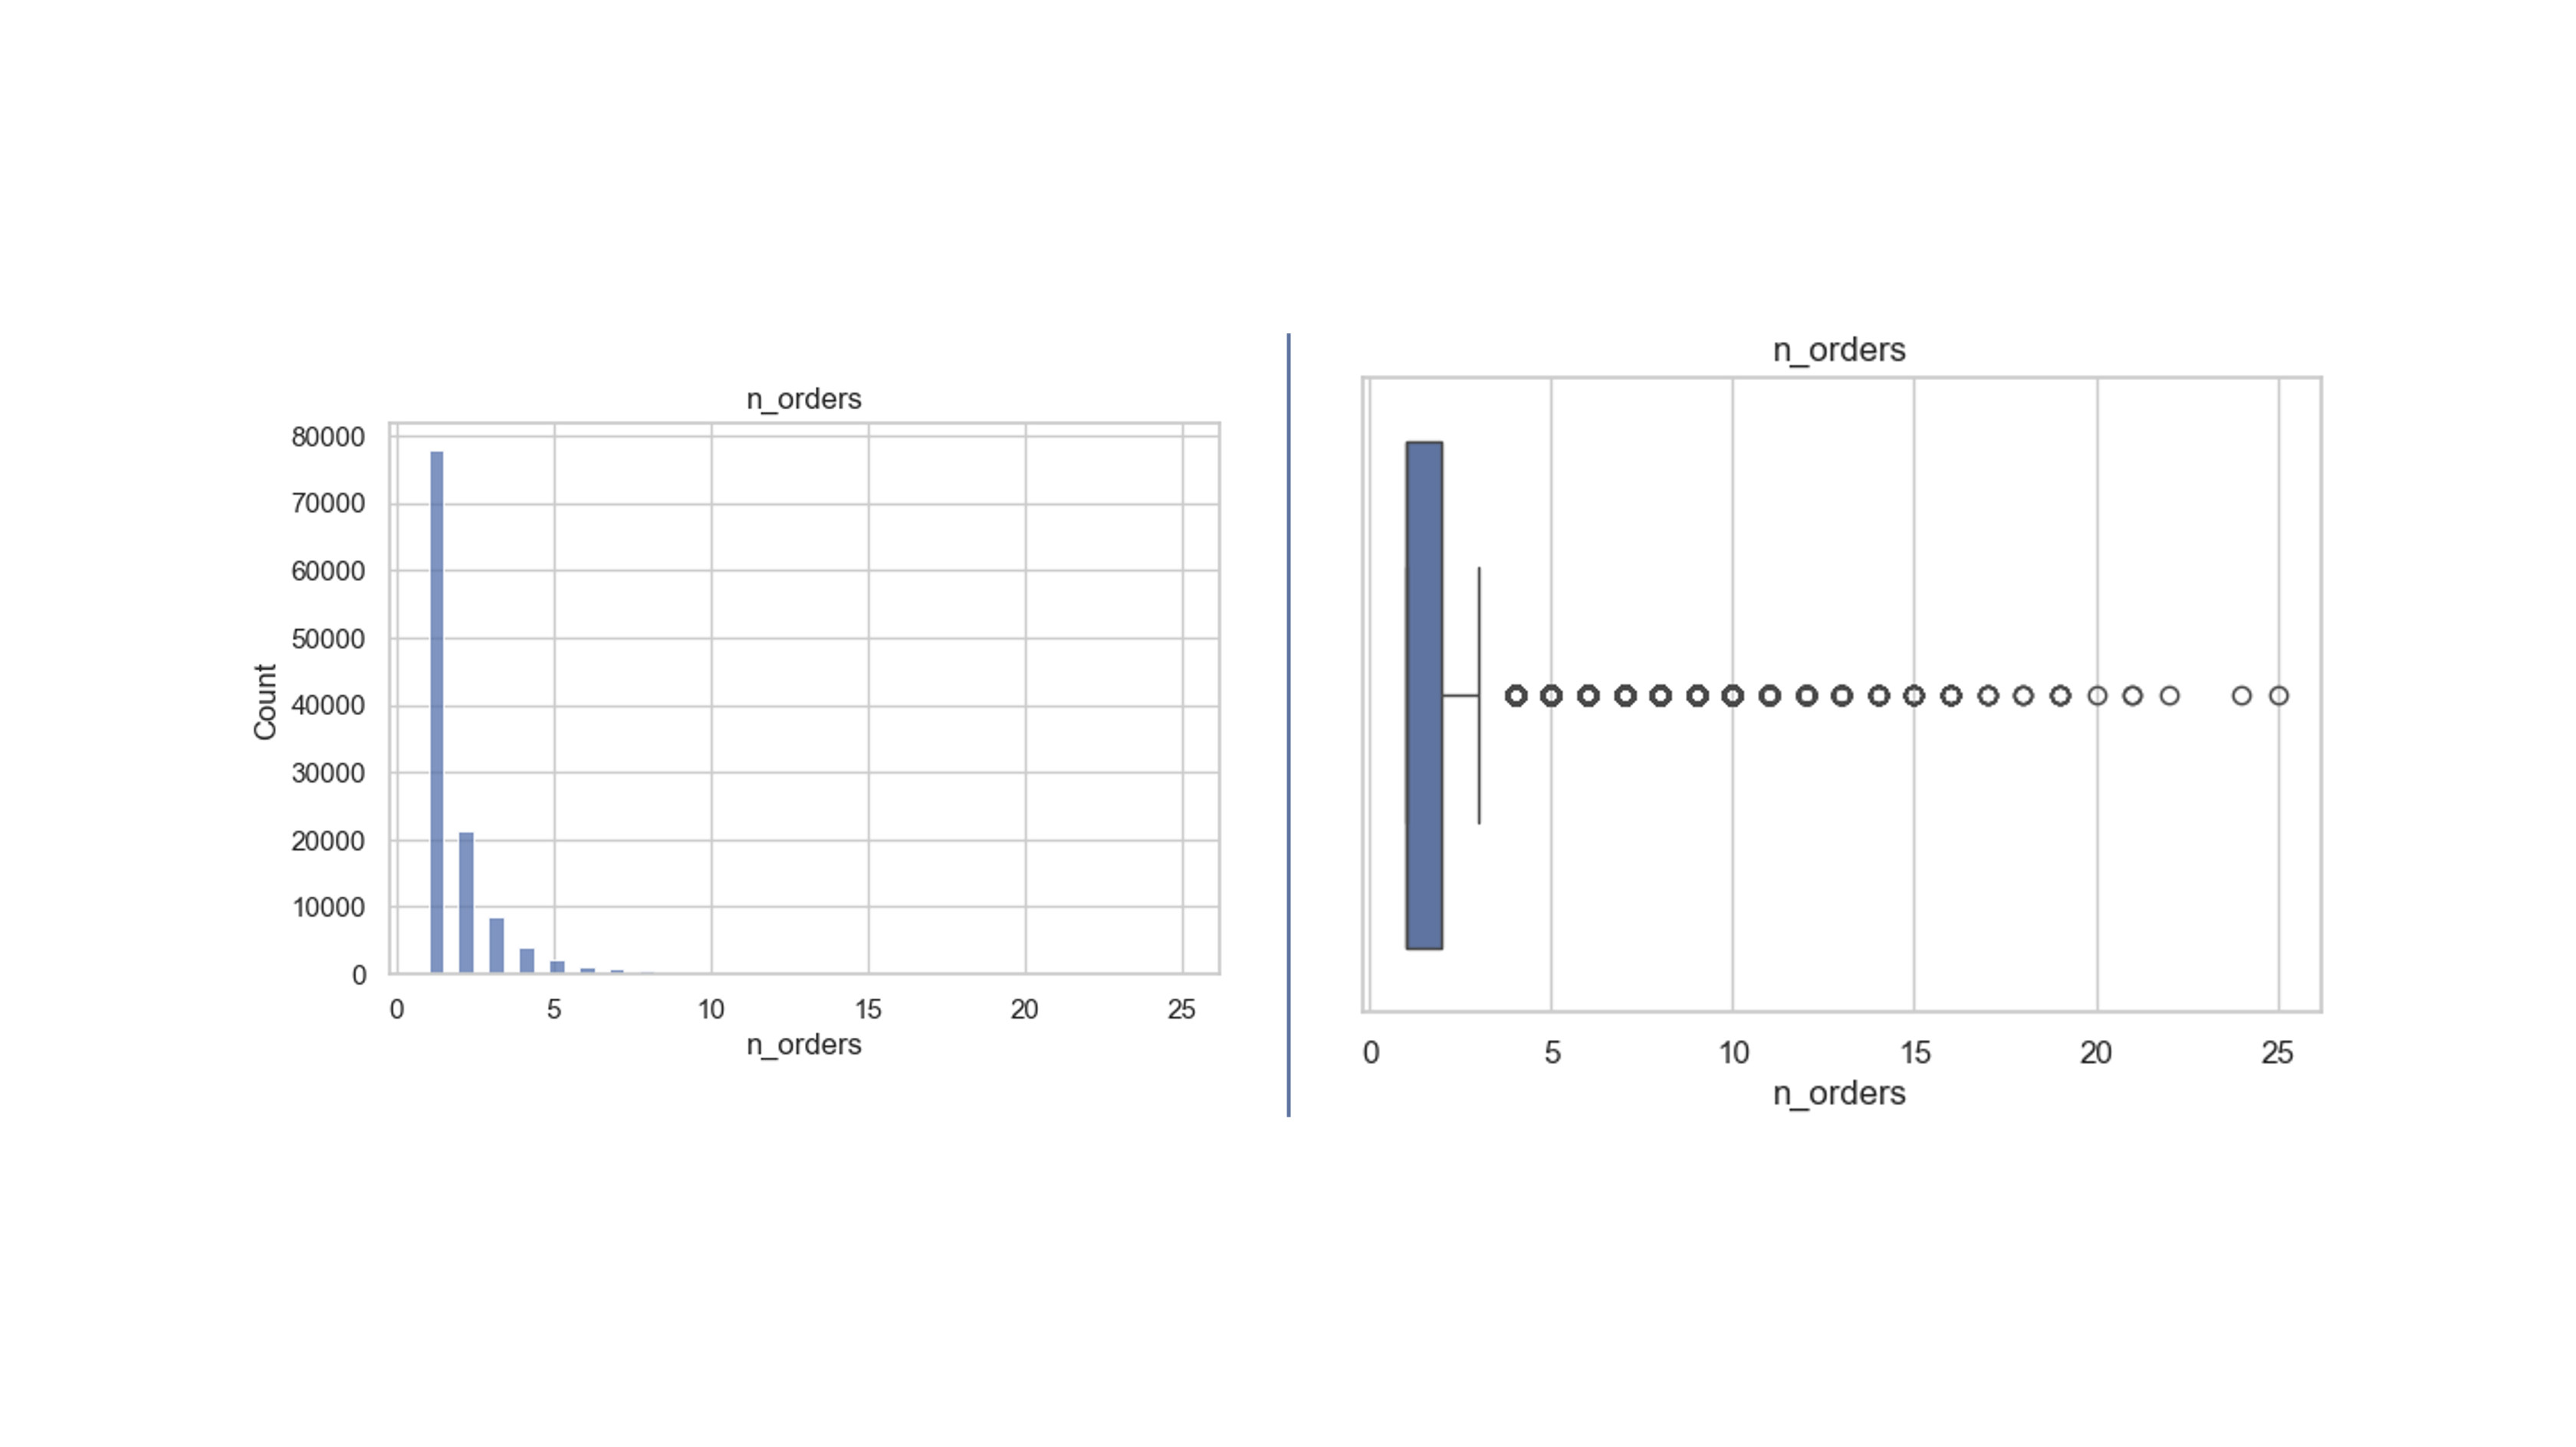
\includegraphics[width=1.2\textwidth]{figures/1 Distribution of purchases per customer.png}}
\caption{Distribution of purchases per customer.}
\end{figure}

Historical spending showed a right-skewed distribution with a mode near seventy-five euros and a median around one hundred euros. The interquartile range ran roughly from forty to two hundred euros, with a whisker extending to approximately three hundred euros and a long outlier tail reaching twelve hundred euros or more. The average order value was more symmetric, approximately bell-shaped and centred around sixty euros, with most customers falling between thirty and one hundred euros and outliers beginning above one hundred and forty euros.

\begin{figure}[H]
\centering
\makebox[\textwidth][c]{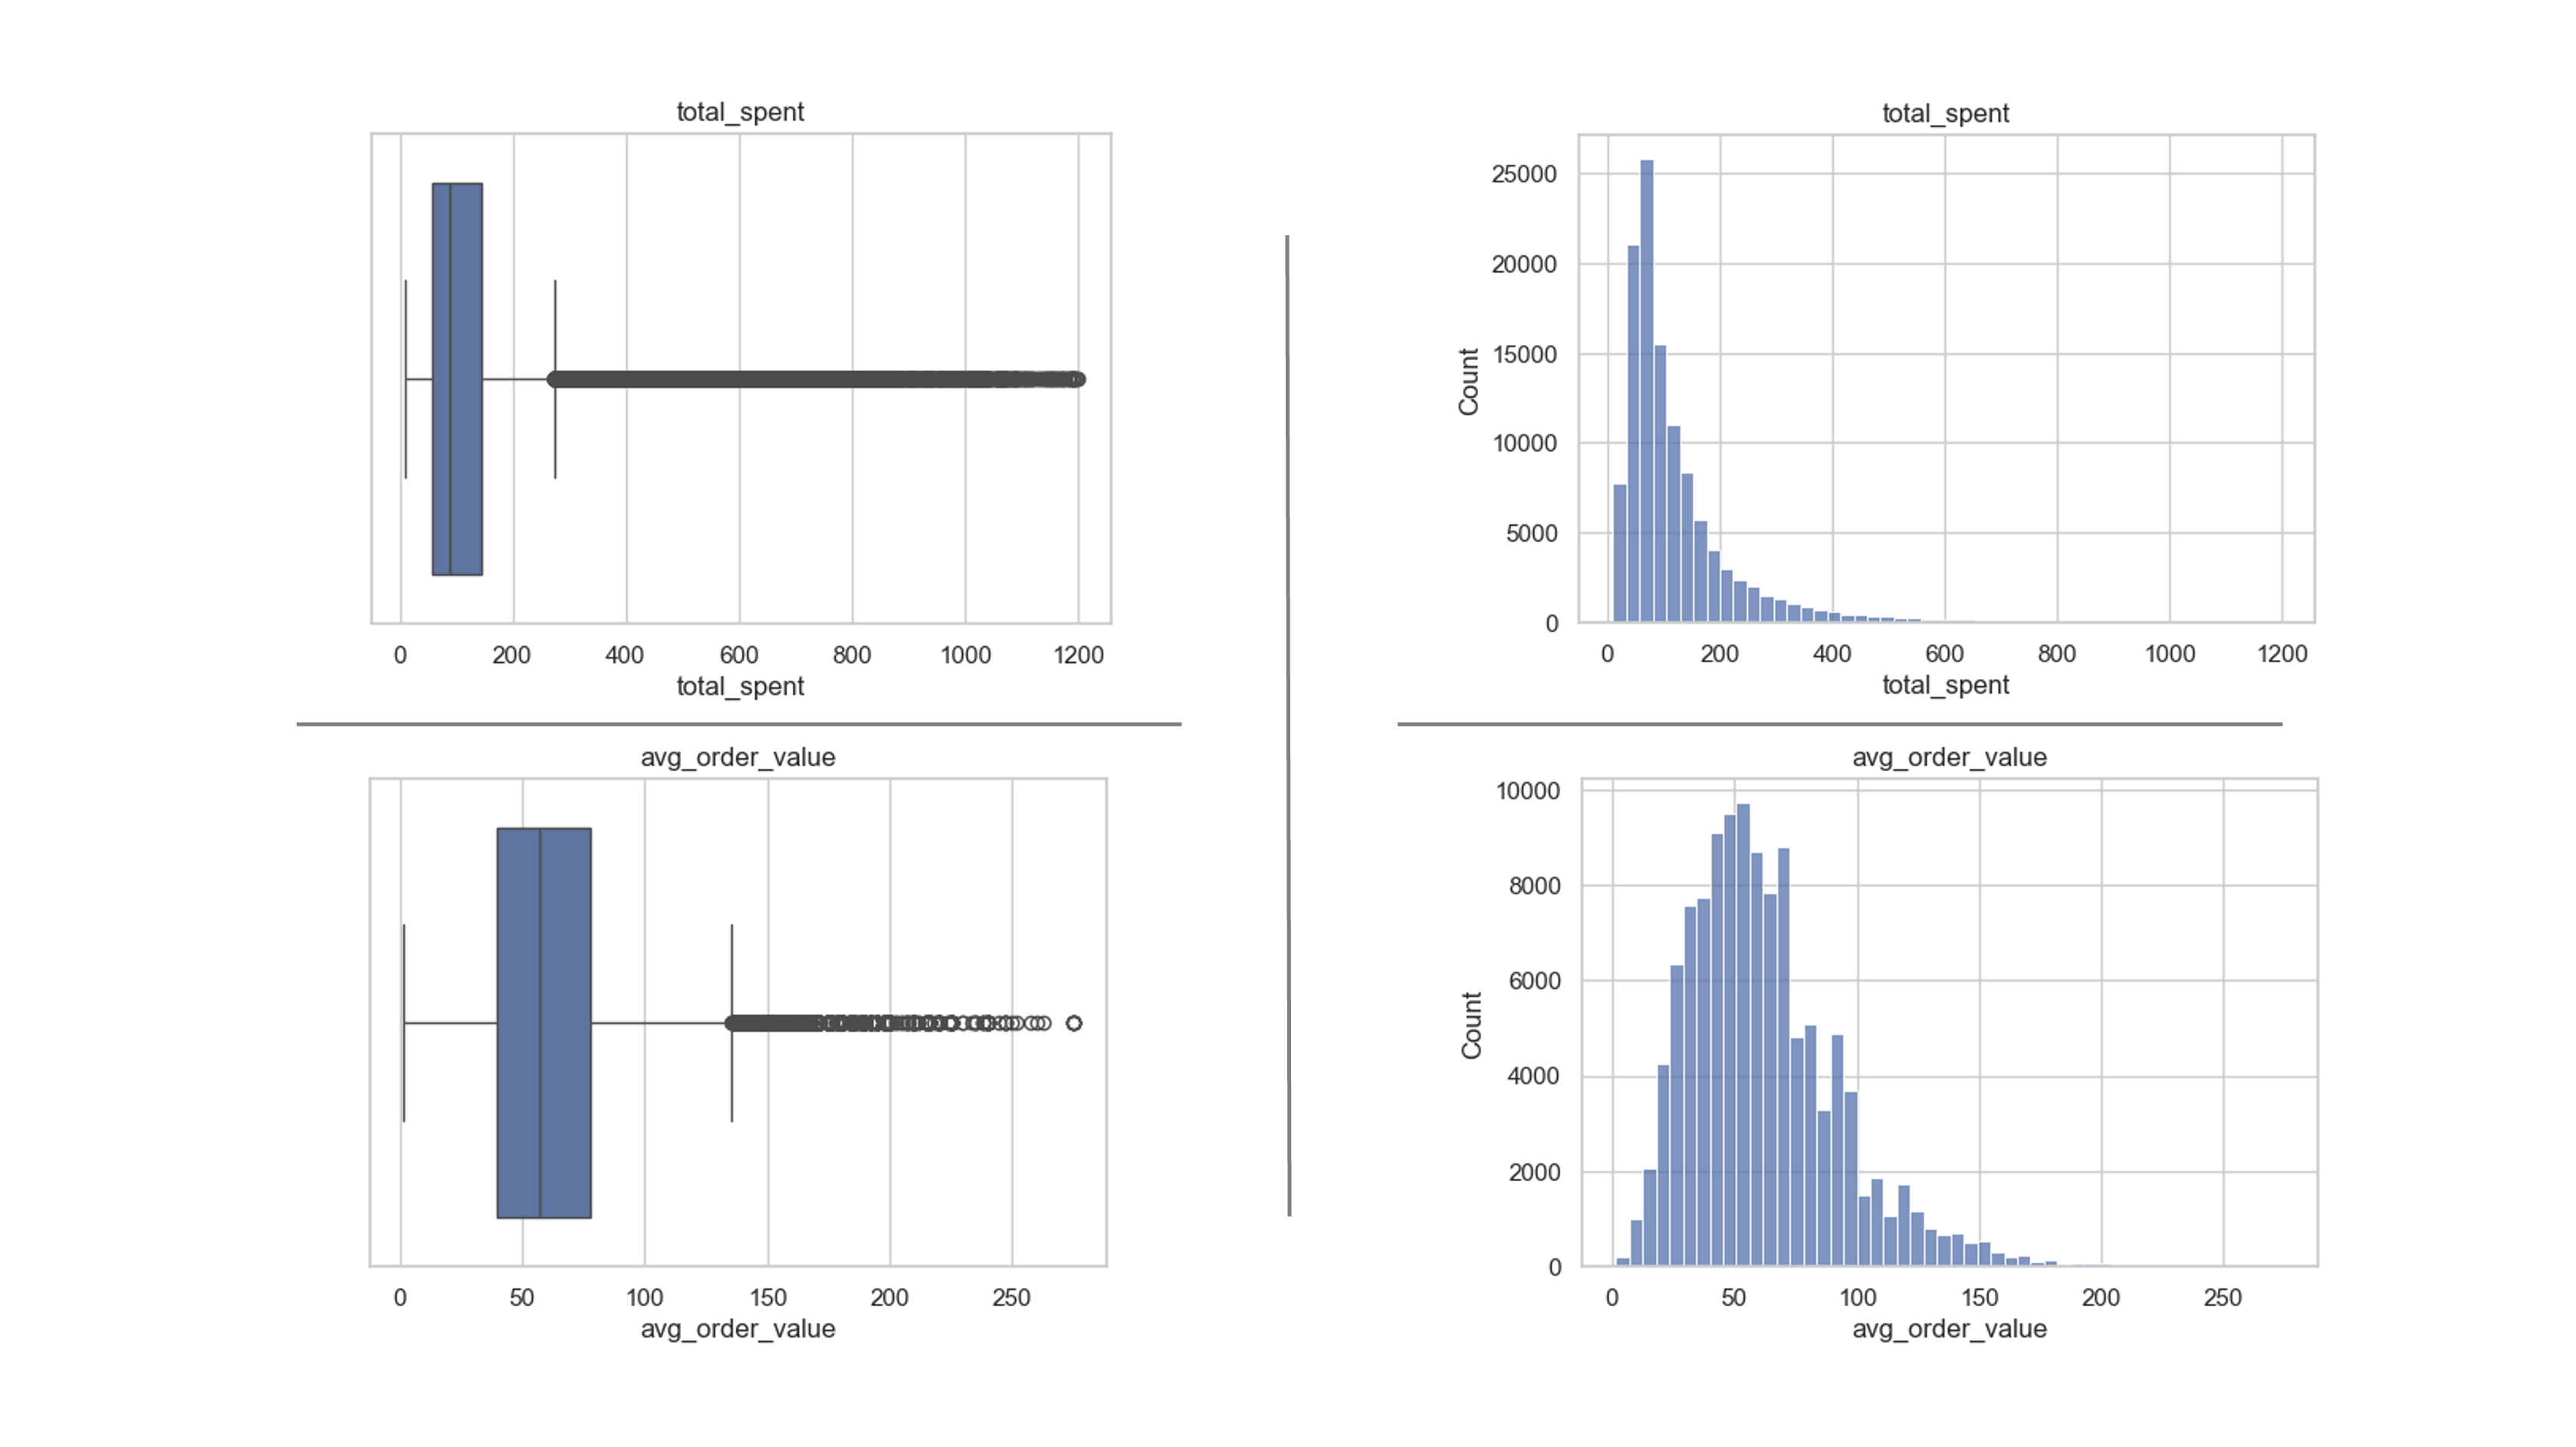
\includegraphics[width=1.2\textwidth]{figures/2 Historical spending.png}}
\caption{Historical spending distribution.}
\end{figure}

Recent activity, captured through revenue in the last ninety days, was overwhelmingly zero-concentrated. Approximately 97,000 out of 116,000 customers had no revenue at all in the final ninety days of the observation window. The small non-zero group showed a minor concentration around fifty to one hundred euros, tapering to rare outliers near seven hundred euros. This extreme sparsity makes revenue\_last\_90d a high-signal but difficult feature, functioning essentially as a binary indicator for most customers.



The purchase frequency distribution, measured as orders per day, showed a distinctive spike at approximately 0.033, corresponding to one order per thirty days. This spike arises from single-order customers whose customer lifetime is regularised by adding thirty days to the denominator. A spread of lower-frequency customers appeared between 0.003 and 0.025, with a small secondary bump near 0.06. Very few customers exceeded 0.08 orders per day.



The target variable, revenue\_2018\_2019, was massively zero-inflated. The first histogram bar (revenue approximately zero euros) contained approximately 74,000 of the 116,000 customers in the training set, representing around 64 percent. Among non-zero customers, the distribution remained heavily right-skewed, with most spending between twenty and two hundred euros and a gradually tapering tail reaching approximately twelve hundred euros. The log-transformed histogram revealed a bimodal structure: a dominant spike at zero (the churned customers) and a roughly uniform plateau between log-values of three and seven (corresponding to approximately twenty to eleven hundred euros in real revenue). This zero-inflation is the single biggest modelling challenge, as the model must simultaneously determine which customers will churn and predict how much active customers will spend.

\begin{figure}[H]
\centering
\makebox[\textwidth][c]{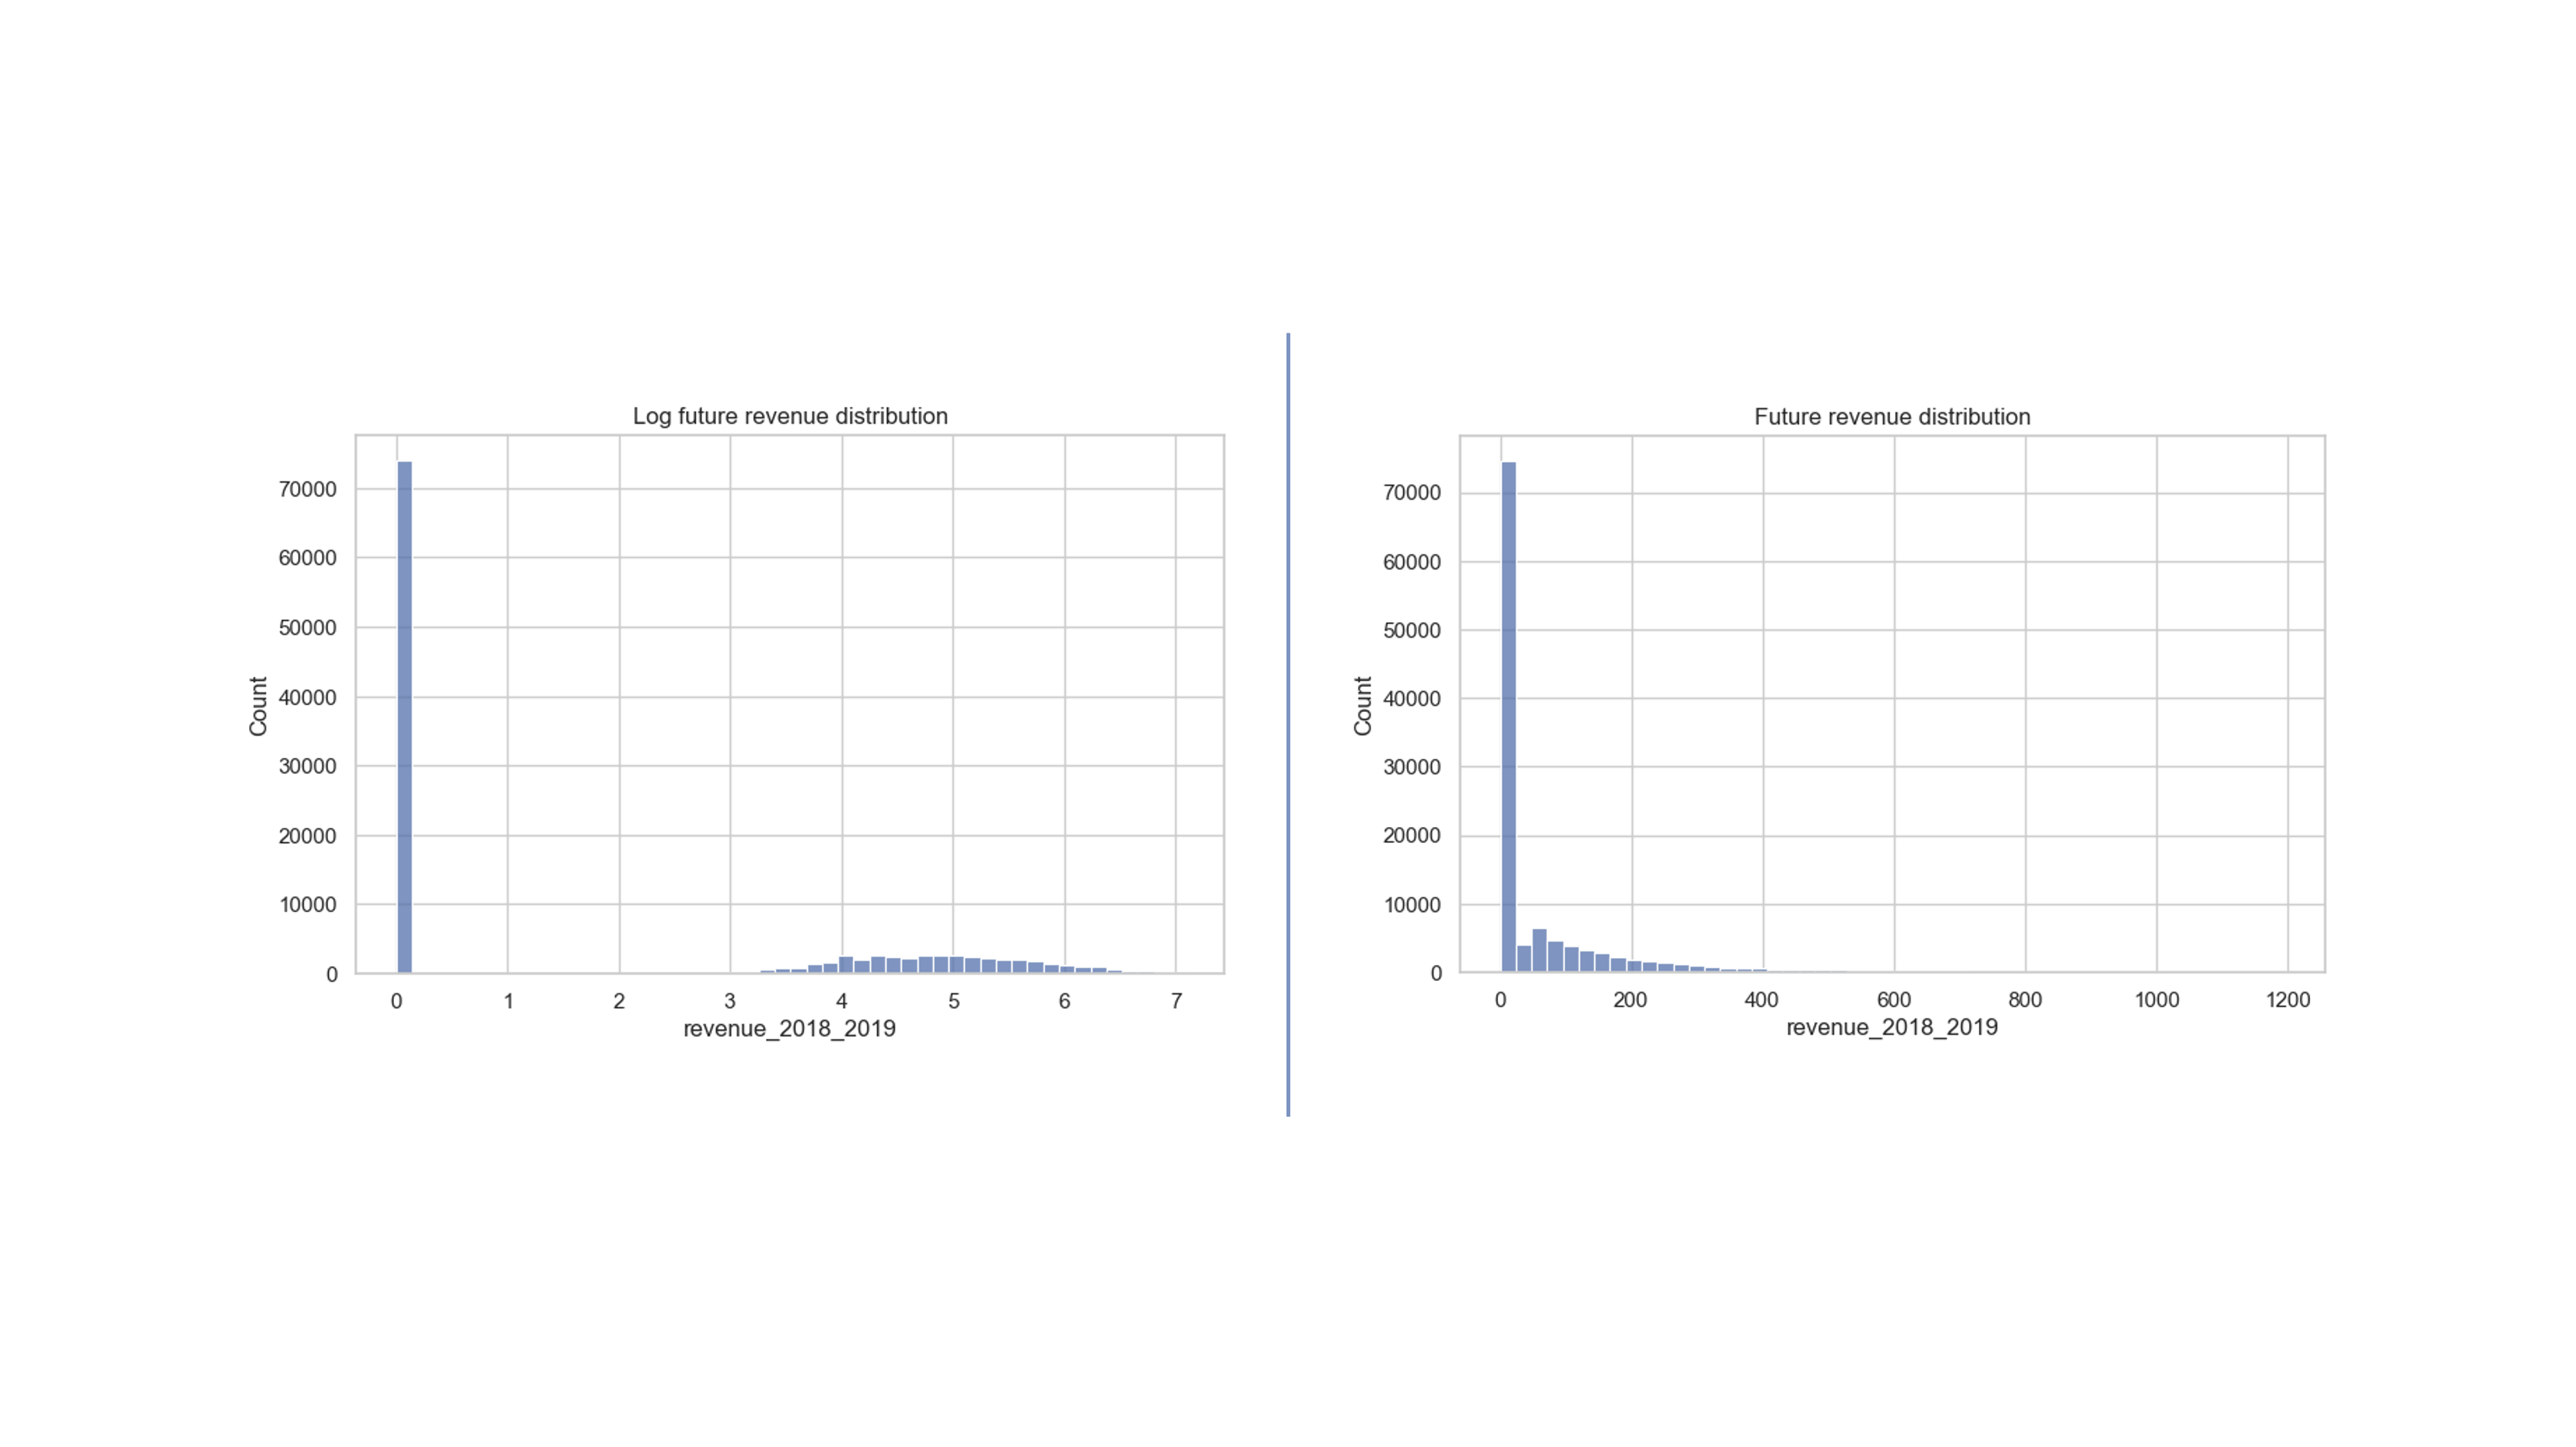
\includegraphics[width=1.2\textwidth]{figures/4 Target variable (revenue_2018_2019).png}}
\caption{Target variable distribution.}
\end{figure}

Recency was multi-modal and broadly distributed across the full 0 to 730 day observation window. The distribution had visible peaks near 0 to 50 days and 150 to 180 days, as well as a secondary cluster around 340 to 360 days. A dip around 400 to 430 days separated these clusters. This shows that the customer base is heterogeneous in terms of time since last purchase.
\begin{figure}[H]
\centering
\makebox[\textwidth][c]{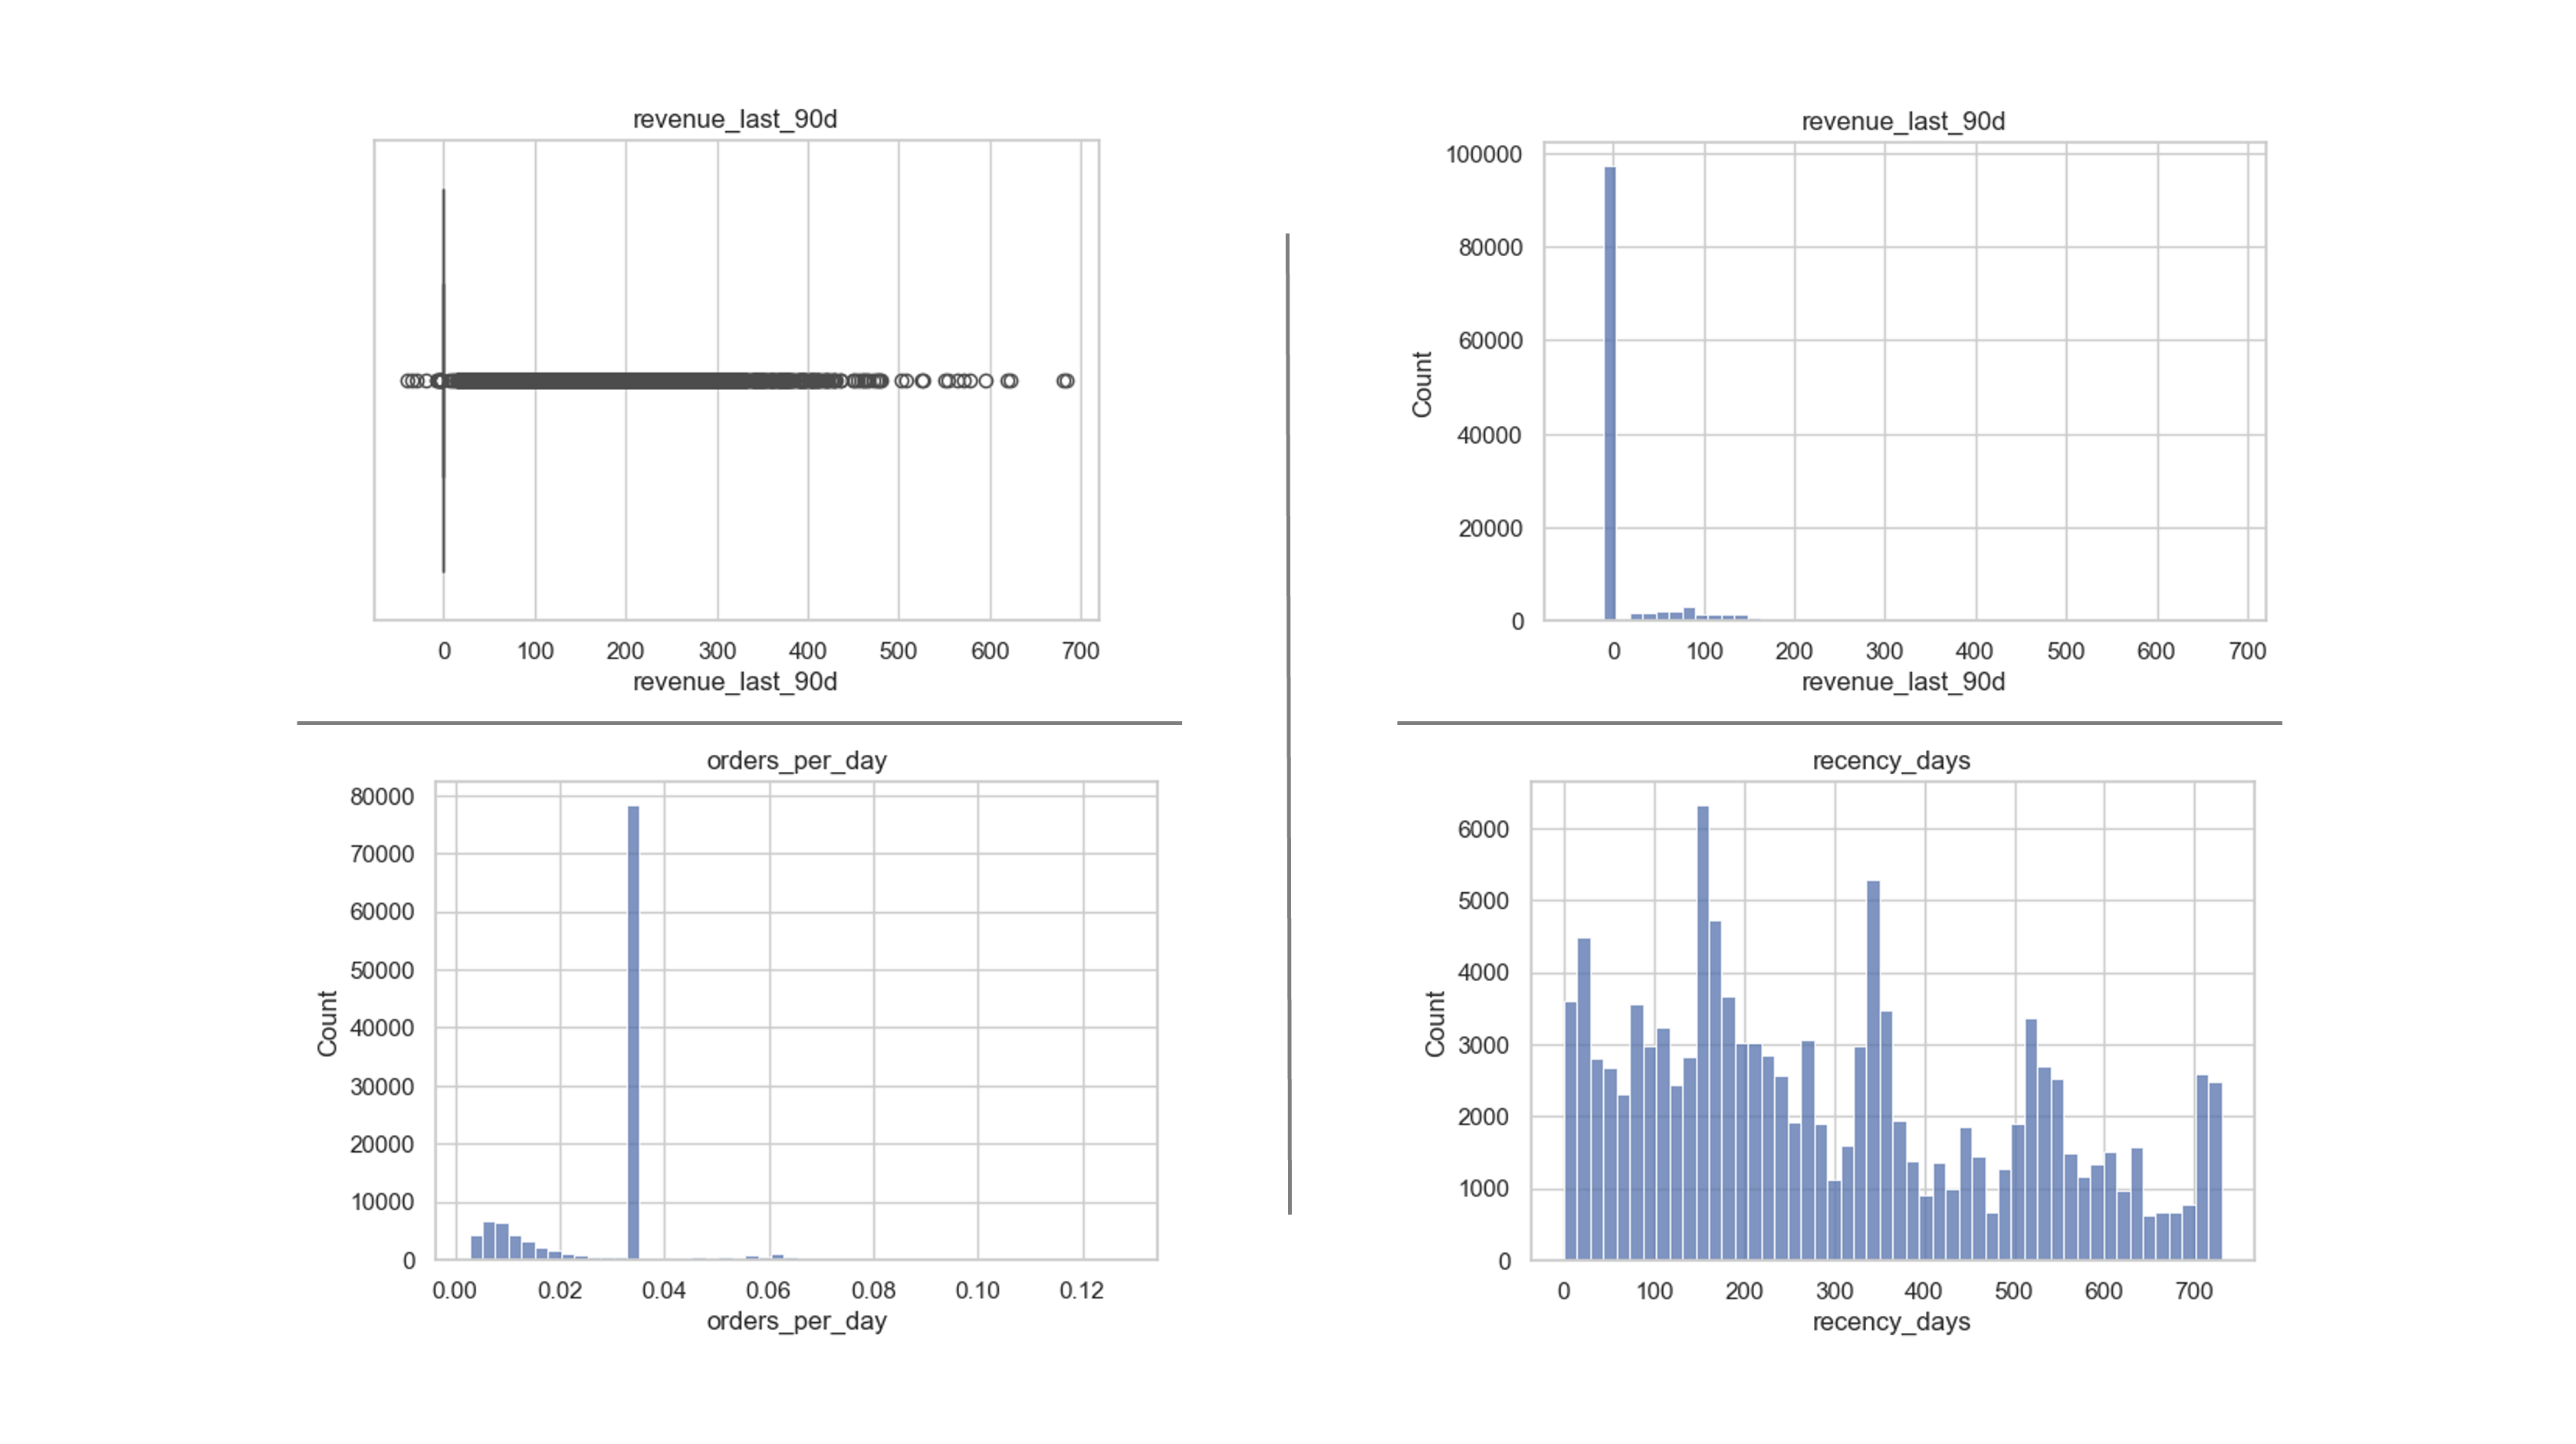
\includegraphics[width=1.2\textwidth]{figures/3 Recent activity purchase frequency recency distribution.png}}
\caption{Recent activity, purchase frequency, and recency distribution.}
\end{figure}

\subsection{Transaction patterns}
Recency showed a clear negative association with future revenue. The densest concentration of high-revenue customers, approximately 200 to 800 euros, appeared among customers with low recency values between 0 and 200 days. As recency increased beyond about 300 days, the point cloud thinned and revenue values trended downward. However, revenue equal to zero was densely present at all recency levels, meaning that even recently active customers could churn. A few high-revenue outliers appeared at recency values above 600 days, but these were rare exceptions.



Historical spending showed a positive but noisy association with future revenue. The densest portion of the scatterplot was concentrated in the zero to four hundred euro range for both historical spend and future revenue. High historical spenders showed a wide spread of outcomes, with some continuing to spend at high levels while others churned completely to zero. A thick band of zero future revenue ran along the entire x-axis, confirming that no amount of historical spending guarantees retention.



Purchase frequency also showed a complex relationship with future revenue. Single-order customers, clustered at approximately 0.033 orders per day, exhibited the full range of outcomes from zero to twelve hundred euros in future revenue. Higher-frequency customers (0.04 to 0.08 orders per day) showed denser clusters of non-zero future revenue, but with considerable variance. Customers with extremely high purchase frequency did not consistently translate to high future spending, and their data points were mostly concentrated near zero.



Return behaviour spanned the full range from zero to one hundred percent return rates. While there was no strong linear correlation between return rate and future CLV, the density of high-revenue customers was noticeably greater at lower return rates (zero to thirty percent) compared to very high return rates (eighty to one hundred percent), where most customers had near-zero future revenue. This suggests that extreme returners are less likely to convert, while moderate return rates do not meaningfully reduce future revenue.

\begin{figure}[H]
\centering
\makebox[\textwidth][c]{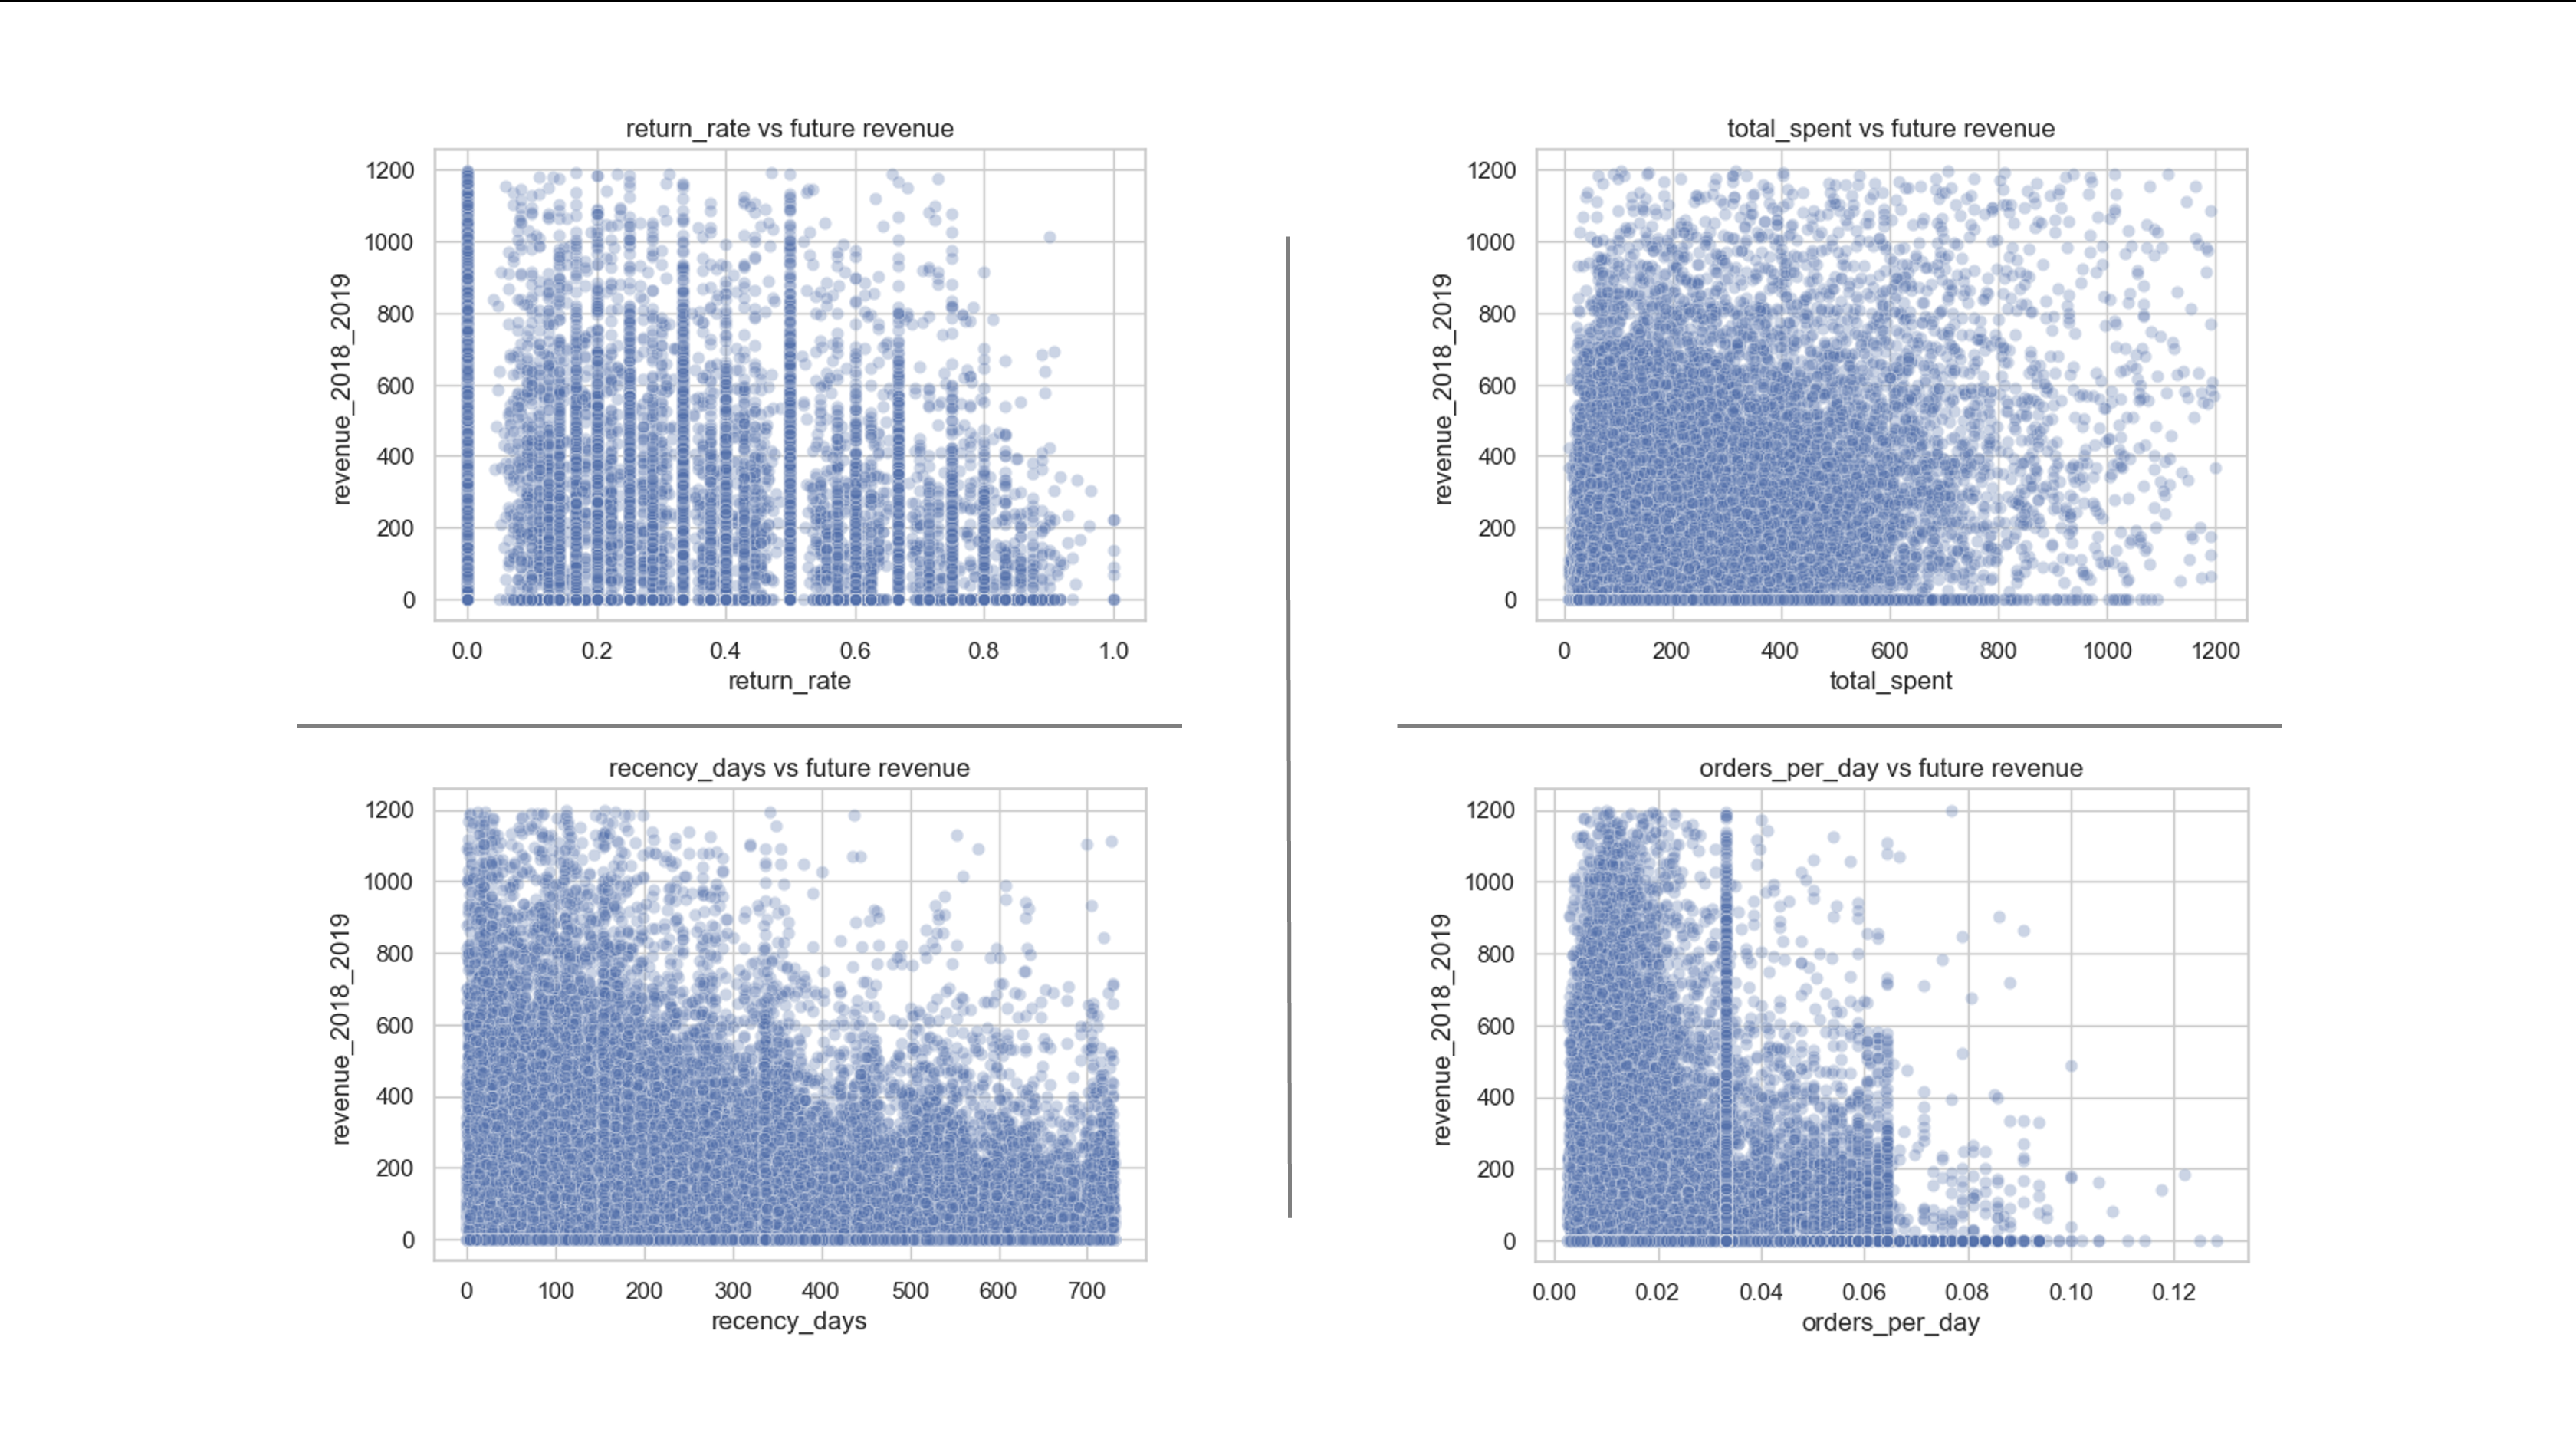
\includegraphics[width=1.2\textwidth]{figures/5 Transaction Patterns.png}}
\caption{Transaction patterns vs future revenue.}
\end{figure}

Seasonality and product preferences also showed useful structure. Product season codes such as W14 and W15 tied products to collection cycles, while purchase months were used to derive month\_std and unique\_months, capturing seasonal breadth. Brand concentration was high: a few brands, including Gabor, Geox, STONES and BONES, accounted for a disproportionate share of transactions, while hundreds of long-tail brands appeared rarely. The prod\_type\_1 feature encoded target demographic categories such as women, men, boys and girls, with women’s footwear dominating transaction volume.


A Pearson correlation analysis with the target variable confirmed the importance of volume and engagement features. The strongest positive correlators were total\_spent and n\_orders (both 0.44), n\_products (0.42), n\_colors (0.42), and n\_brands (0.41), all of which proxy overall customer engagement. The log\_total\_spent variable (0.37) and customer\_lifetime\_days (0.36) also ranked highly, confirming that both spending magnitude and relationship length are predictive. The favorite\_brand\_orders (0.32) and n\_categories (0.31) showed moderate positive association.

The strongest negative correlators were orders\_per\_day\_raw (-0.34), total\_discount (-0.27), favorite\_brand\_share (-0.27), and orders\_per\_day (-0.26), suggesting that high purchase frequency per day and deeper discounting are associated with lower future revenue. The recency\_days variable had a correlation of -0.21, confirming the visual pattern from the scatterplot. Notably, avg\_order\_value (-0.05) and last\_order\_value (-0.02) were near zero, indicating that spending per order is essentially uncorrelated with future CLV. Features such as spending\_trend and outlet\_rate also showed near-zero linear correlations, though they may still contribute through non-linear interactions in tree-based models.

\begin{figure}[H]
\centering
\makebox[\textwidth][c]{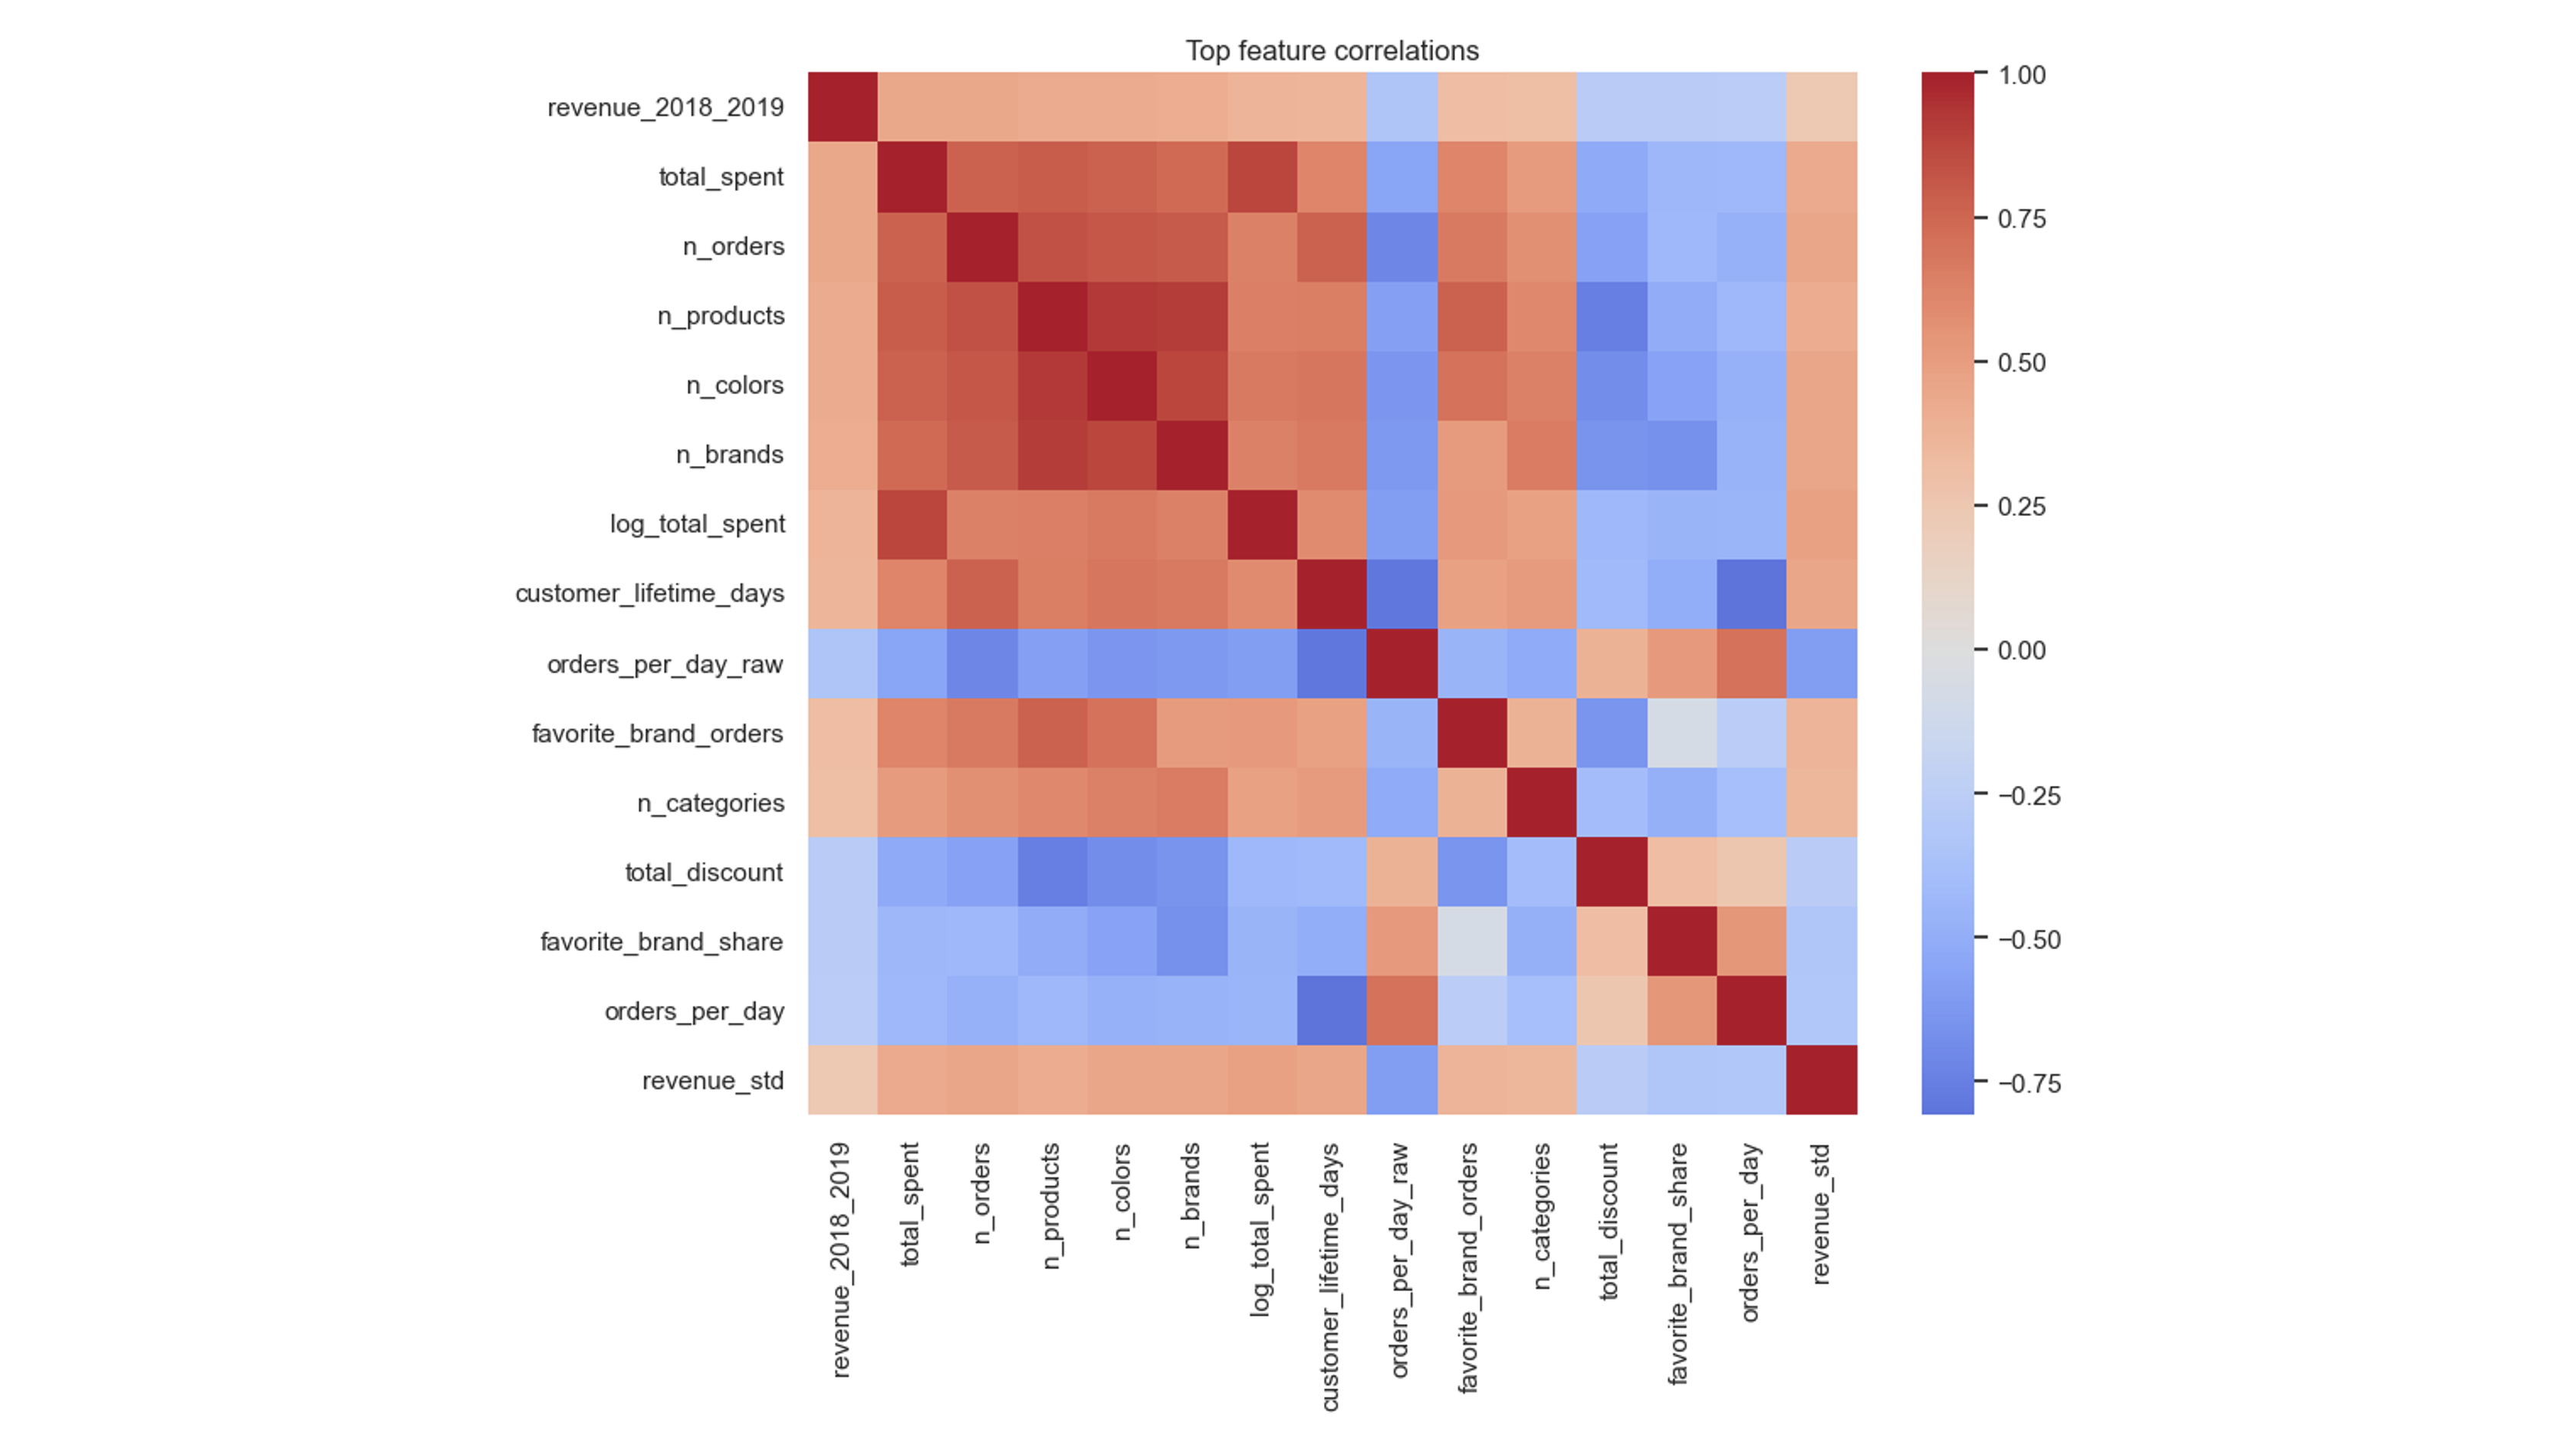
\includegraphics[width=1.2\textwidth]{figures/6 Correlation with target.png}}
\caption{Pearson correlation with target variable.}
\end{figure}

\subsection{Key observations}
The exploratory analysis produced several important modelling implications. First, zero-inflation dominates the prediction problem, with approximately 64% of customers having zero future revenue. This means the model must address a mixed classification-regression problem: it must identify likely churners while still estimating revenue for active customers. This motivated hurdle-model experiments and zero-rate post-processing.
Second, volume features were the strongest predictors. total\_spent, n\_orders and n\_products had the highest linear correlations with the target and all captured customer engagement. These variables are mutually related, creating multicollinearity, but tree-based models can handle such overlap effectively. Third, recency was the strongest negative signal, both visually and numerically, and motivated recency-based post-processing rules that reduced or zeroed predictions for highly inactive customers.
Fourth, per-order value was much less informative than total activity. Average order value was nearly uncorrelated with future customer lifetime value, so the frequency and breadth of engagement mattered more than isolated transaction size. Fifth, discount-heavy customers tended to churn, as total\_discount and orders\_per\_day\_raw were negatively correlated with future revenue. Sixth, the target and several features were strongly right-skewed, supporting the use of log-transformed variables and MAE-based objectives.
Finally, high-cardinality and multi-label fields required careful treatment. Rare brands and rare tokens were grouped to reduce dimensionality and noise. Recent activity variables such as revenue\_last\_90d and orders\_last\_90d were disproportionately informative despite being zero for most customers. Outliers were preserved because the chosen tree-based models can handle them and because high-value customers are a meaningful part of the customer lifetime value distribution.

\section{Data preprocessing}
Before constructing the feature matrix, the dataset was partitioned based on the availability of the target variable revenue\_2018\_2019. Customers with known purchase outcomes constituted the training set, while the unlabelled customers formed the test set for which final predictions were generated. This separation ensured that the model was trained strictly on historical ground truth before being applied to the future prediction window.

\subsection{Cleaning}
Missing values were addressed using domain-specific imputations. The most substantial case involved 280,282 missing return identifiers, which were interpreted as indicating no return and filled accordingly. Additionally, 132,201 missing heel-type records were handled, and numeric size gaps were filled via median imputation to ensure a complete feature matrix for the 274,311 training rows. The 1,063 duplicate rows (approximately 0.31 percent of the dataset) were removed after applying a temporary conversion of multi-label list columns to tuples to enable hashing.

To prevent extreme high-value transactions from disproportionately influencing the model, the MAE (L1) objective was used, which is naturally robust to outliers. Additionally, high-cardinality grouping was applied, merging brands and attributes with low support below a defined minimum count threshold (< 1000 for brands, <300 for any other category with a high cardinality) into an 'Other' category.

Noise was present in several forms. The prod\_size column contained mixed types, including both numeric shoe sizes and the text value 'XS', and non-numeric entries were coerced to missing. Categorical fields required standardisation through lowercasing, whitespace trimming, and separator normalisation. High-cardinality fields such as prod\_brand, which contained hundreds of unique values, introduced noise, and rare brands with fewer than 1,000 occurrences were grouped into an 'other\_brand' category to reduce dimensionality without discarding useful signal. A similar grouping strategy was applied to rare tokens in multi-label fields, with tokens appearing fewer than 300 times collapsed into an 'other' category.

A text standardisation pipeline was applied to transaction attributes, involving lowercasing, removal of punctuation, and alphabetical sorting of multi-label string tokens. This ensured that entries such as 'Blue, Red' and 'red, blue' were treated as identical. Binary status indicators, such as return flags and outlet purchase indicators, were coerced into a uniform integer format (1/0) to ensure compatibility with the modelling framework and to simplify downstream calculations.

\subsection{Feature engineering}
Feature engineering was a central and critical component of this project. The raw transaction log was transformed into a unified customer profile by grouping records by cust\_id, converting 274,311 individual purchase events into a behavioural matrix in which each row represents a unique customer's entire purchasing history.

A range of features was constructed to capture different aspects of customer behaviour. Total revenue was calculated as the lifetime gross spend per customer, and showed a Pearson correlation of 0.44 with the target revenue. The total number of purchases was computed as the count of orders placed, capturing the breadth of the customer's relationship with the retailer. Average order value (AOV) was derived by dividing total revenue by the number of orders, distinguishing high-ticket shoppers from those who make frequent lower-value purchases.

Recency, defined as the number of days since the customer's most recent transaction, was used both as a predictive feature and as a basis for post-processing rules applied to customers identified as likely churned. Frequency was measured as the rate of purchase over the customer's lifetime to identify regular repeat buyers. Product-based features captured the customer's favourite brand, determined by identifying the most frequently purchased brand per customer and applying frequency encoding to capture market-share signals and brand loyalty patterns.

Temporal features included a seasonal pulse variable, derived as the standard deviation of purchase months. This distinguishes customers who buy only during specific sales periods or holidays from those who shop year-round. Return behaviour was captured as the ratio of returned items to total items purchased, serving as a profitability filter since high return rates often reduce net revenue relative to gross spend. Short-term behaviour features tracked revenue and order counts in the last ninety days, capturing momentum for customers in an active buying phase. Finally, customer activity velocity features measured the average time between orders and the rate of engagement over the customer's lifetime to estimate the timing of the next likely purchase.

\subsection{Encoding and transformation}
For the tree-based models used in this project, categorical variables such as favourite brand were converted into category codes (label encoding). This allowed the models to split efficiently on brand identity without the memory overhead and sparsity issues associated with one-hot encoding.

Formal feature scaling was not applied because tree-based models are invariant to the scale of input features, preserving the interpretability of the original units (days, euros) during the analysis phase. Log-transformations were applied to highly skewed financial variables, including total\_spent (skewness 3.19) and AOV (skewness 1.08), using a log(1+x) transformation. This compressed the long tail of high spenders and prevented extreme outliers from dominating the loss function.

Frequency encoding was implemented for high-cardinality categorical variables. By mapping brands to their overall frequency in the dataset, the model received a continuous popularity signal, helping it differentiate between customers who favour market-leading brands and those who purchase from niche brands with different spending velocity patterns.

\section{Modelling}
\subsection{General modelling approach}
The modelling task was formulated as a supervised regression problem in which the goal was to predict future customer revenue from historical transaction behaviour. Since the raw data was transaction-level, the first step was aggregating it to the customer level, producing a feature matrix with one row per customer suitable for supervised learning.

Feature engineering focused on capturing customer behaviour across several groups: purchase activity features (number of orders, number of products), financial features (total spending, average order value), temporal features (recency, customer lifetime), return and discount behaviour, product diversity and loyalty measures, and more advanced behavioural features such as spending stability and seasonal shopping patterns.

Because the target variable was heavily right-skewed and contained many zero-revenue customers, MAE was used as the main optimisation metric throughout the project. MAE is less dominated by a small number of extreme high-revenue customers compared to squared-error losses. Several model families were explored, but the final pipeline focused on gradient boosting tree models, which are well suited for heterogeneous tabular business data and can naturally model non-linear interactions between behavioural variables. The main models used were LightGBM, CatBoost, and XGBoost. Cross-validation was used throughout to estimate generalisation performance, and early stopping was applied to prevent overfitting.

\subsection{Lightgbm models}
LightGBM was the strongest model family throughout experimentation and consistently achieved the best validation scores. The initial LightGBM models already performed competitively, but performance improved significantly after incorporating more advanced behavioural features and stronger regularisation. The final LightGBM setup relied on MAE/L1 optimisation, Gradient-based One-Side Sampling (GOSS), low learning rates, conservative tree growth, strong regularisation, and extensive early stopping.

Optimising directly for MAE aligned the training objective with the competition metric and produced more stable predictions on the highly skewed target distribution. GOSS was used because it focuses more strongly on difficult observations while sampling easier cases more aggressively, allowing the model to remain efficient while still learning from customers with unusual spending behaviour. Strong regularisation and large minimum leaf sizes made the model more conservative and reduced overfitting on noisy customer patterns. Several post-processing strategies were tested on top of the LightGBM predictions. Experiments showed that moderate behavioural adjustments improved performance slightly, while overly aggressive filtering strongly degraded results. The strongest LightGBM models achieved an MAE of approximately 62.39 and a Spearman correlation of approximately 0.412.

\subsection{Catboost models}
CatBoost was explored as a second major boosting model because of its design for tabular data with categorical variables. Its ability to process categorical information without extensive manual encoding was particularly useful given the many behavioural and product-related categorical variables in the dataset. The CatBoost setup used MAE optimisation, low learning rates, regularisation, subsampling, early stopping, and cross-validation. Different variants were explored, including experiments with Tweedie loss functions, though the standard MAE-based configuration remained more stable. CatBoost consistently produced competitive results, with an MAE of approximately 62.44 to 62.53 and a Spearman correlation of approximately 0.41. Although CatBoost was not the final best standalone model, it remained valuable for the ensemble stage due to the diversity of its predictions.

\subsection{Xgboost models}
XGBoost was used as the third major boosting model. The XGBoost setup focused on MAE optimisation, histogram-based tree construction, feature and row subsampling, regularisation, and early stopping. Compared to the other models, XGBoost relied more heavily on numerical behavioural features and a simpler preprocessing pipeline. It achieved an MAE of approximately 62.51 and a Spearman correlation of approximately 0.40. Despite not being the strongest standalone model, XGBoost captured different error patterns than CatBoost and LightGBM, which improved ensemble robustness.

\subsection{Hurdle and tweedie experiments}
Because the target distribution contained many zero-revenue customers and a strong positive tail, several alternative modelling approaches were explored. A hurdle-style model separated the problem into two stages: first predicting whether a customer would spend at all, and then predicting how much the customer would spend conditional on spending. Rather than applying a hard classification threshold, the final hurdle prediction combined both stages by multiplying the estimated spending probability with the predicted spending amount. Tweedie regression was also explored because the Tweedie distribution is theoretically well suited for zero-inflated positive targets such as customer revenue.

Although both approaches were theoretically appealing, experiments showed that they did not outperform the strongest direct MAE-based LightGBM models. In practice, directly optimising MAE with carefully engineered behavioural features proved more effective than explicitly modelling the zero-inflated structure of the target.

\subsection{Ensemble modelling}
After training the individual boosting models, several ensemble approaches were explored. The final ensemble combined predictions from LightGBM, CatBoost, and XGBoost. Different ensemble strategies were tested, including weighted averaging, median blending, and combinations thereof. Ensemble weights were optimised directly on validation predictions with the goal of minimising MAE. Median blending was additionally explored to reduce the influence of extreme prediction errors from individual models.

The ensemble models produced robust and stable predictions with an MAE of approximately 62.40 and a Spearman correlation of approximately 0.411. However, the ensemble only marginally improved robustness and did not outperform the strongest standalone LightGBM model.

\subsection{Post-processing}
A significant portion of experimentation focused on post-processing the raw model outputs. Because the dataset was heavily zero-inflated, the raw boosting models frequently produced many small positive revenue predictions for customers who were likely inactive. Several behavioural adjustment techniques were therefore explored to better calibrate churn behaviour and reduce low-confidence positive predictions.

Recency-based penalties were applied in two forms. In the more aggressive configuration, customers inactive for more than 500 days were forced directly to zero, while customers inactive for 400 to 500 days had their predictions multiplied by 0.2. In a smoother configuration, customers inactive for more than 450 days received a 50 percent prediction penalty, and those inactive for more than 600 days received an additional 80 percent penalty. Customers with extremely high return rates above 85 percent received an additional 50 percent prediction penalty. Very small predicted revenues below five euros were forced to zero to reduce low-confidence noise predictions and better match the sparsity structure of the target distribution.

Several experiments also explicitly forced a proportion of the lowest predictions to zero, with the optimal zero rate tuned around the observed training zero rate using cross-validation. Predictions were additionally calibrated using optimised scaling factors and upper clipping thresholds, with some experiments clipping at the 99th percentile of the training revenue distribution to reduce extreme outlier predictions. Distributional calibration techniques including quantile mapping and prediction snapping were also explored.

The experiments showed that moderate behavioural filtering slightly improved MAE, while overly aggressive zero forcing removed useful positive-revenue signal and worsened performance. Conservative recency-based adjustments consistently improved MAE slightly, while forcing extremely high zero rates usually degraded performance considerably. This indicates that balancing churn detection with preserving useful positive predictions was more important than aggressively pushing predictions to zero.

\subsection{Best-performing model}
The strongest overall model was an advanced LightGBM model combined with conservative behavioural post-processing. The final model combined advanced customer-level behavioural features, MAE/L1 optimisation, GOSS boosting, strong regularisation, cross-validation, and moderate recency-based post-processing. The best experiments achieved an MAE of approximately 62.39, a Spearman correlation of approximately 0.412, and a zero prediction rate of around 72 to 73 percent. The strongest model was therefore not the hurdle model, the Tweedie model, or the final ensemble, but a relatively robust and conservative LightGBM setup with carefully engineered behavioural features.

\section{Model comparison and prediction diagnostics}
\subsection{Overall model performance}
All gradient boosting models achieved relatively similar predictive performance. The advanced LightGBM model obtained the lowest MAE, while the Tweedie model achieved the worst MAE, likely due to overly aggressive zero predictions. Differences between the CatBoost, LightGBM, and XGBoost baseline models were relatively small, suggesting that feature engineering contributed more to performance than model selection alone.

\begin{figure}[H]
\centering
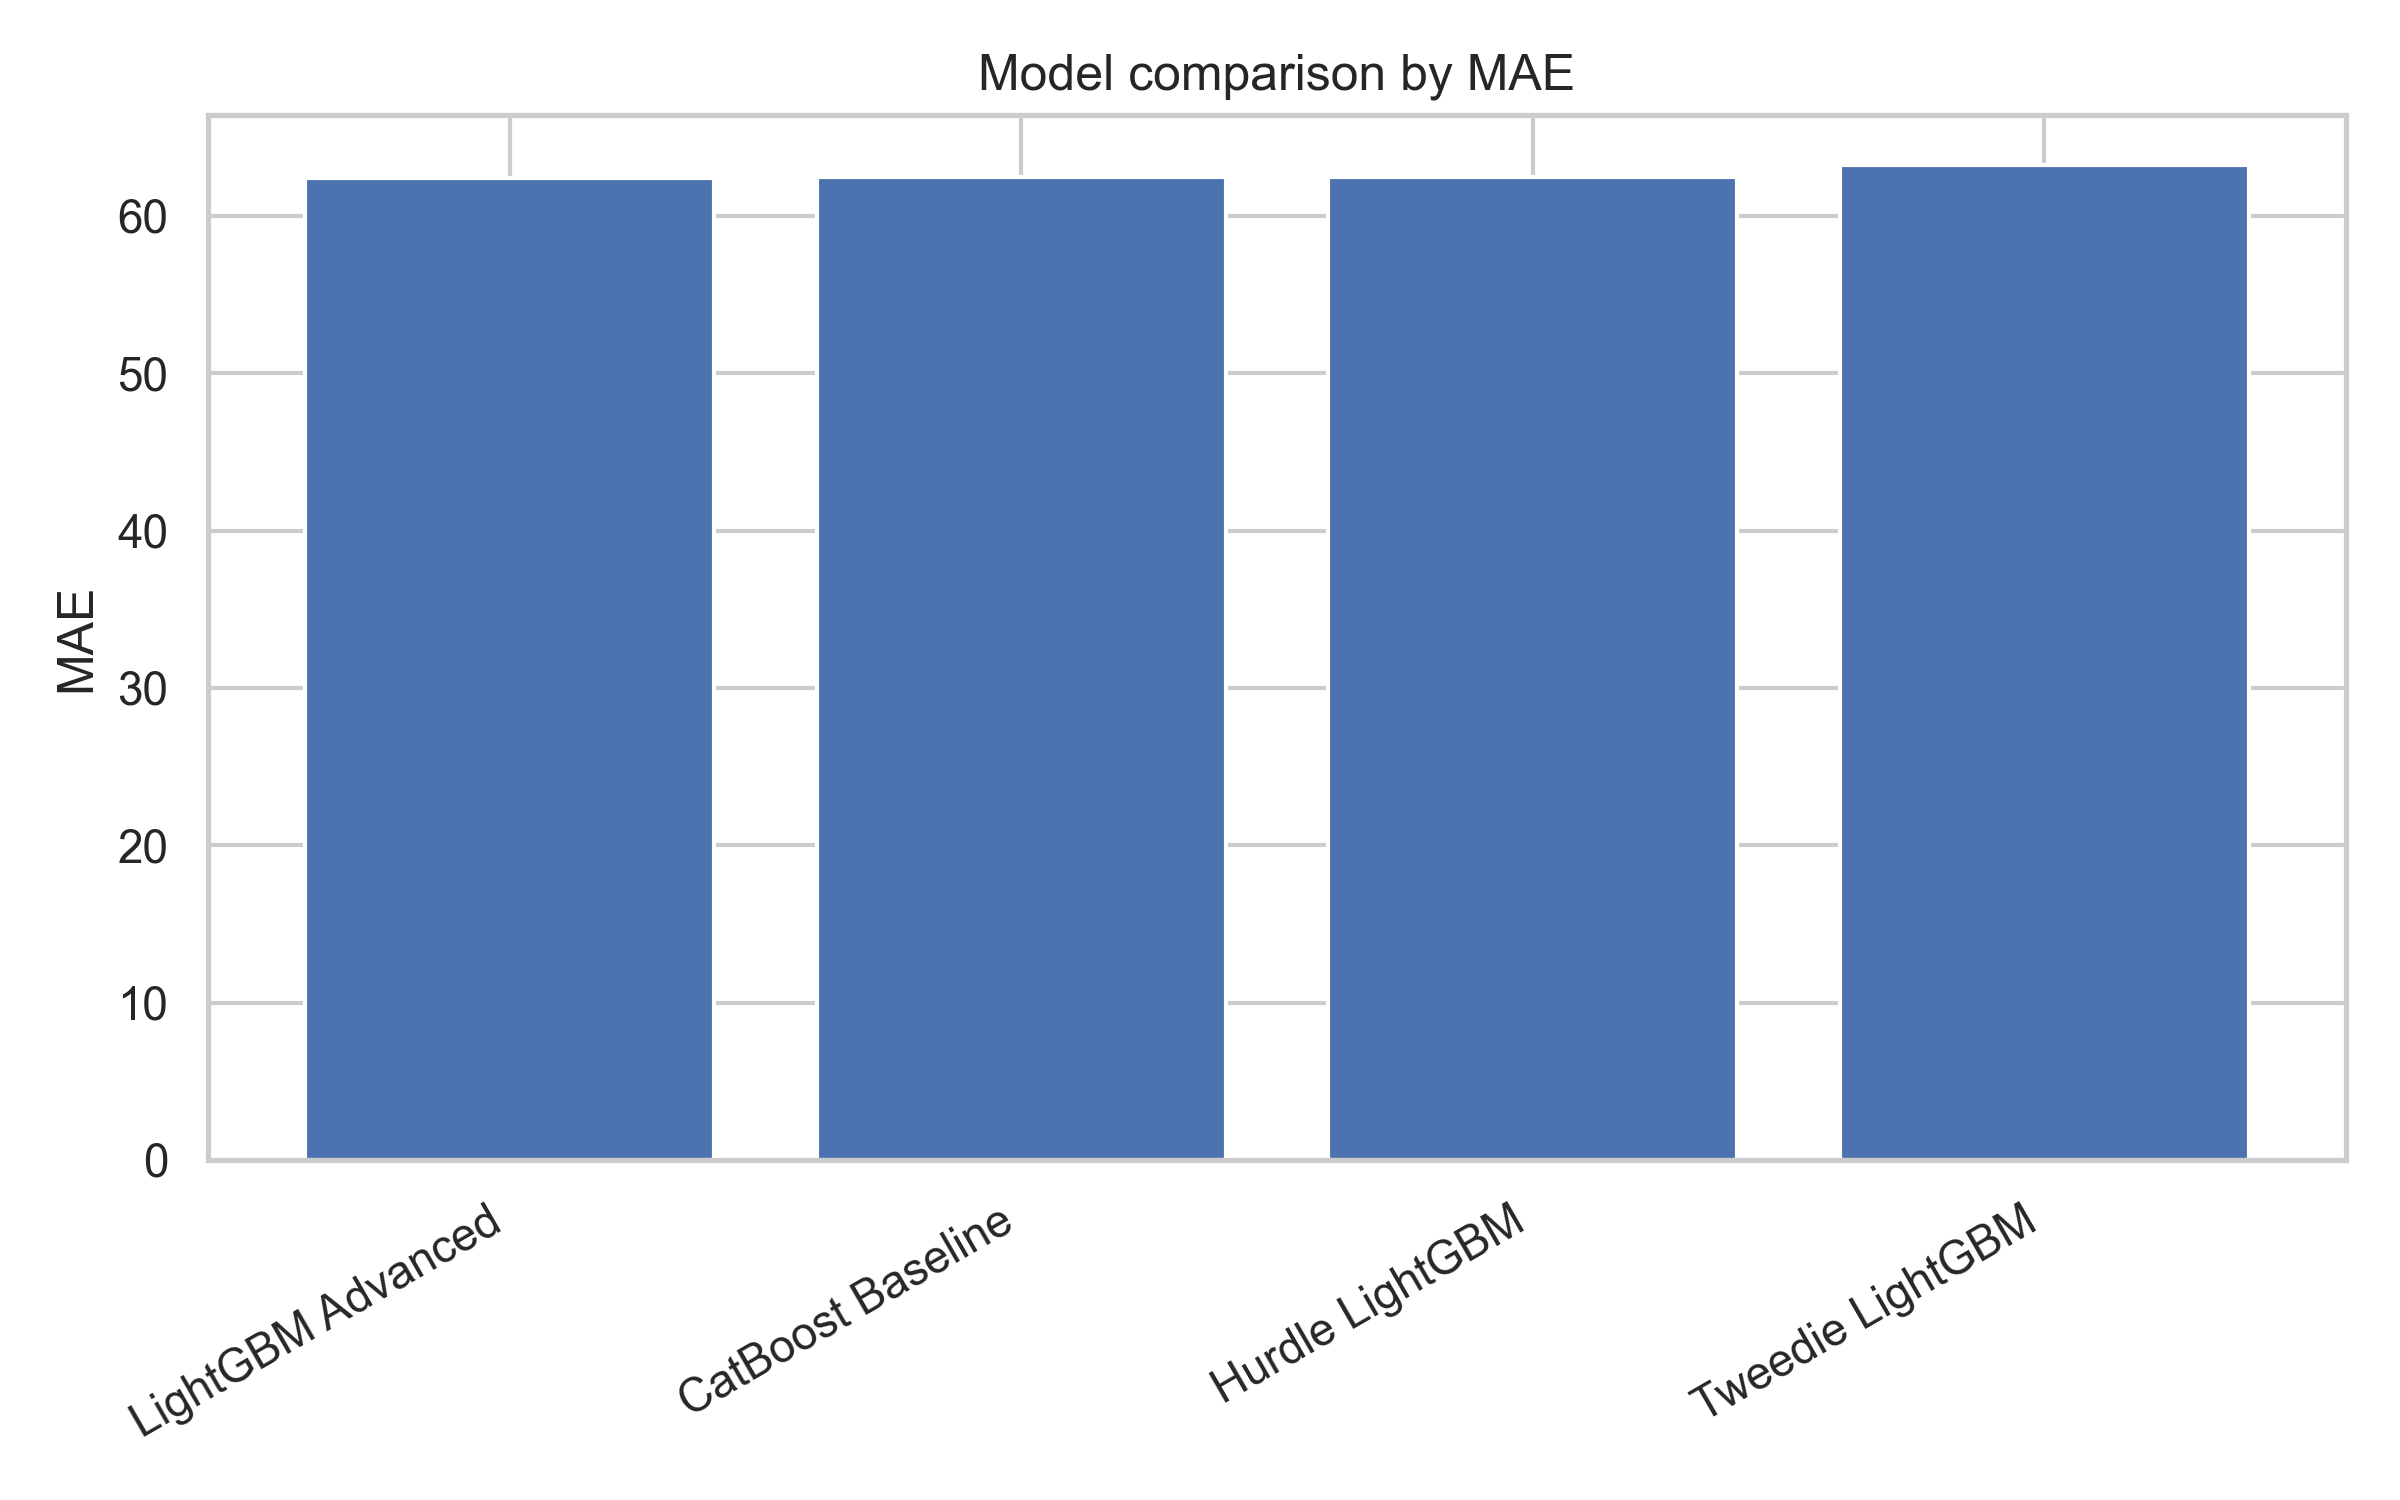
\includegraphics[width=\linewidth]{figures/7 model_mae_comparison.png}
\caption{MAE comparison bar plot.}
\end{figure}

\subsection{Ranking performance}
Spearman correlation was used to evaluate how well models ranked customers by expected revenue, which is particularly important in customer targeting applications. The advanced LightGBM and CatBoost models achieved the highest ranking performance. The Tweedie LightGBM achieved the weakest ranking performance, consistent with its conservative and zero-heavy prediction behaviour.

\begin{figure}[H]
\centering
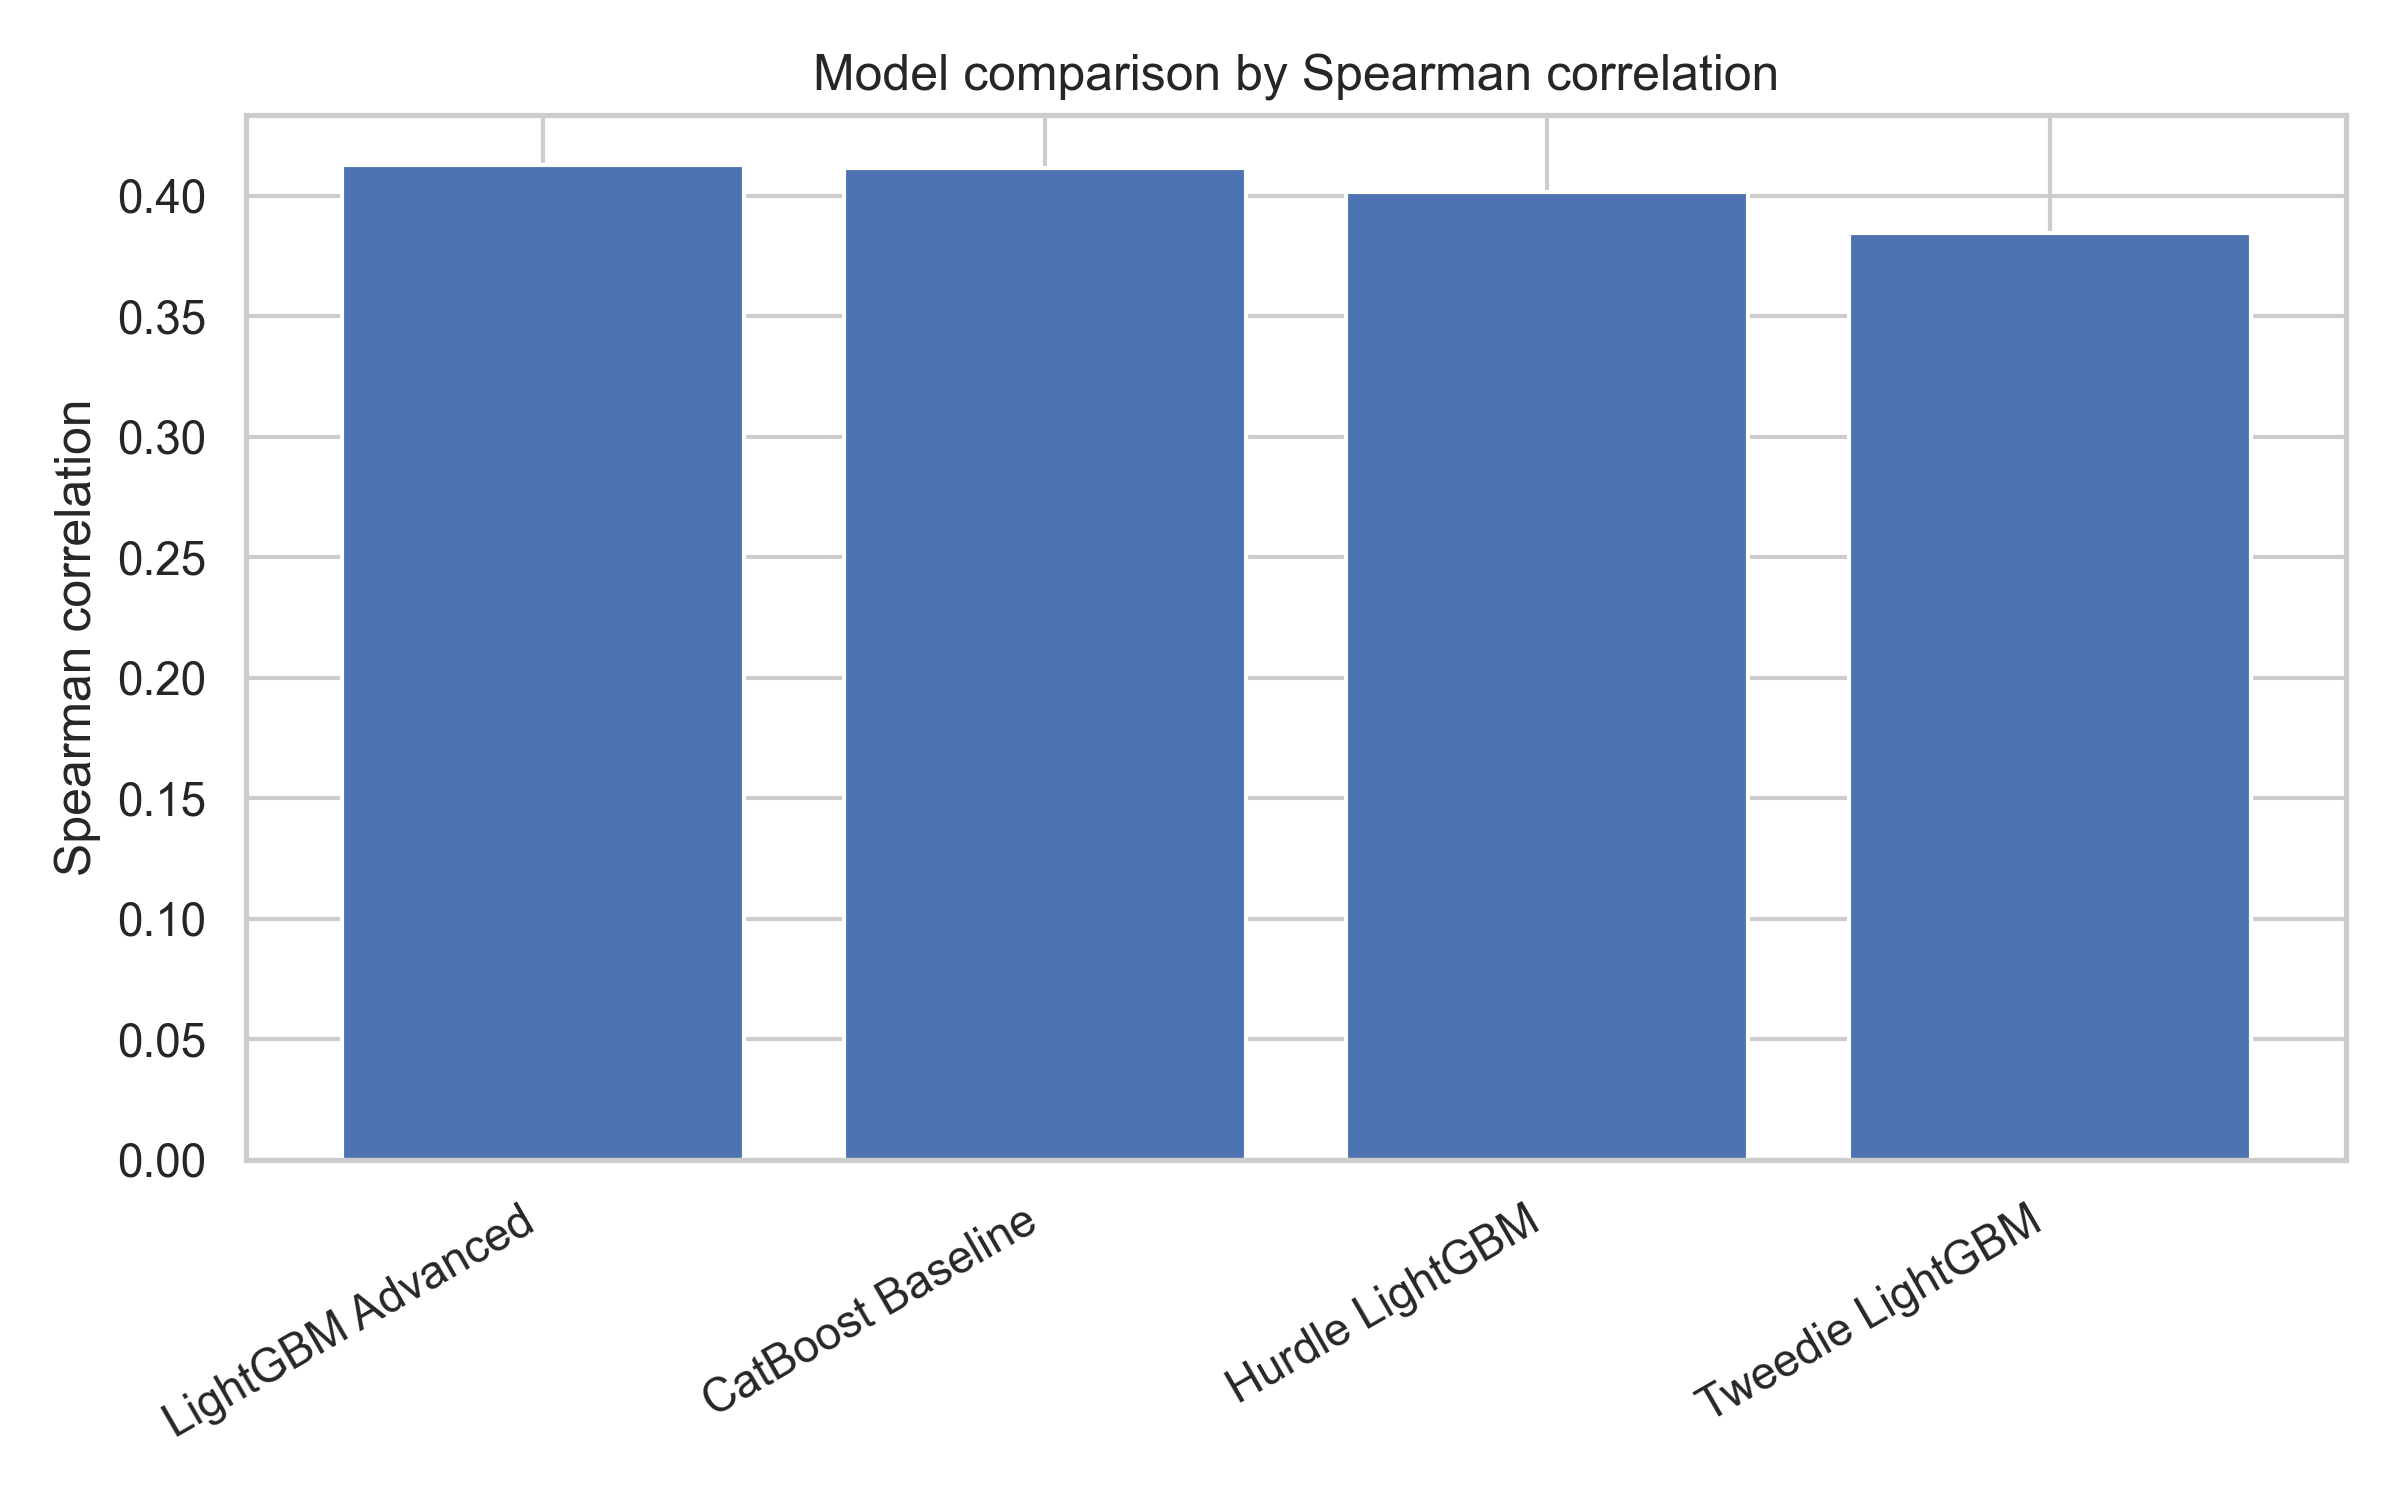
\includegraphics[width=\linewidth]{figures/8 model_spearman_comparison.png}
\caption{Spearman correlation comparison.}
\end{figure}

\subsection{Zero prediction behaviour}
Because the dataset contains a very large proportion of zero revenues, models faced a tradeoff between predicting many zeros and identifying positive spenders. Hurdle and Tweedie models predicted zeros much more aggressively than the standard boosting models. Experiments showed that higher zero prediction rates did not necessarily improve MAE, and the Tweedie model in particular overemphasised zero outcomes.

\begin{figure}[H]
\centering
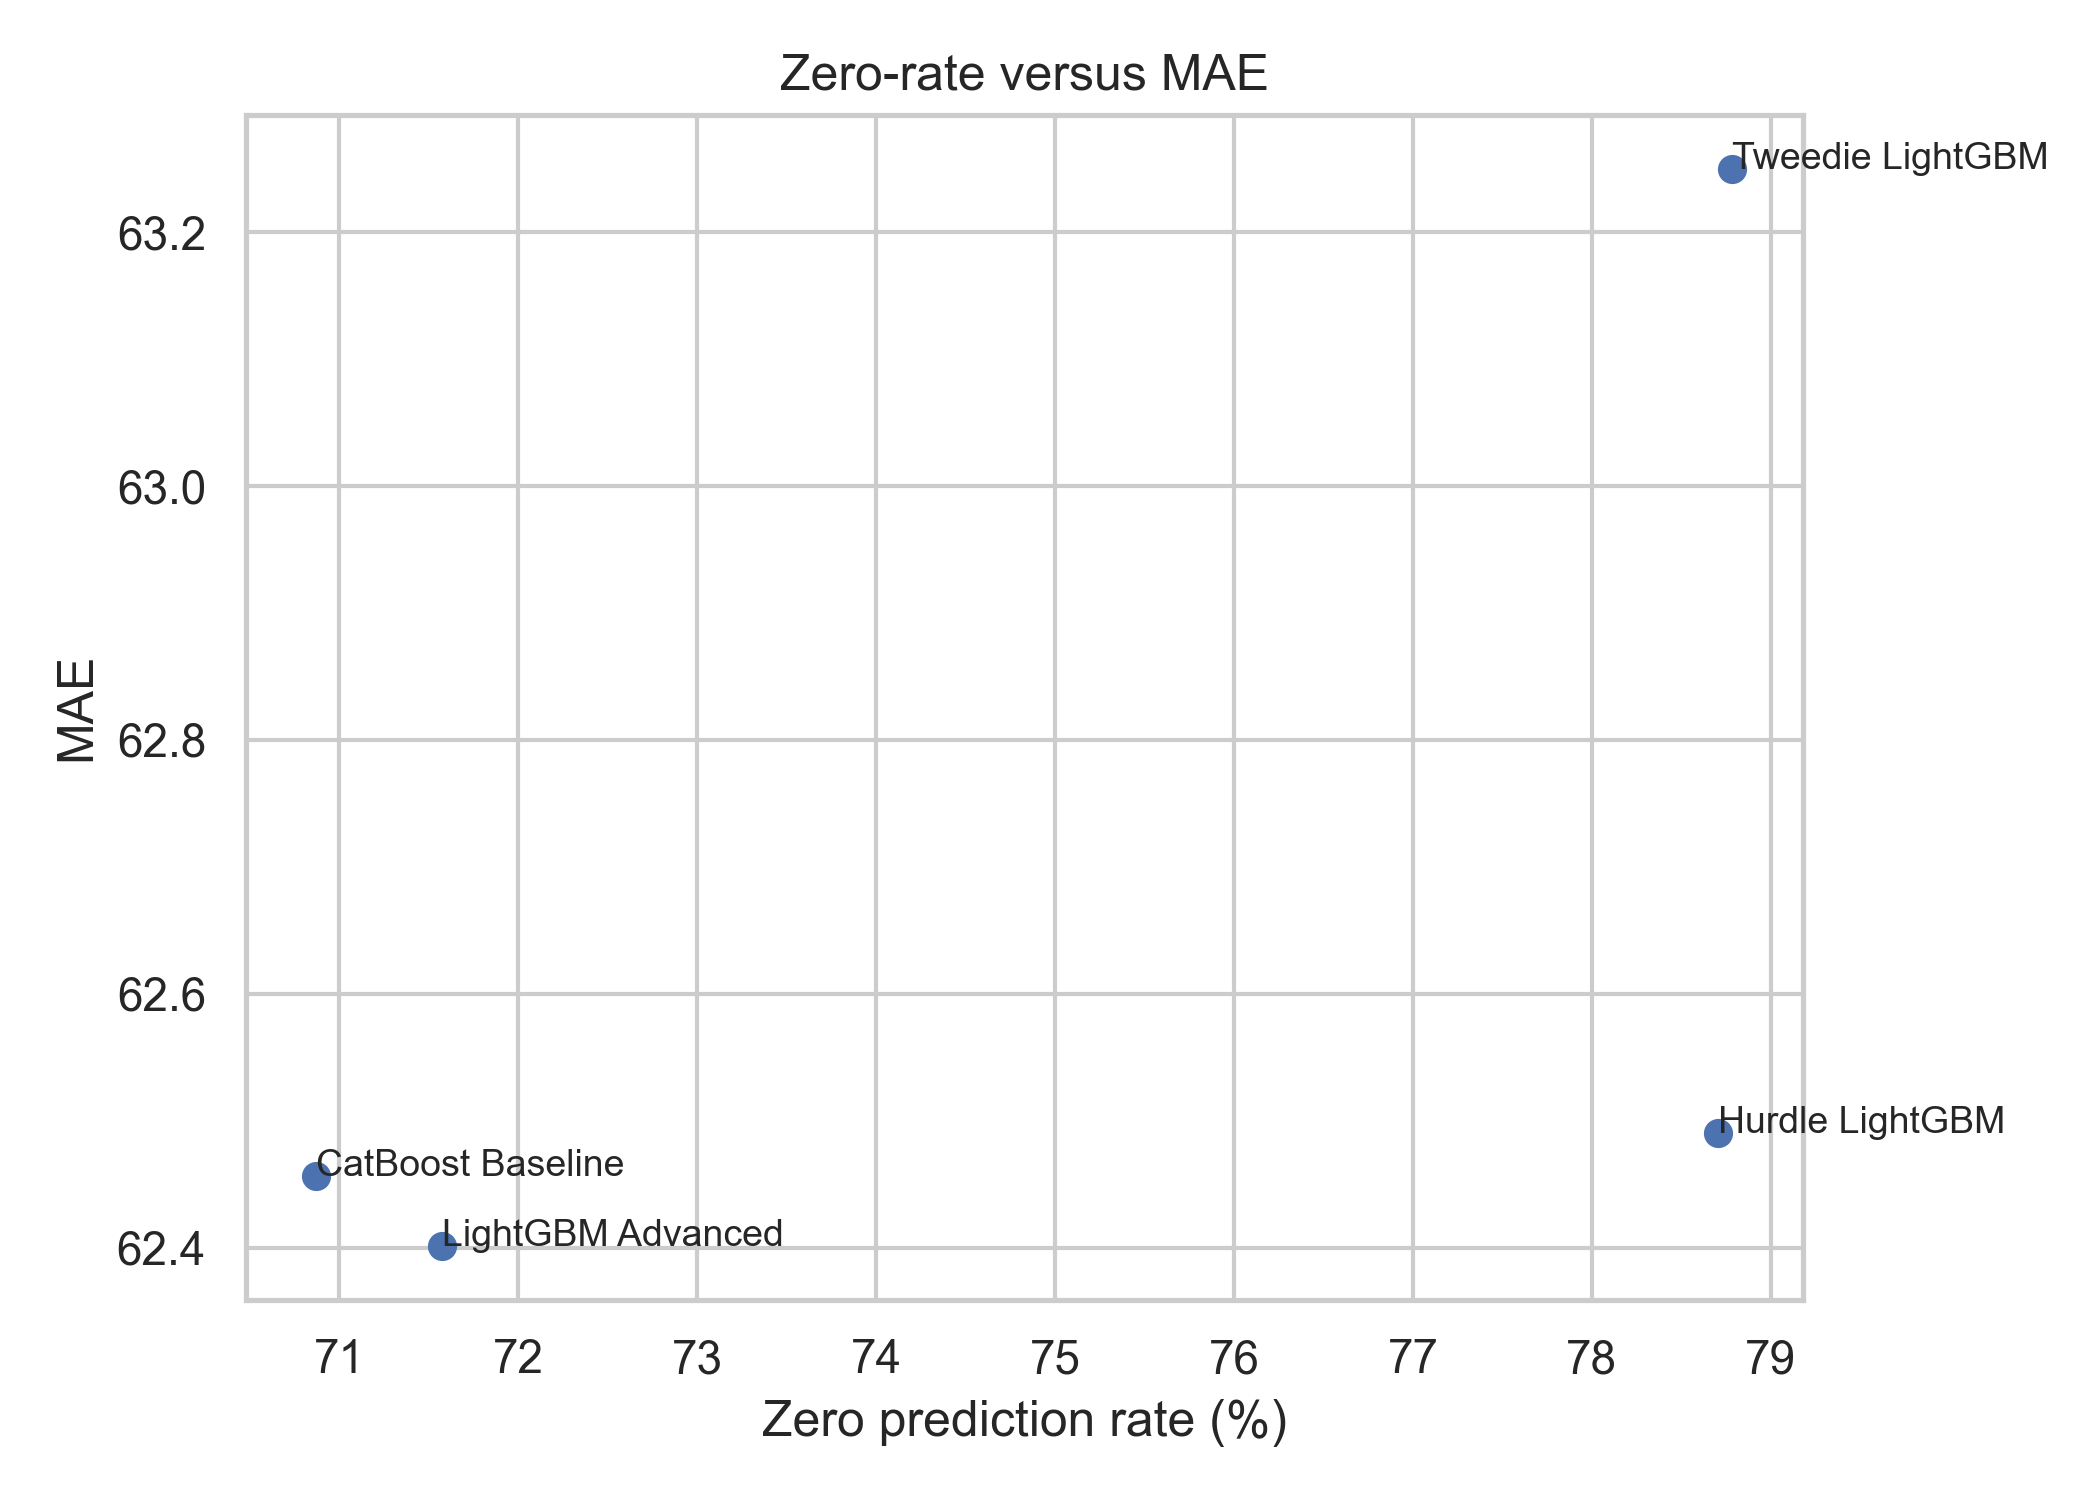
\includegraphics[width=\linewidth]{figures/9 zero_rate_vs_mae.png}
\caption{Zero-rate vs MAE plot.}
\end{figure}

\subsection{Similarity between model predictions}
Prediction correlations were analysed to determine whether different models learned substantially different structures. Most baseline boosting models produced highly similar prediction patterns, especially CatBoost, LightGBM and XGBoost. The Tweedie LightGBM model differed mainly because of its objective function rather than its architecture.

The standard LightGBM models optimised direct MAE/L1 loss, while the Tweedie model used LightGBM’s Tweedie objective with tweedie\_variance\_power equal to 1.2. The Tweedie objective is designed for zero-inflated positive targets and assumes a compound Poisson-Gamma type distribution. This encourages the model to treat zero outcomes and positive spending behaviour differently. Although Tweedie achieved weaker standalone MAE, its calibration behaviour differed from the other LightGBM variants, suggesting that it captured somewhat different zero-inflation structure. Such diversity can still be useful in larger ensembles even when standalone accuracy is lower.


\begin{figure}[H]
\centering
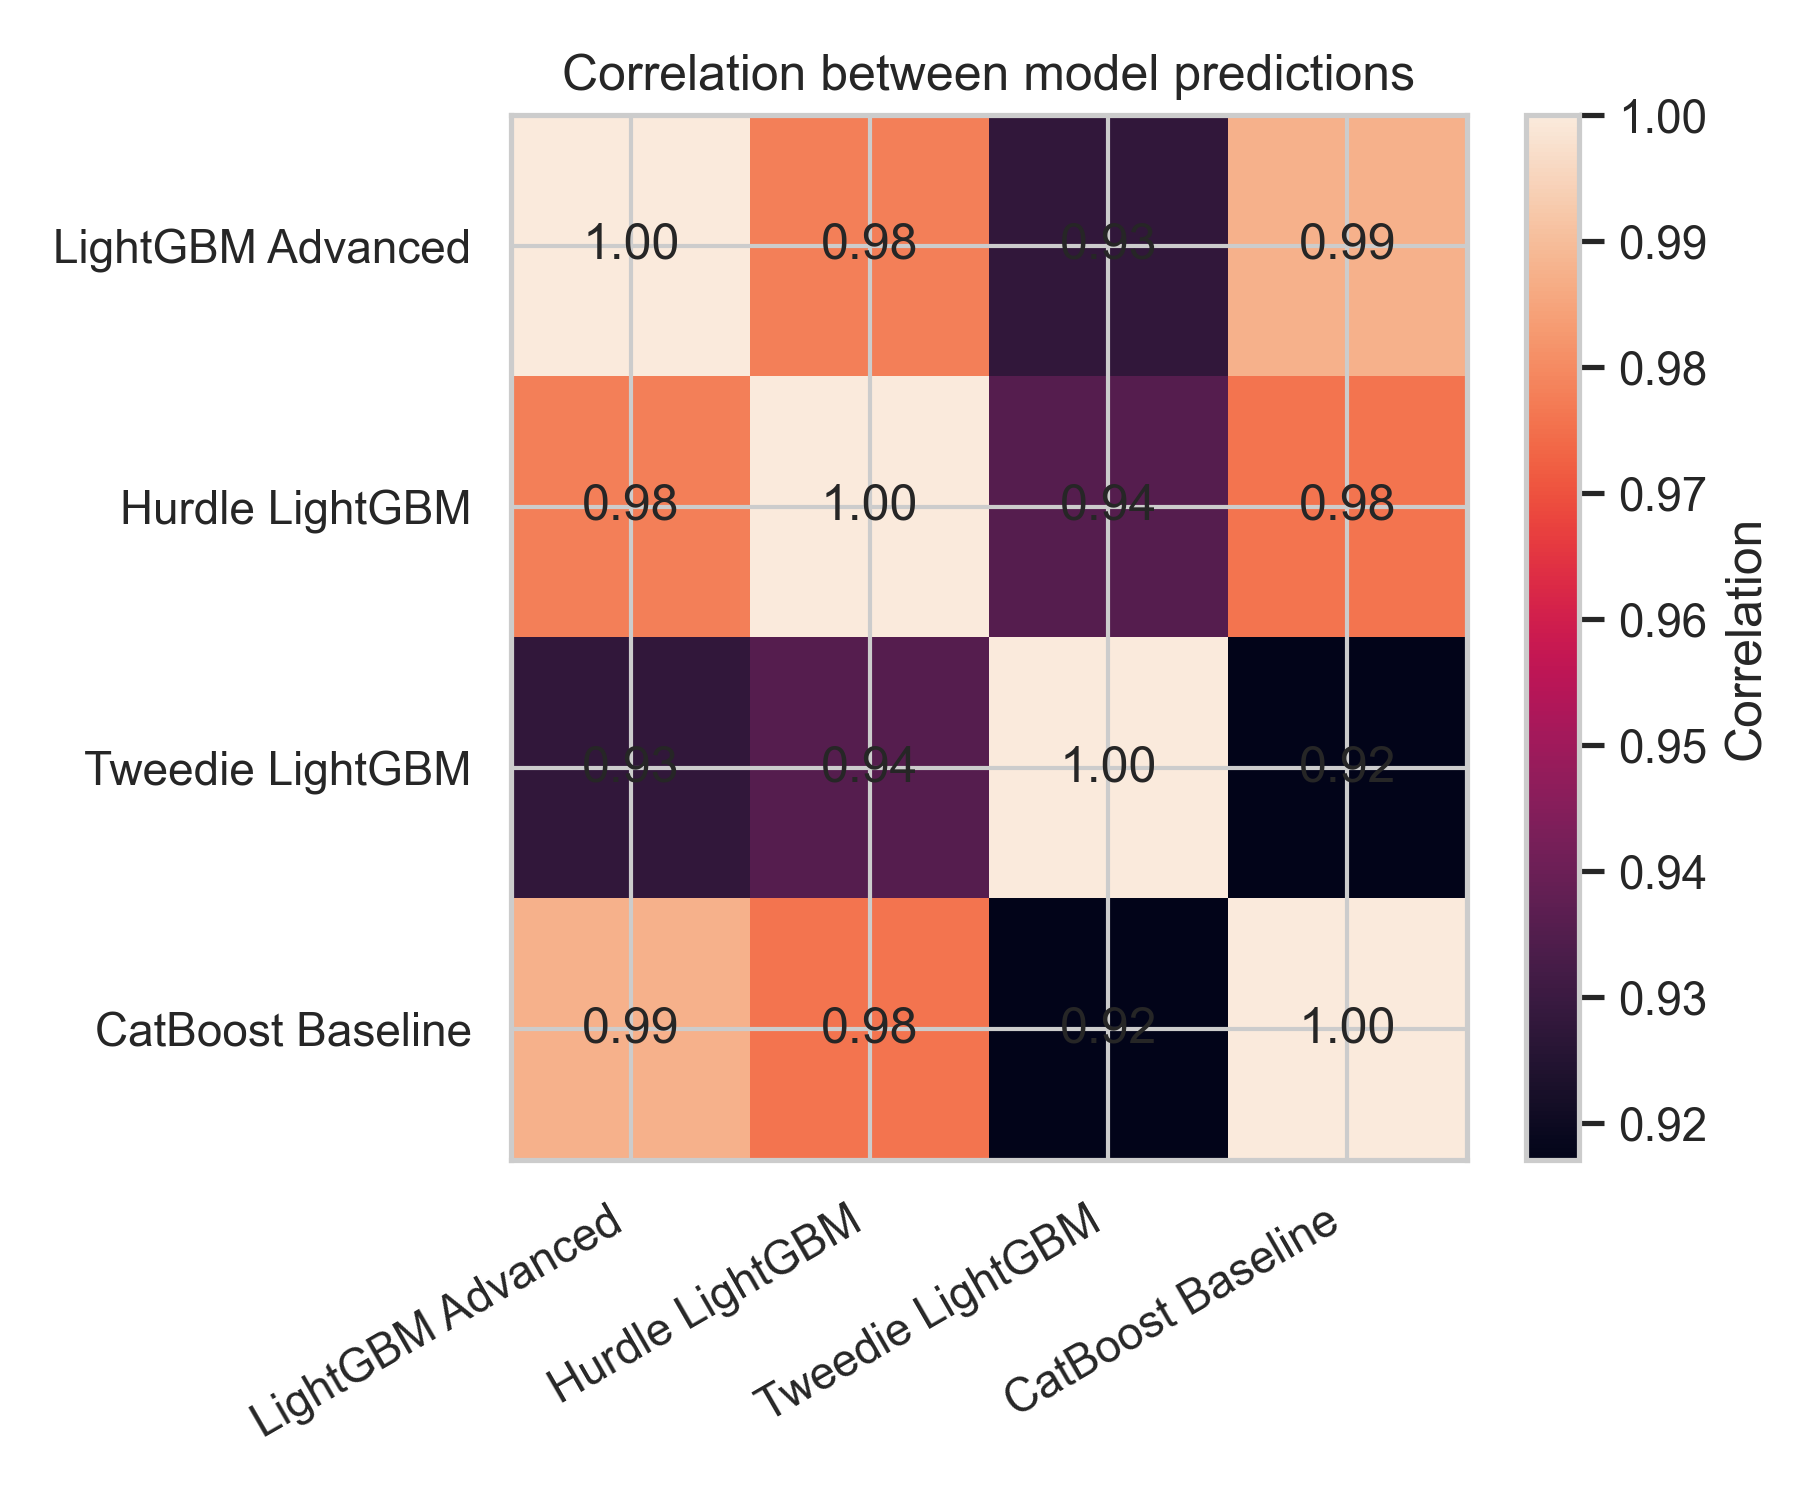
\includegraphics[width=\linewidth]{figures/10 model_prediction_correlation_heatmap.png}
\caption{Prediction correlation heatmap.}
\end{figure}

\subsection{Calibration analysis}
The combined calibration plot compares the actual average revenue with the predicted average revenue across prediction deciles. The black dashed line represents the actual average revenue in each decile, while the coloured lines represent the predicted average revenue of the different models. All models followed the same general pattern: predicted revenue remained low in the lower and middle deciles and rose sharply in the highest deciles, indicating that models primarily identified high-value customers in the upper prediction range.

However, all models strongly underpredicted the actual revenue in the highest decile, confirming that the models were conservative for large spenders. This is expected given the skewed target distribution and the use of MAE-based training. The advanced LightGBM, Hurdle LightGBM, and XGBoost predictions followed a broadly similar shape, while the Tweedie LightGBM remained more conservative across much of the calibration curve. Overall, the plot was most useful for showing general underprediction of high-value customers, but was less informative for detailed model-by-model comparison because the prediction curves overlapped strongly.

\begin{figure}[H]
\centering
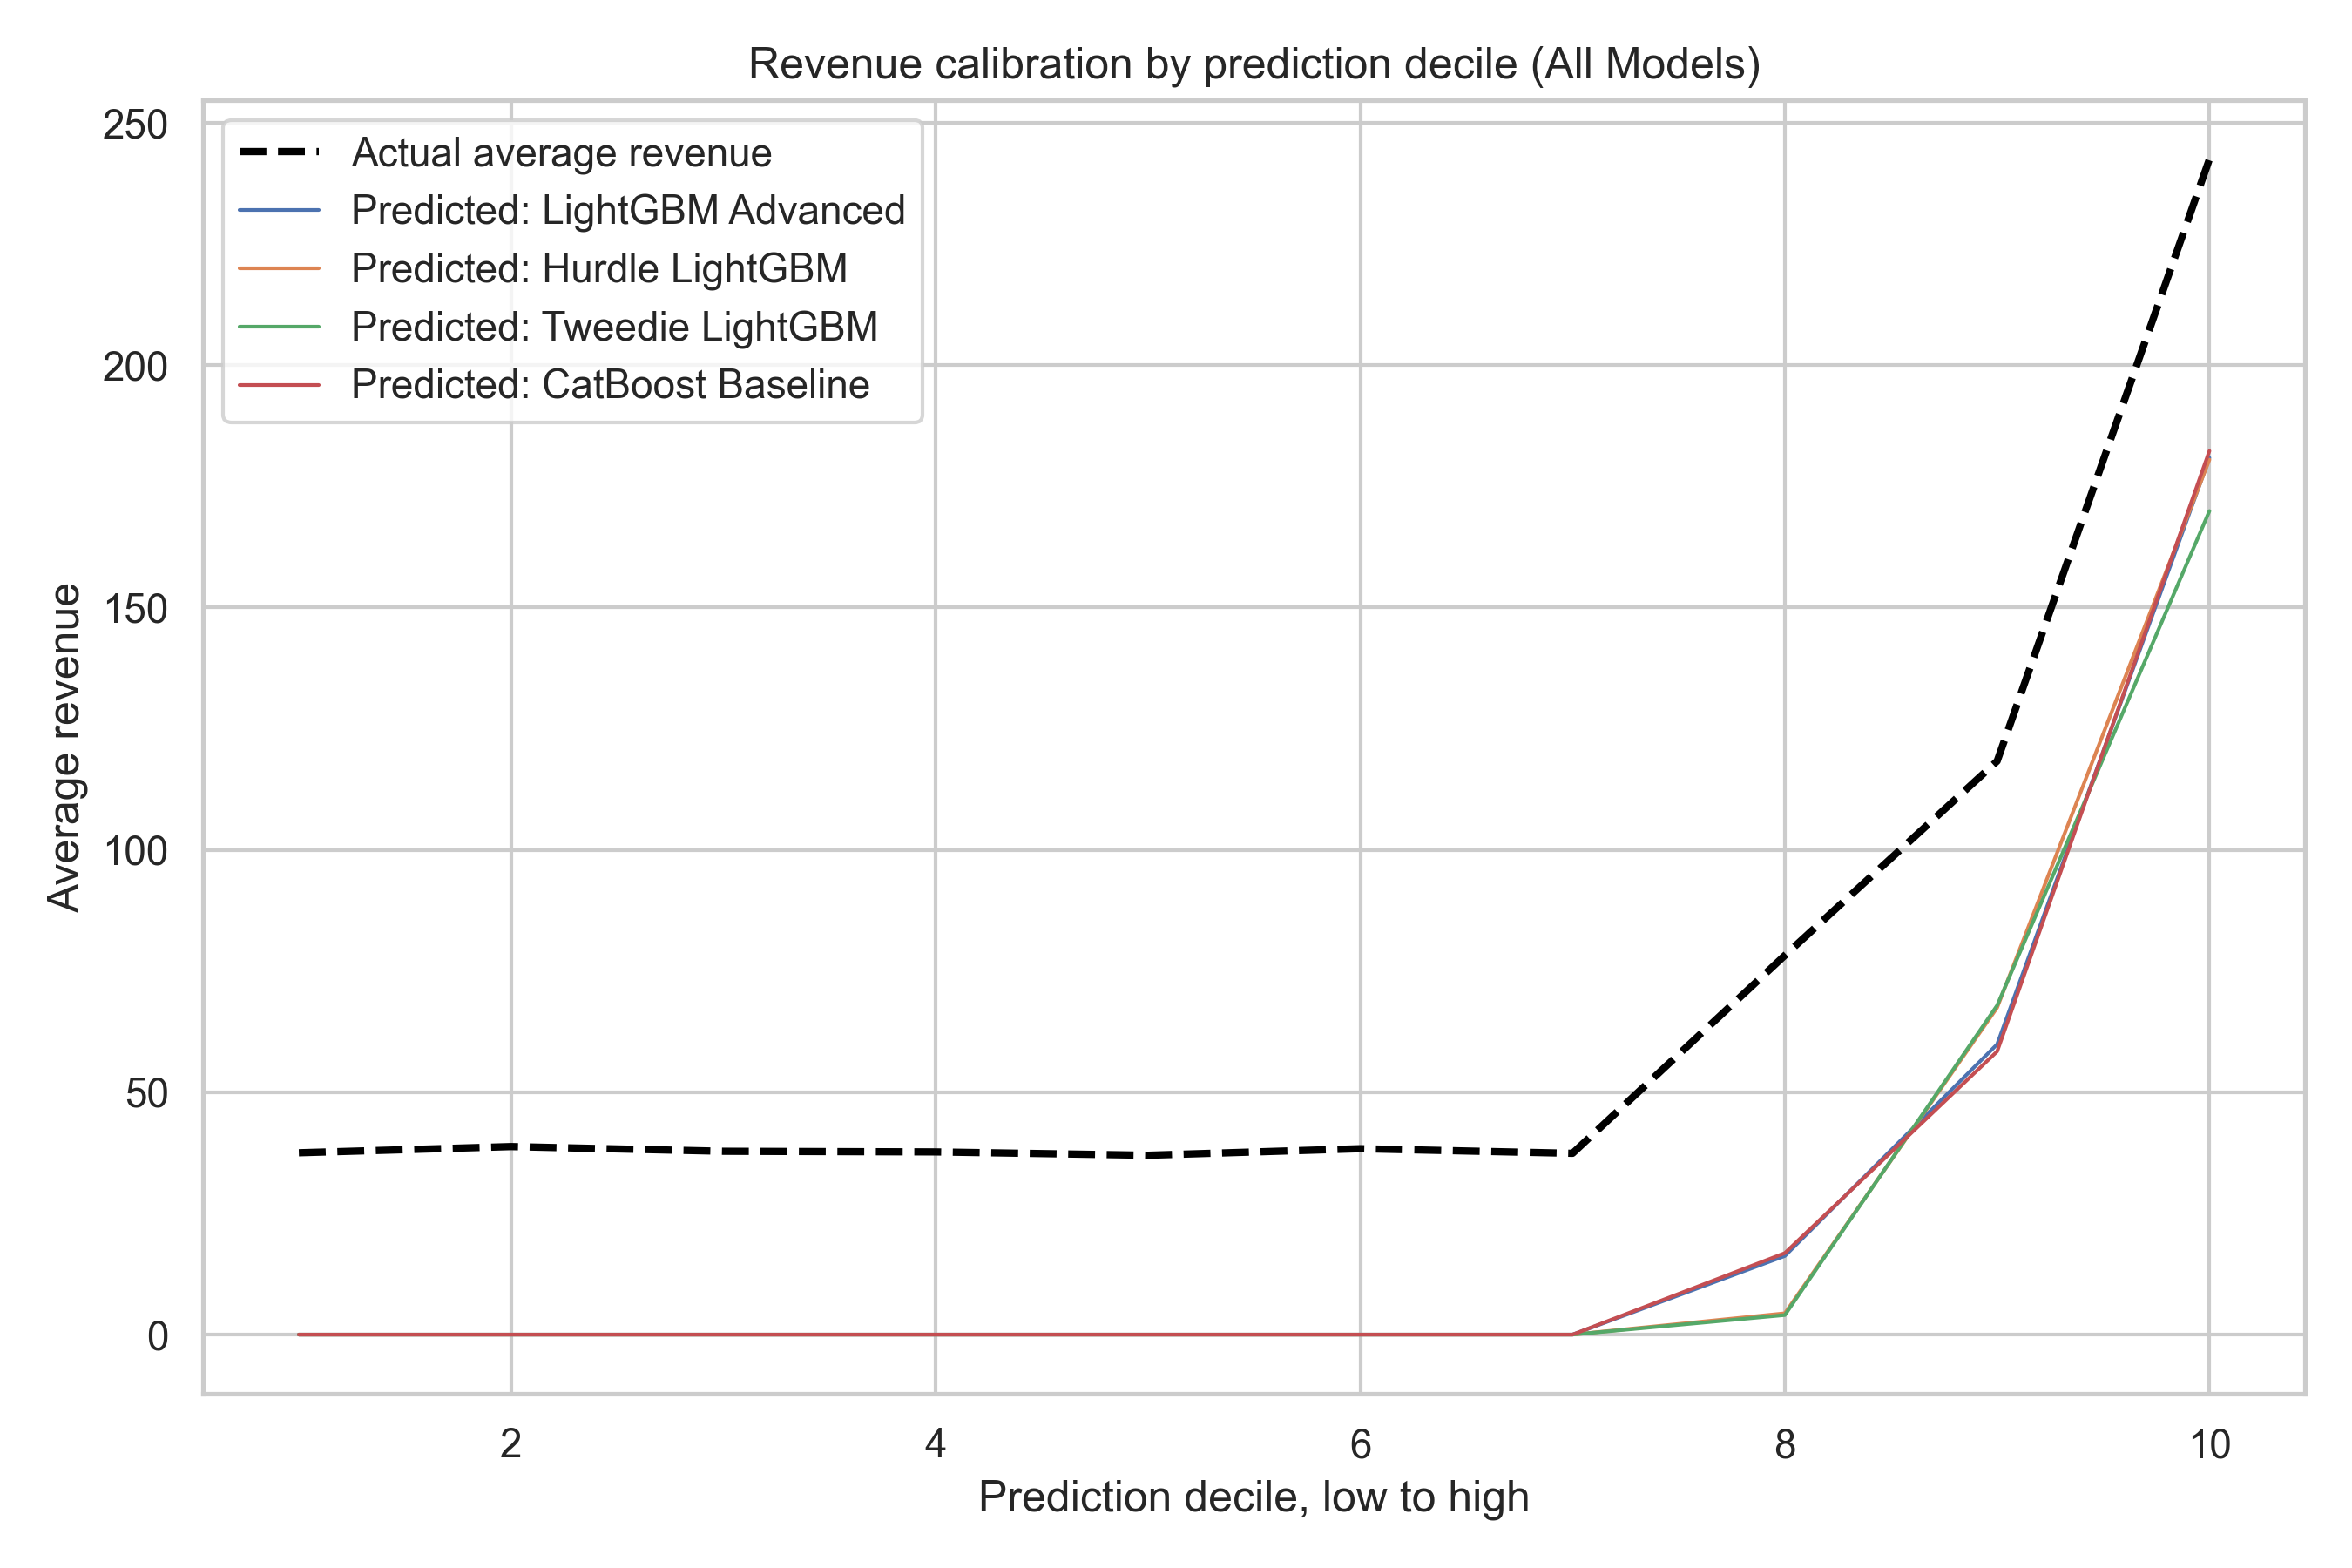
\includegraphics[width=\linewidth]{figures/11 calibration_deciles_all_models.png}
\caption{Calibration plot.}
\end{figure}

\subsection{Predicted versus actual revenue analysis}
Scatterplots of log-transformed predictions versus realised revenue were analysed using samples of 1,000 predictions. The diagonal line represented perfect prediction accuracy, while annotations counted correctly predicted zeros, false positives and false negatives. CatBoost captured the general positive relationship between predicted and actual revenue, although many positive spenders were still predicted as zero and predictions for very large revenues were compressed. The LightGBM baseline produced a slightly smoother prediction spread and maintained reasonable alignment with the diagonal, although zero prediction remained substantial. XGBoost showed greater dispersion and somewhat less stable calibration, including visible extreme underpredictions.
The Hurdle LightGBM model predicted many more exact zeros. This improved sparsity modelling but also increased the number of false negative spenders, with many positive revenues collapsed towards zero predictions. Advanced LightGBM showed slightly improved alignment with the diagonal and better separation of positive-revenue customers, while maintaining a balanced prediction spread. Tweedie LightGBM produced predictions concentrated around moderate values and predicted zeros aggressively, which likely contributed to weaker accuracy.

\begin{figure}[H]
\centering
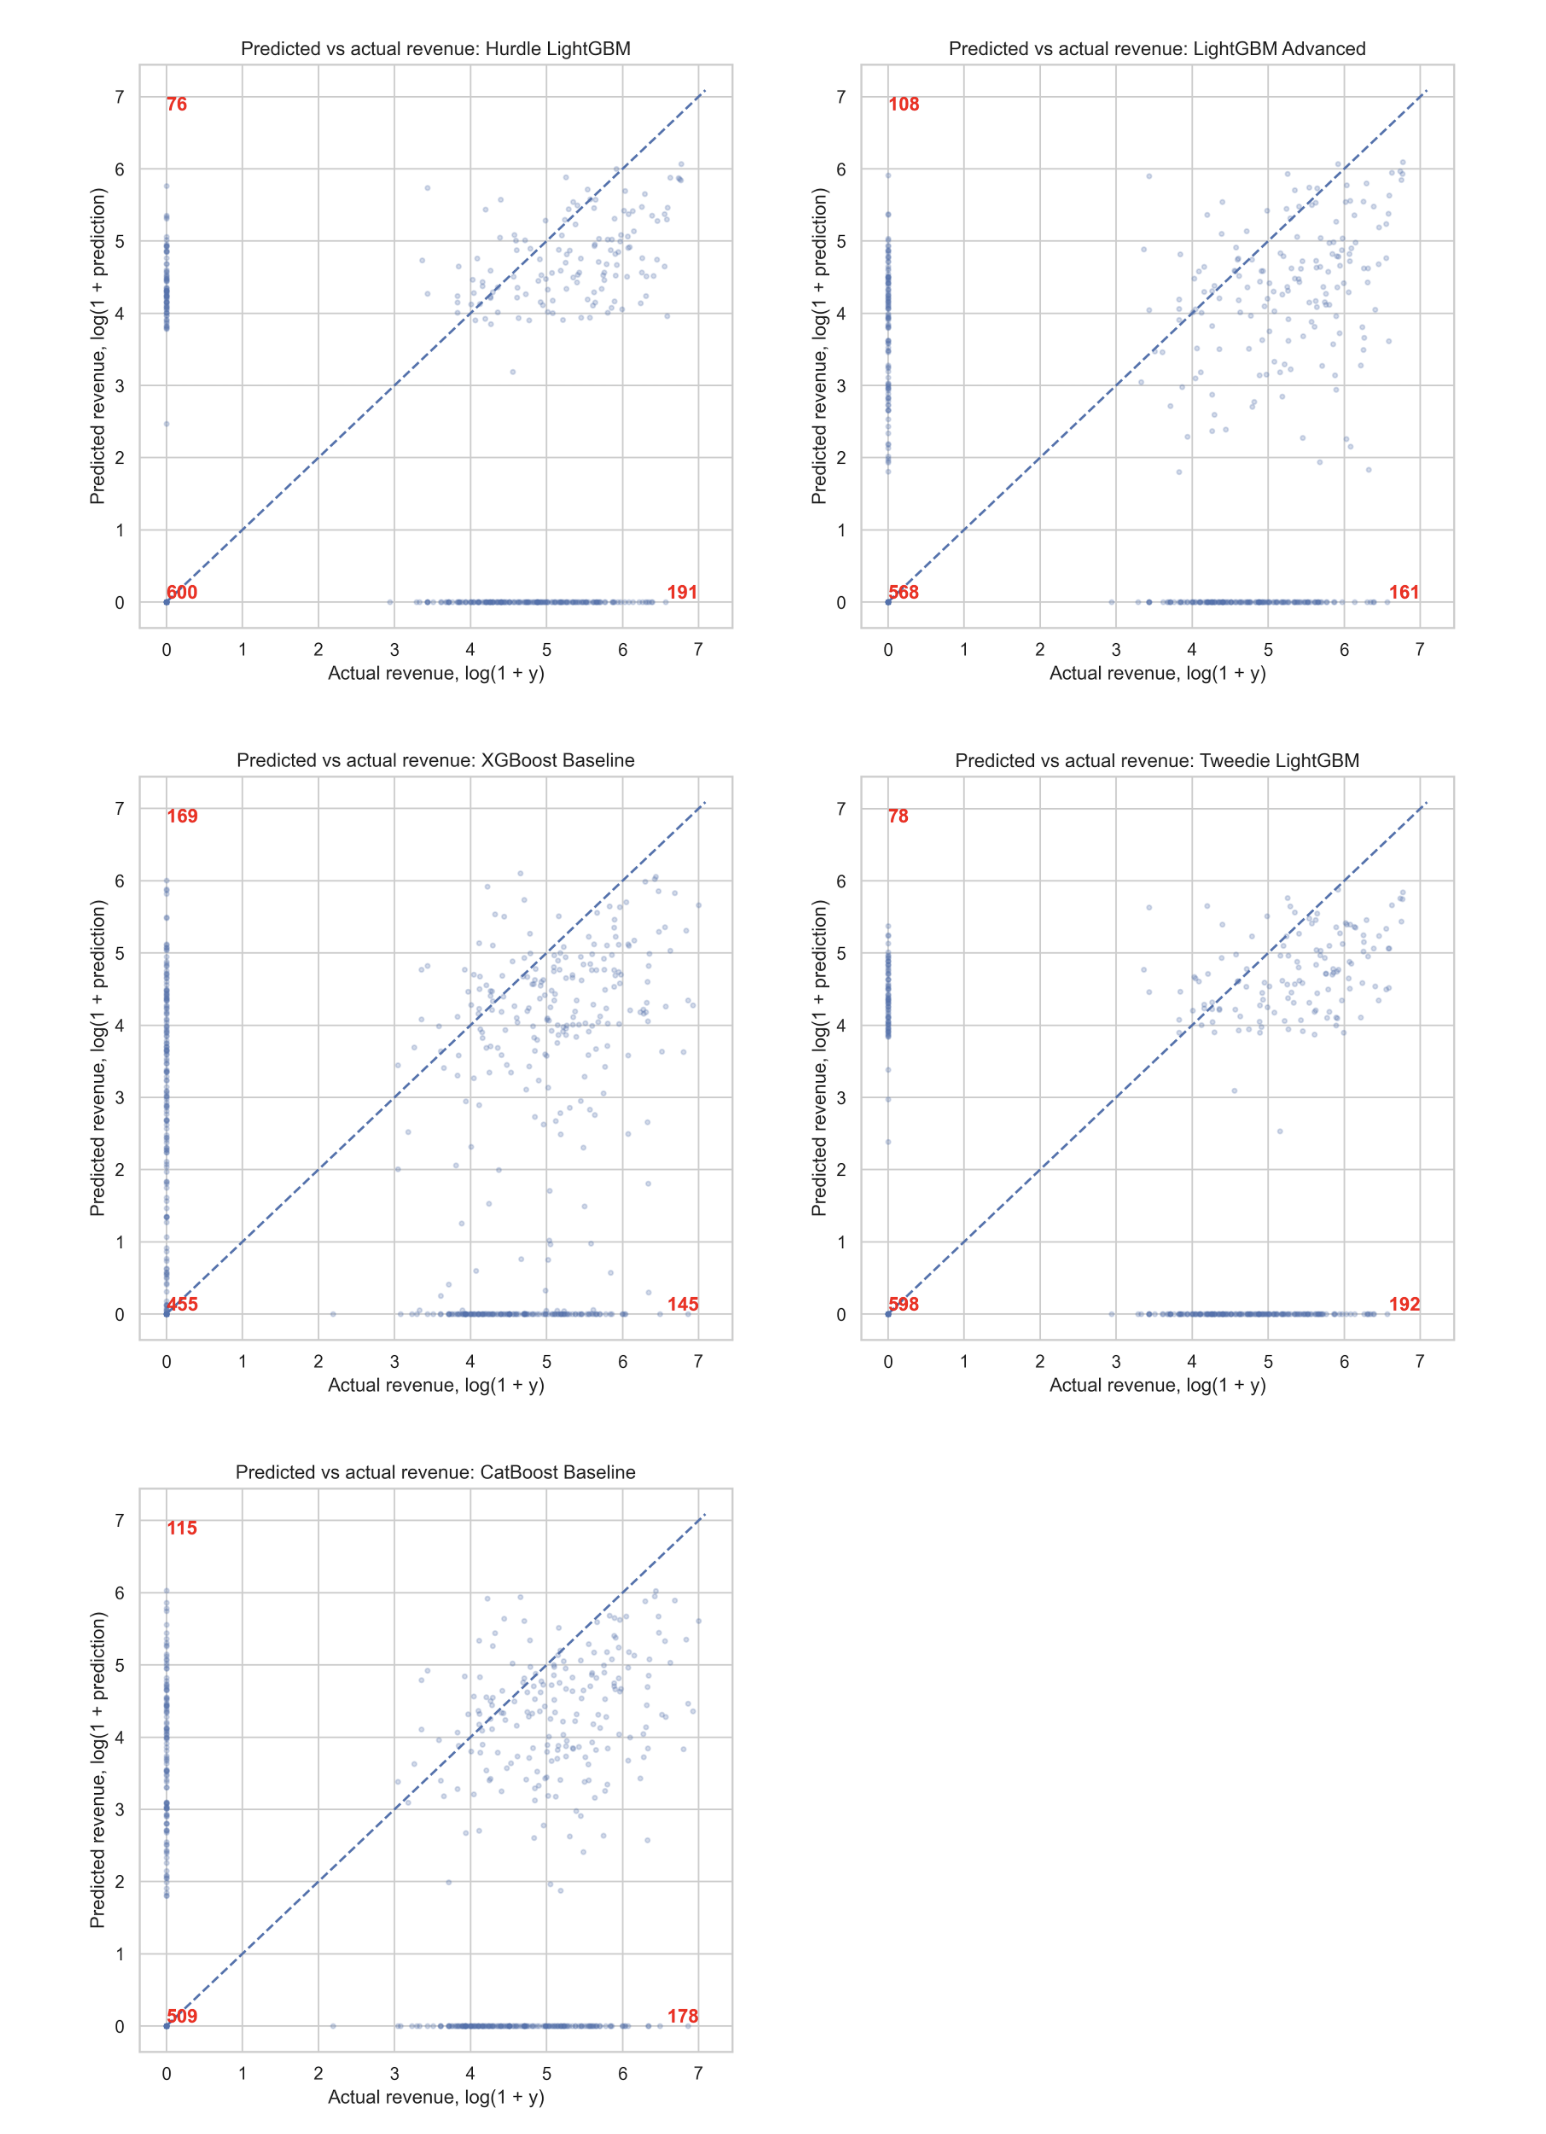
\includegraphics[width=\linewidth]{figures/12 predicted_vs_actual_revenue_analysis.png}
\caption{Predicted vs actual revenue scatterplots.}
\end{figure}

\subsection{Residual analysis}
Residual distributions were compared across all models. Most models produced similar residual spread, and large revenues remained difficult to predict accurately due to the highly skewed target distribution. Residual boxplots showed relatively similar error distributions across models, with most models slightly underpredicting very large revenues. Extreme positive residuals remained present for all approaches.

\begin{figure}[H]
\centering
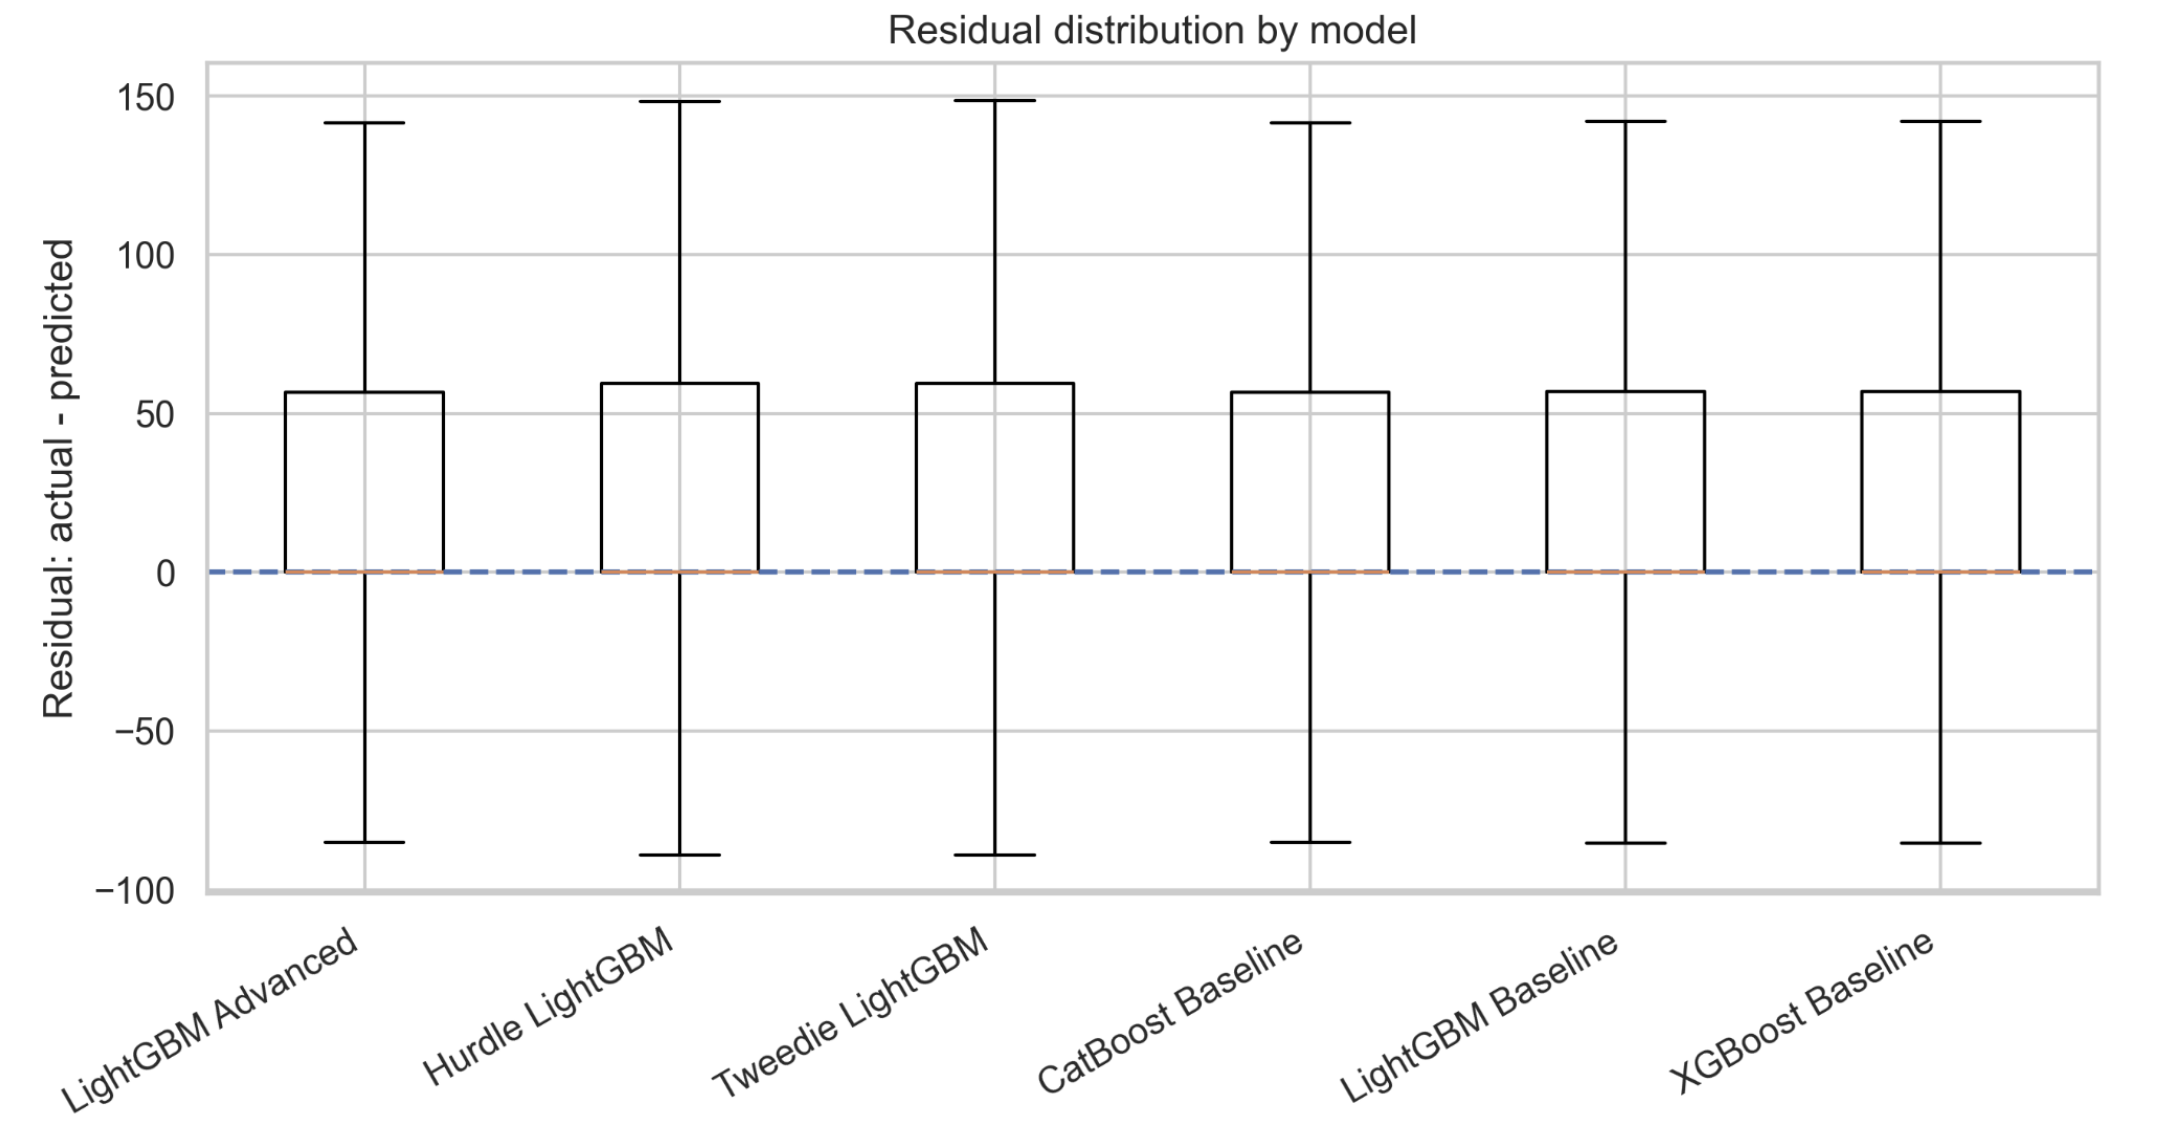
\includegraphics[width=\linewidth]{figures/13 residual analysis.png}
\caption{Residual boxplots.}
\end{figure}

\subsection{Final conclusions}
The advanced LightGBM model achieved the best balance between calibration, ranking ability, and overall prediction accuracy. Baseline boosting models already performed strongly, indicating that tree-based methods are highly suitable for this customer revenue prediction task. More specialised zero-inflated approaches such as hurdle and Tweedie models did not substantially improve performance on this dataset.

\subsection{Discussion and conclusions}
The experiments showed that recency, spending stability, returns and customer activity consistently had a large impact on predictive performance. Feature engineering was especially important: improvements in feature construction often produced larger gains than small hyperparameter changes. Gradient boosting tree models outperformed simpler approaches because the relationship between historical behaviour and future revenue was non-linear.
LightGBM emerged as the strongest model family. The combination of behavioural feature engineering, MAE optimisation and conservative regularisation produced the most stable results. Hurdle and Tweedie approaches were theoretically attractive because of the zero-inflated target, but they did not outperform direct MAE-based boosting. Ensembles improved robustness slightly, although the best standalone LightGBM model remained marginally superior. Post-processing helped when behavioural adjustments were moderate, but overly aggressive filtering removed useful positive signal and worsened MAE.


\section{Model interpretation}
This section examines which customer characteristics drive the predictions of the best LightGBM models. Several complementary interpretation techniques were used, including LightGBM gain importance, LightGBM split importance, permutation importance, PCA analysis, and t-SNE customer segmentation.

\subsection{Lightgbm gain importance}
The LightGBM gain importance plot shows which variables contributed most strongly to reducing prediction error during tree construction. The most important feature was favorite\_brand\_encoded, with a normalised gain importance of approximately 21.7 percent. This suggests that customer brand preference contains substantial predictive information about future revenue behaviour. Other highly important features included n\_orders, favorite\_brand\_freq, revenue\_std, recency\_days, and customer\_lifetime\_days. This indicates that both behavioural activity variables and historical spending variability strongly influence model predictions. The high importance of recency\_days confirms that customer inactivity is one of the strongest indicators of reduced future revenue, and the importance of revenue\_std suggests that spending consistency and volatility also help separate customer types.

\begin{figure}[H]
\centering
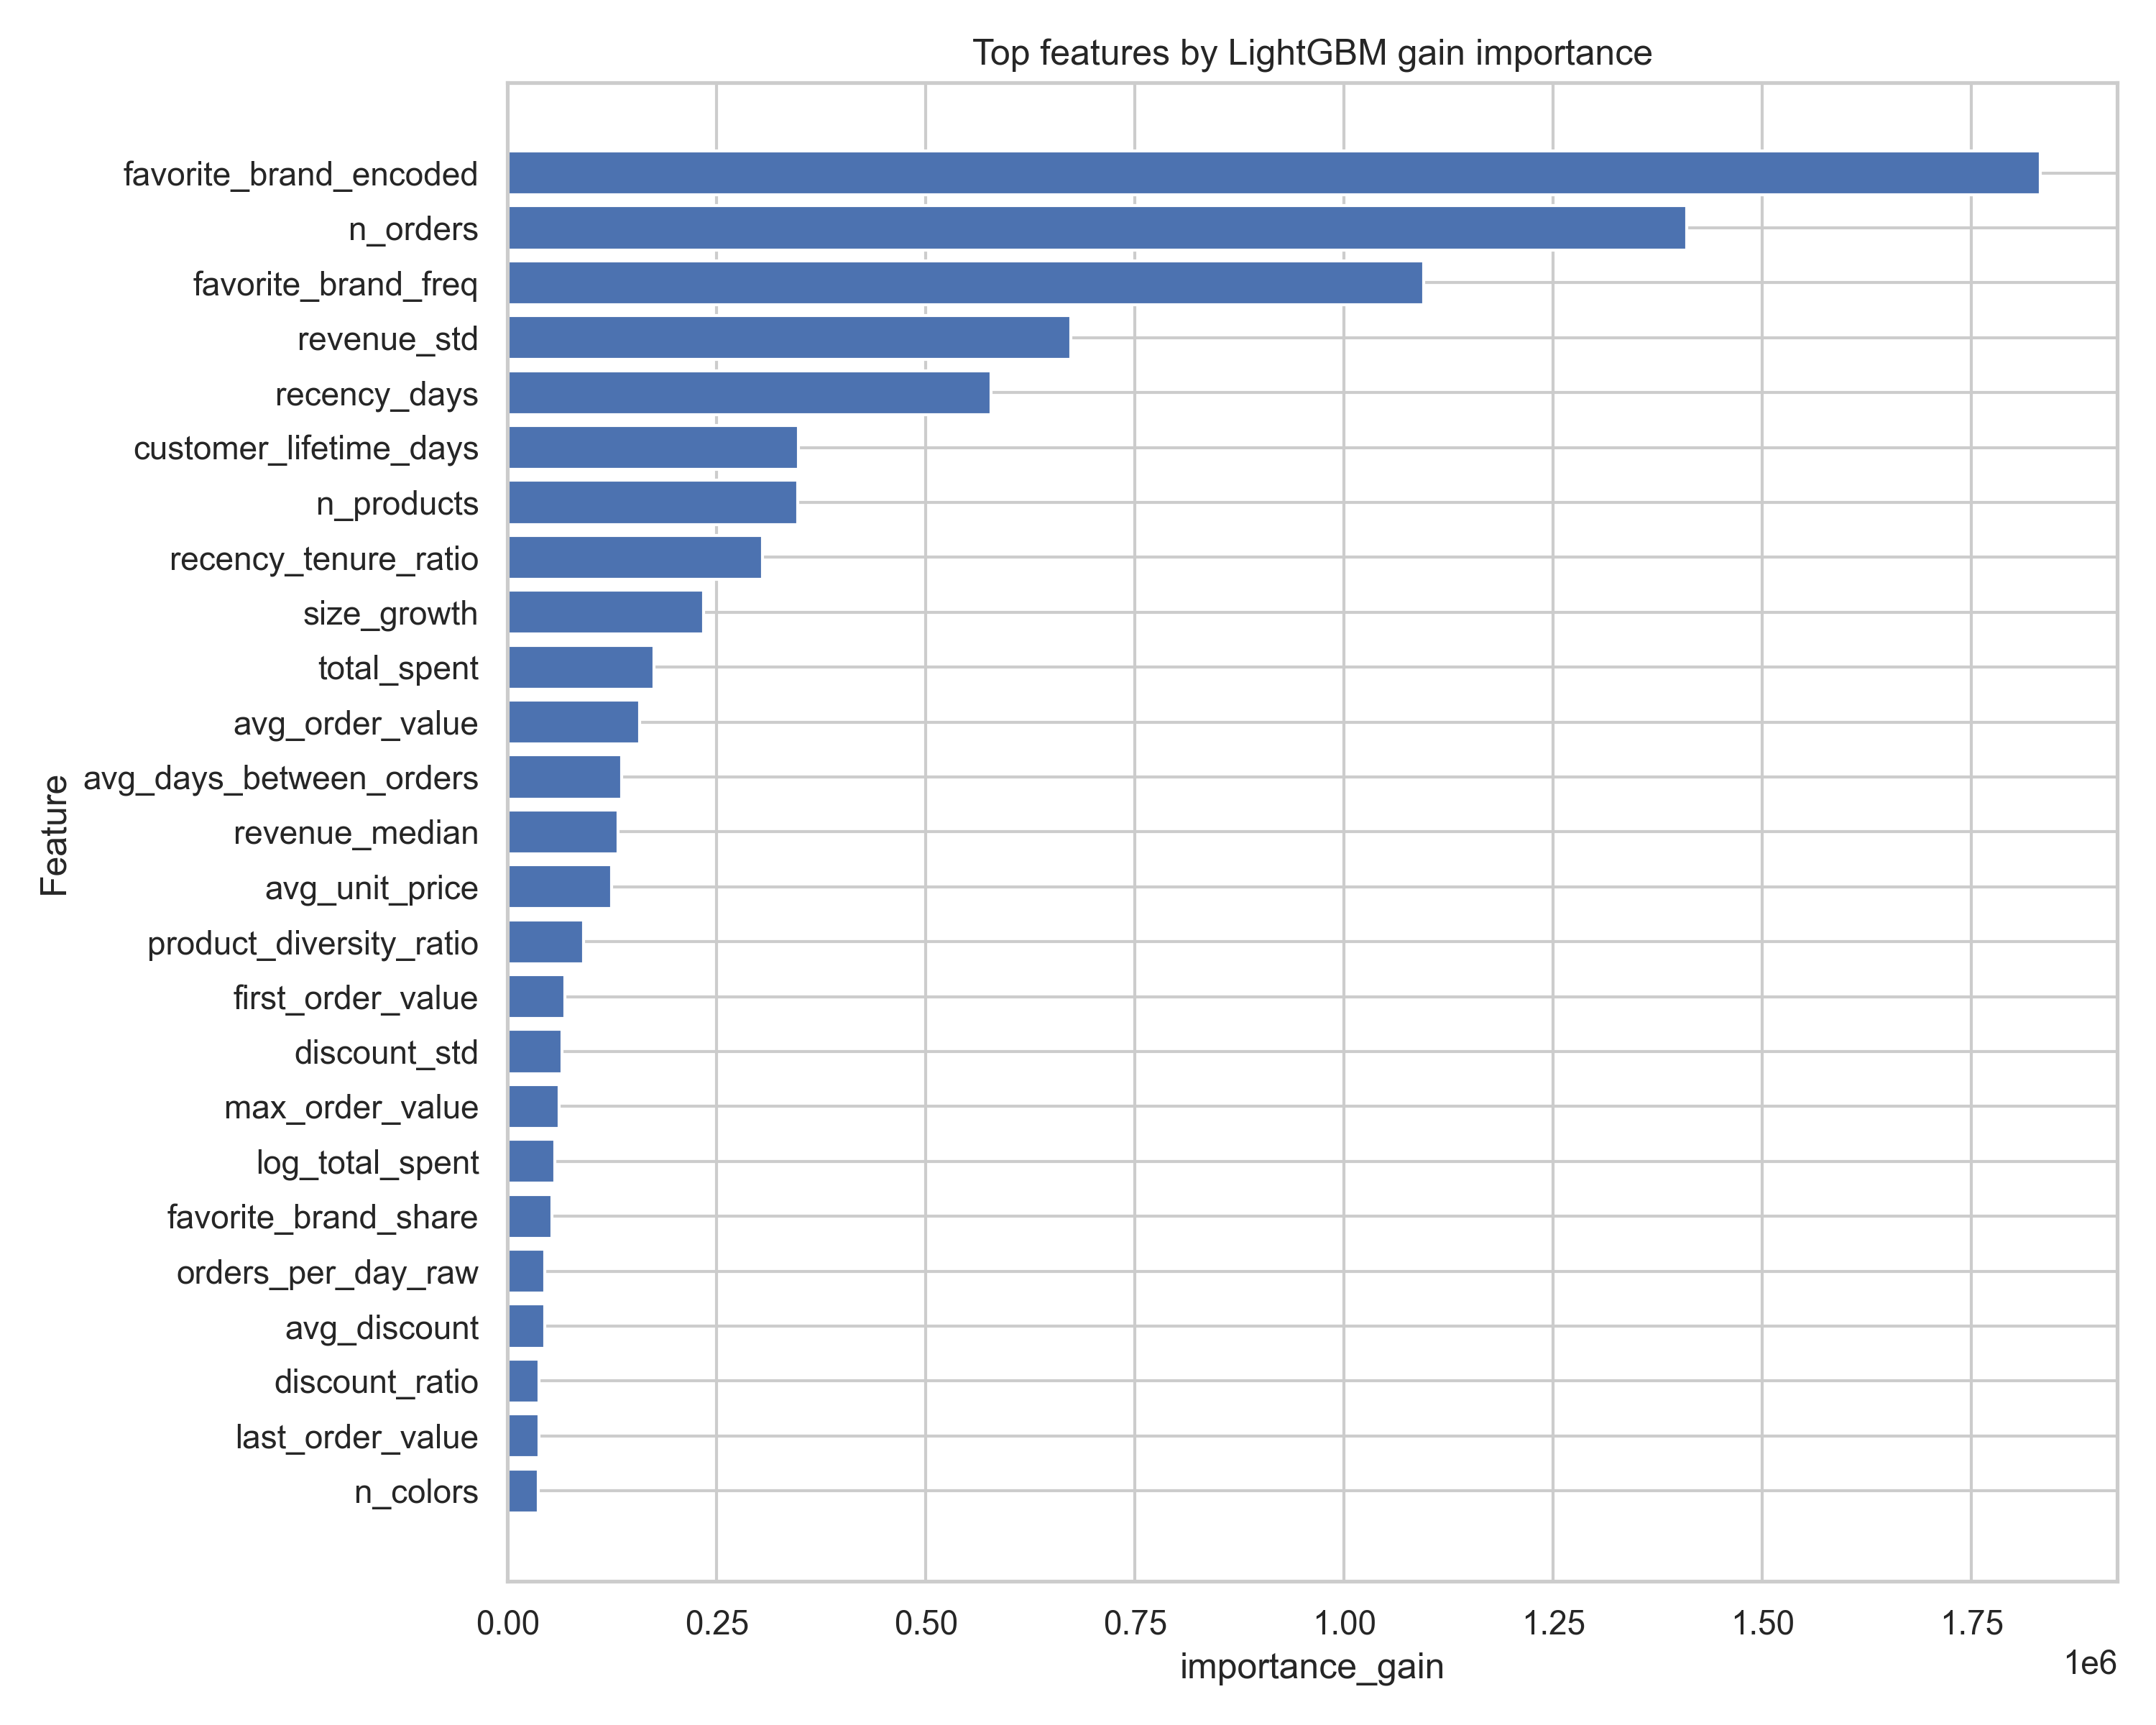
\includegraphics[width=\linewidth]{figures/14 feature_importance_gain.png}
\caption{LightGBM gain importance plot.}
\end{figure}

\subsection{Lightgbm split importance}
The split importance plot measures how frequently variables were used as splitting criteria throughout the decision trees. The variables favorite\_brand\_encoded, favorite\_brand\_freq, and recency\_days again appeared among the most frequently used. Unlike gain importance, split importance highlights variables that repeatedly partition the customer space, even where each split individually provides smaller improvements. The variables total\_spent, avg\_order\_value, and discount-related variables appeared much more frequently in the split importance ranking than in the gain importance ranking, suggesting that these variables contribute through many smaller non-linear interactions rather than through a few dominant decision boundaries.

\begin{figure}[H]
\centering
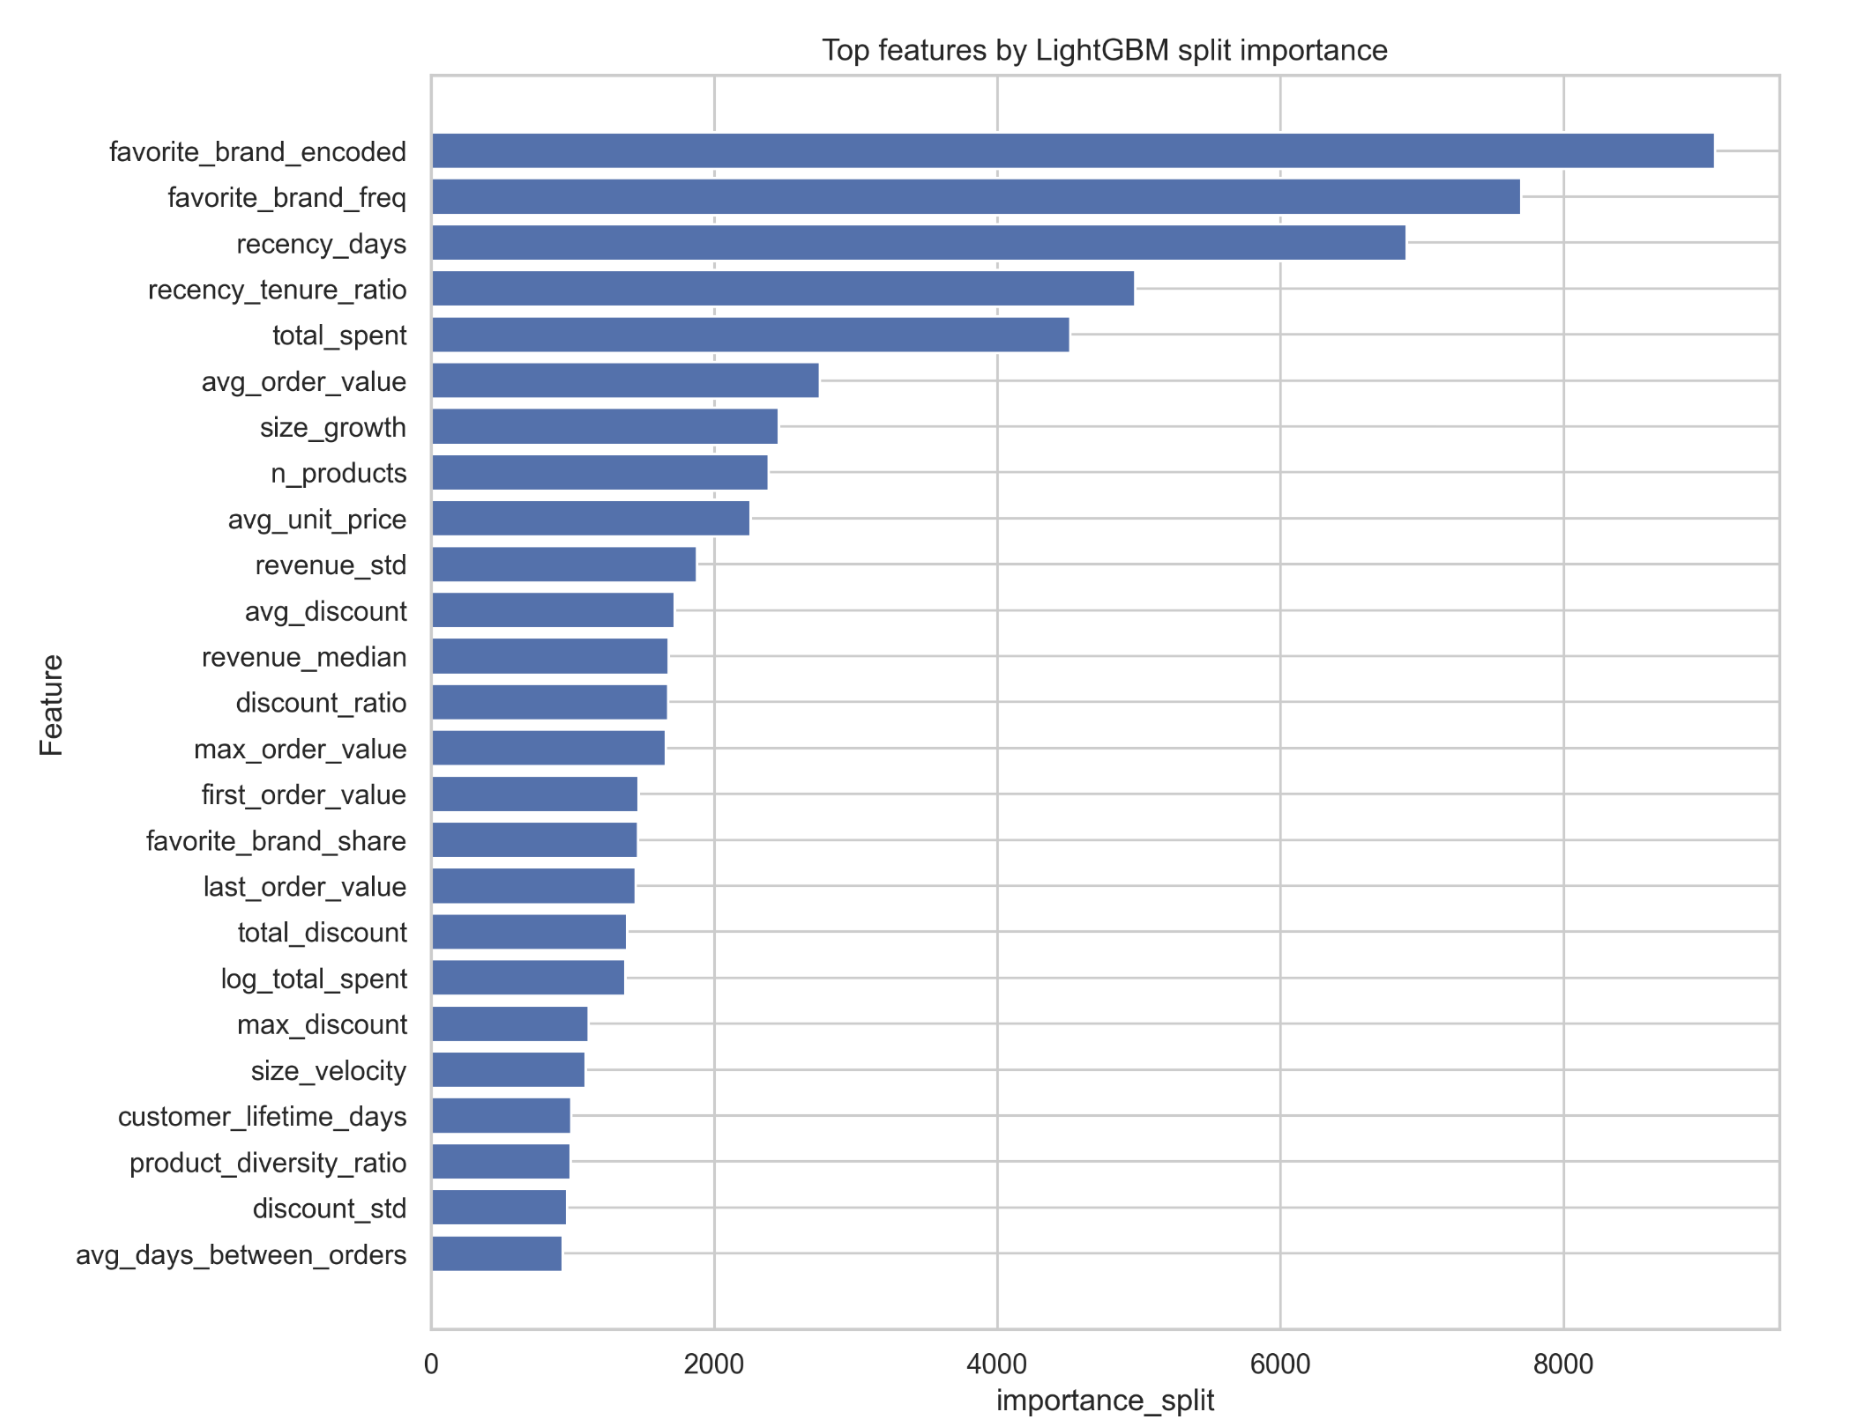
\includegraphics[width=\linewidth]{figures/15.png}
\caption{LightGBM split importance plot.}
\end{figure}

\subsection{Permutation importance}
Permutation importance was used as a more model-agnostic interpretation technique, measuring how strongly model performance deteriorated when each feature was randomly shuffled. The variable n\_orders was by far the most important, with a permutation importance score of 2.375, indicating that purchase frequency is the single most critical driver of predictive performance. Other highly influential variables included unique\_months, recency\_days, total\_spent, customer\_lifetime\_days, and recency\_tenure\_ratio. Notably, favorite\_brand\_encoded became substantially less dominant compared to the gain importance ranking, suggesting that part of its predictive contribution overlaps with other correlated behavioural variables. Permutation importance therefore provides a more conservative estimate of true standalone feature importance.

\begin{figure}[H]
\centering
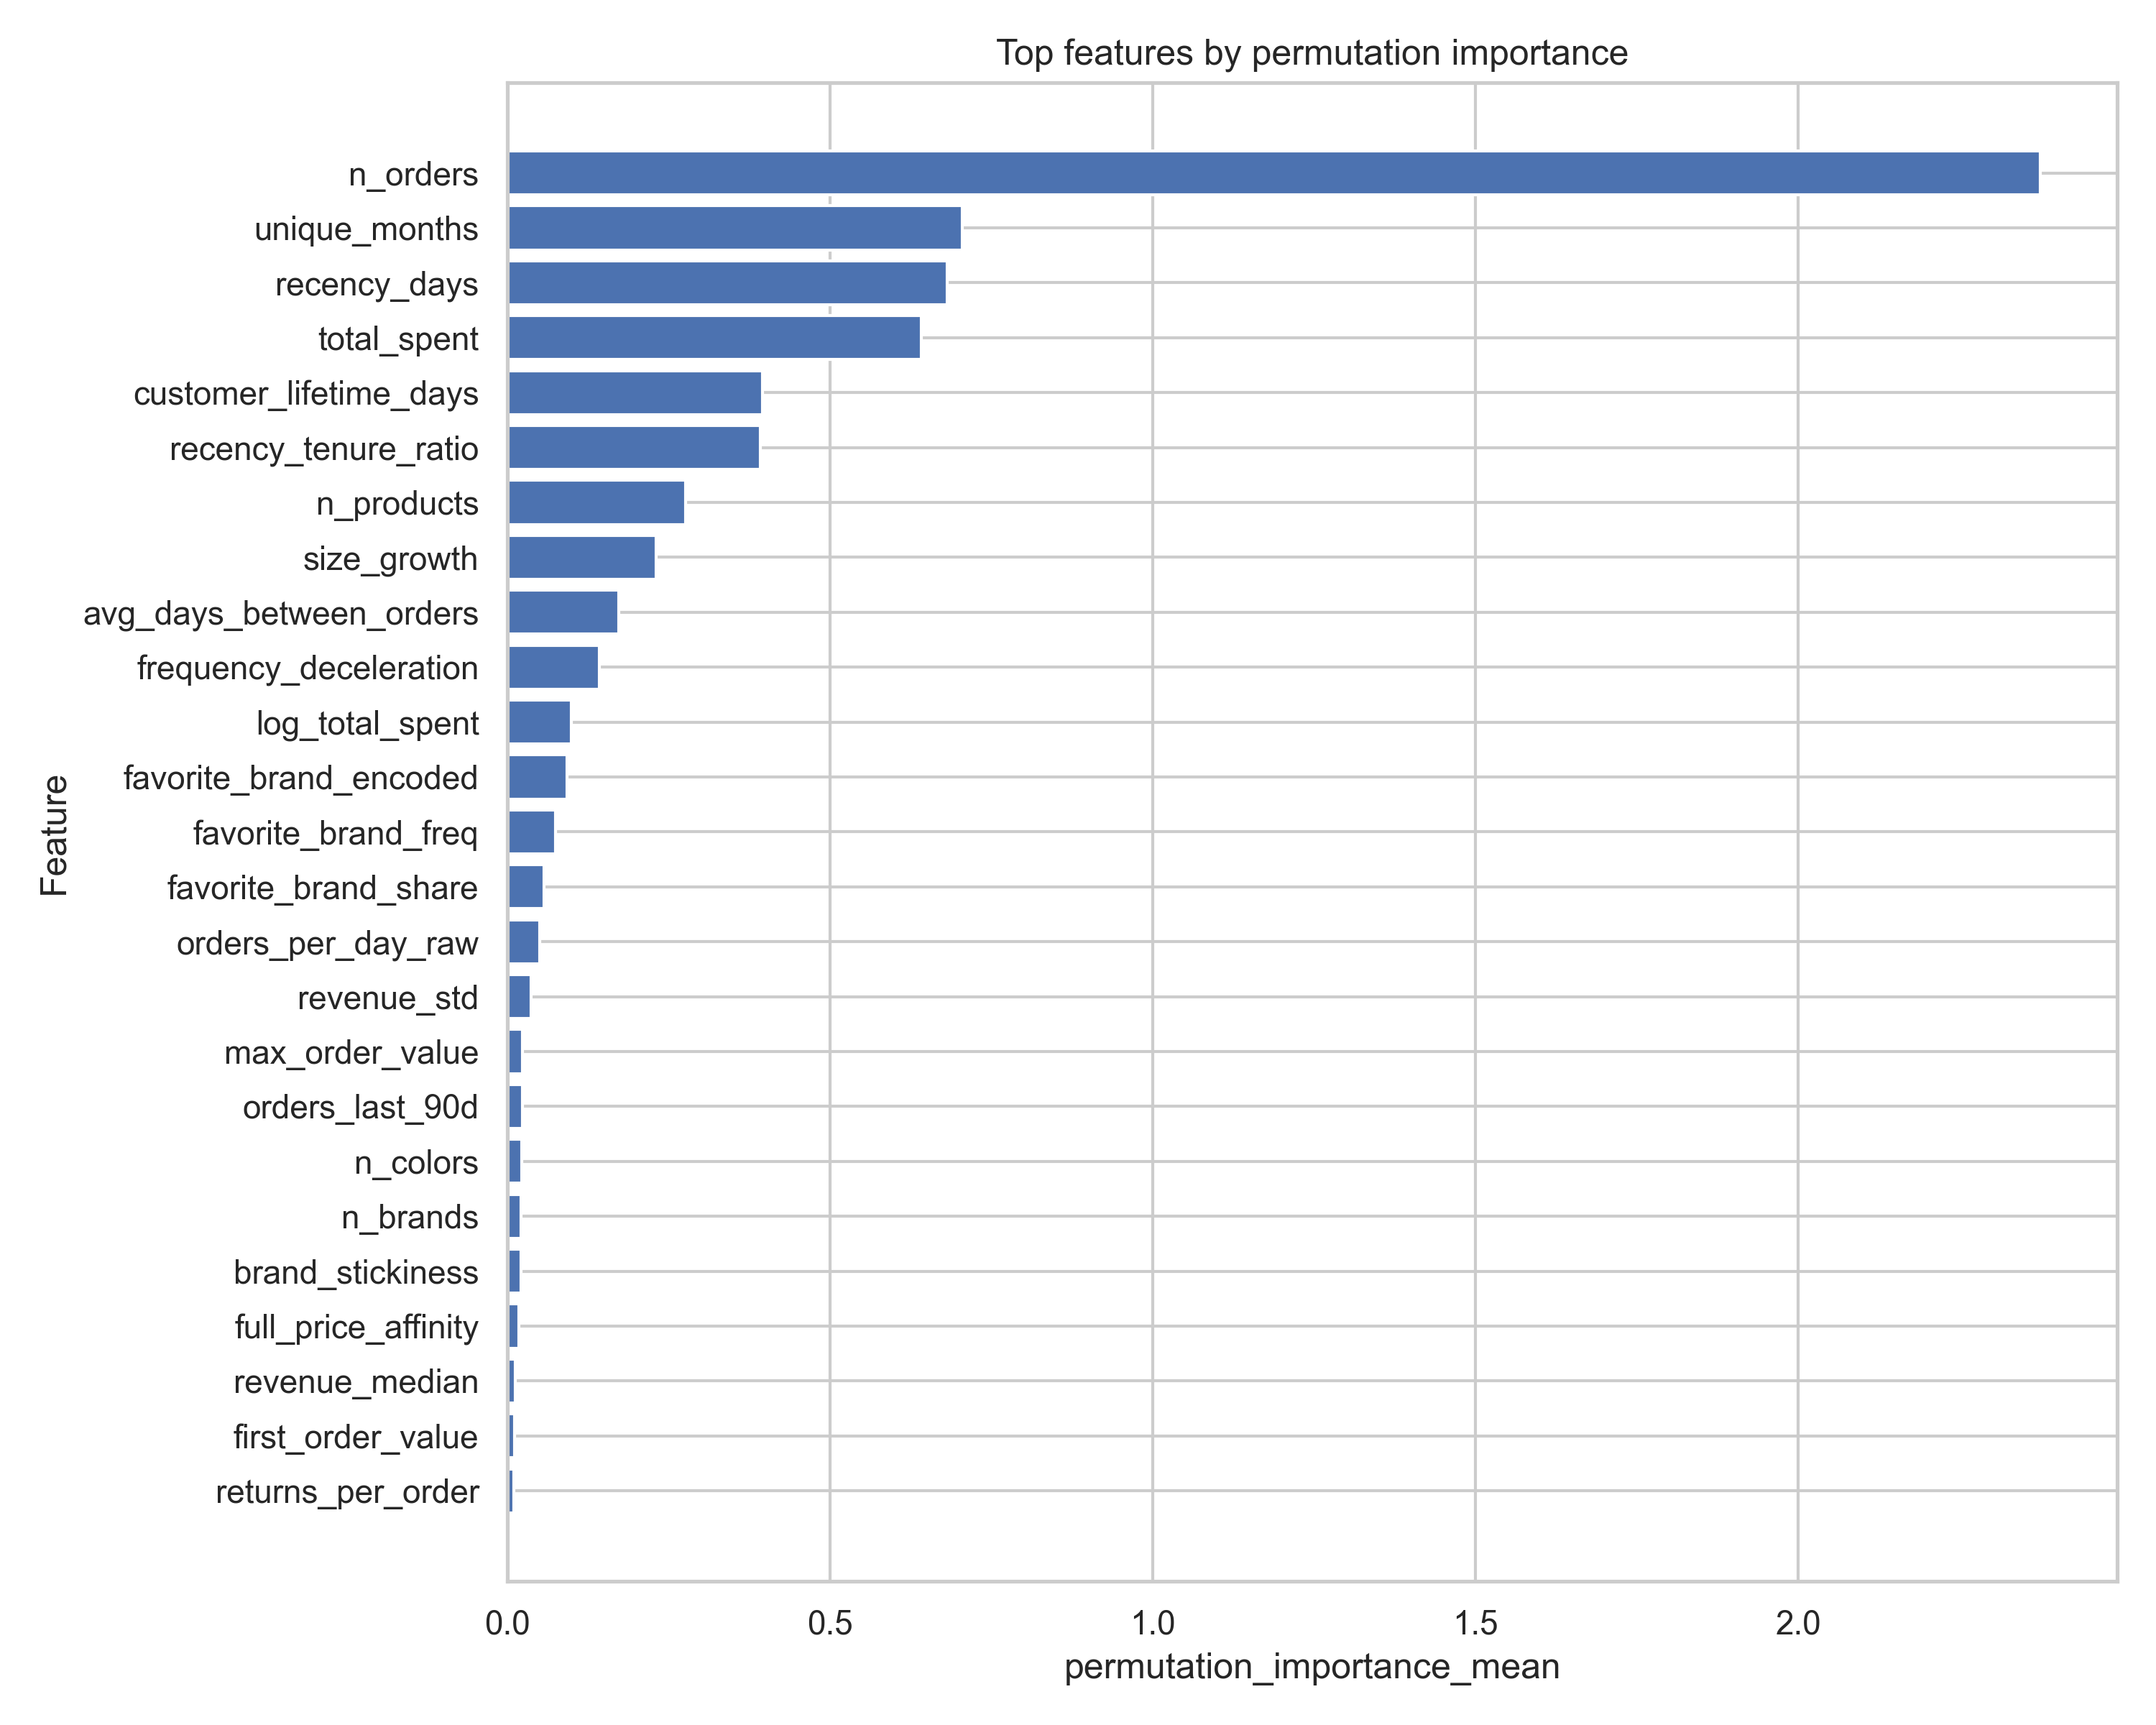
\includegraphics[width=\linewidth]{figures/16 feature_importance_permutation.png}
\caption{Permutation importance plot.}
\end{figure}

\subsection{Pca analysis}
PCA was used to study the global structure of the engineered customer feature space. The first principal component explained 27.73 percent of the total variance and the second explained 14.15 percent, together accounting for 41.88 percent of total variance. The first ten components together explained approximately 77.99 percent of total variance, indicating that the customer feature space has meaningful lower-dimensional structure despite the large number of engineered variables.

In the PCA visualisation, higher-revenue customers tended to appear more frequently toward larger positive PC1 values, though the separation remained only partially linear, confirming that non-linear modelling approaches remain necessary. The first principal component was mainly driven by n\_colors, n\_products, n\_brands, n\_orders, unique\_months, and customer\_lifetime\_days, all of which describe customer engagement intensity and behavioural diversity. Large positive PC1 values therefore characterised highly active long-term customers with broad purchasing behaviour. The variables total\_spent, log\_total\_spent, and orders\_per\_day also contributed strongly to PC1.

The second principal component was driven mainly by avg\_order\_value, revenue\_median, avg\_unit\_price, max\_order\_value, last\_order\_value, and recent\_revenue\_ratio, capturing spending intensity and transaction value rather than pure customer activity. Variables related to returns and discount behaviour also contributed moderately to PC2, suggesting that this component separates premium high-spending customers from more discount-sensitive or lower-value purchasing profiles.

\begin{figure}[H]
\centering
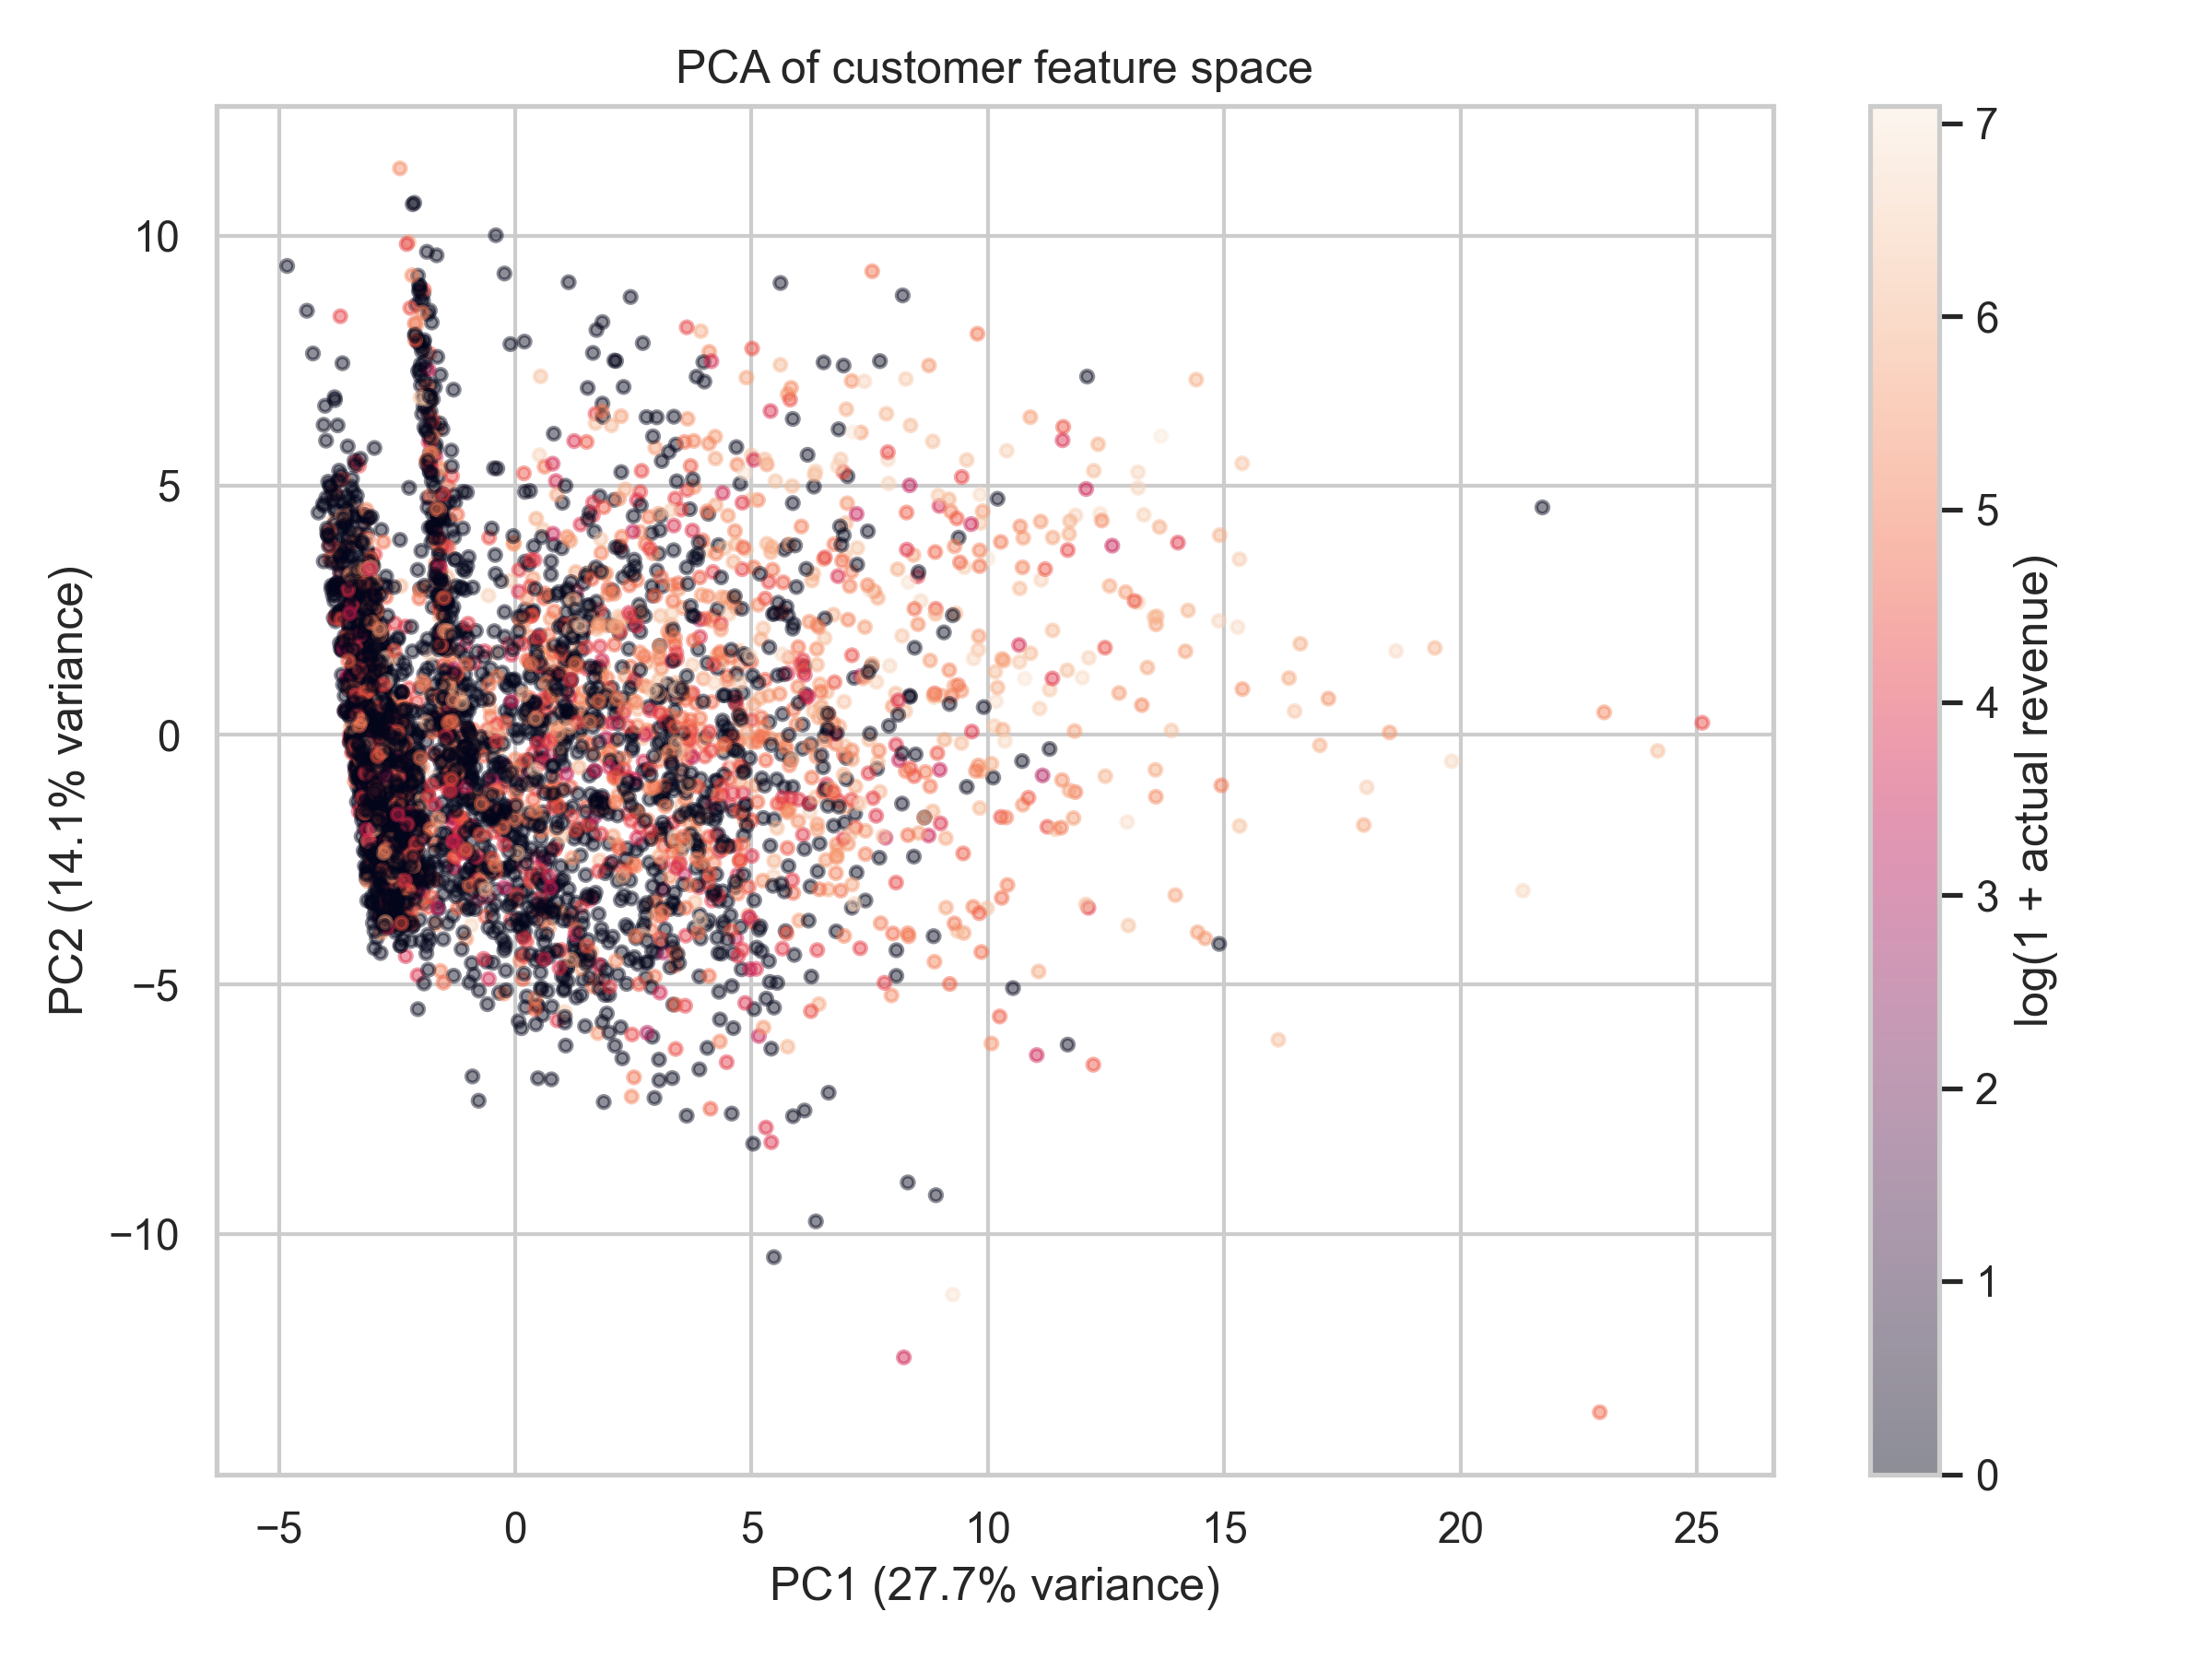
\includegraphics[width=\linewidth]{figures/17 pca_customer_feature_space.png}
\caption{PCA visualisation.}
\end{figure}
\begin{figure}[H]
    \centering
    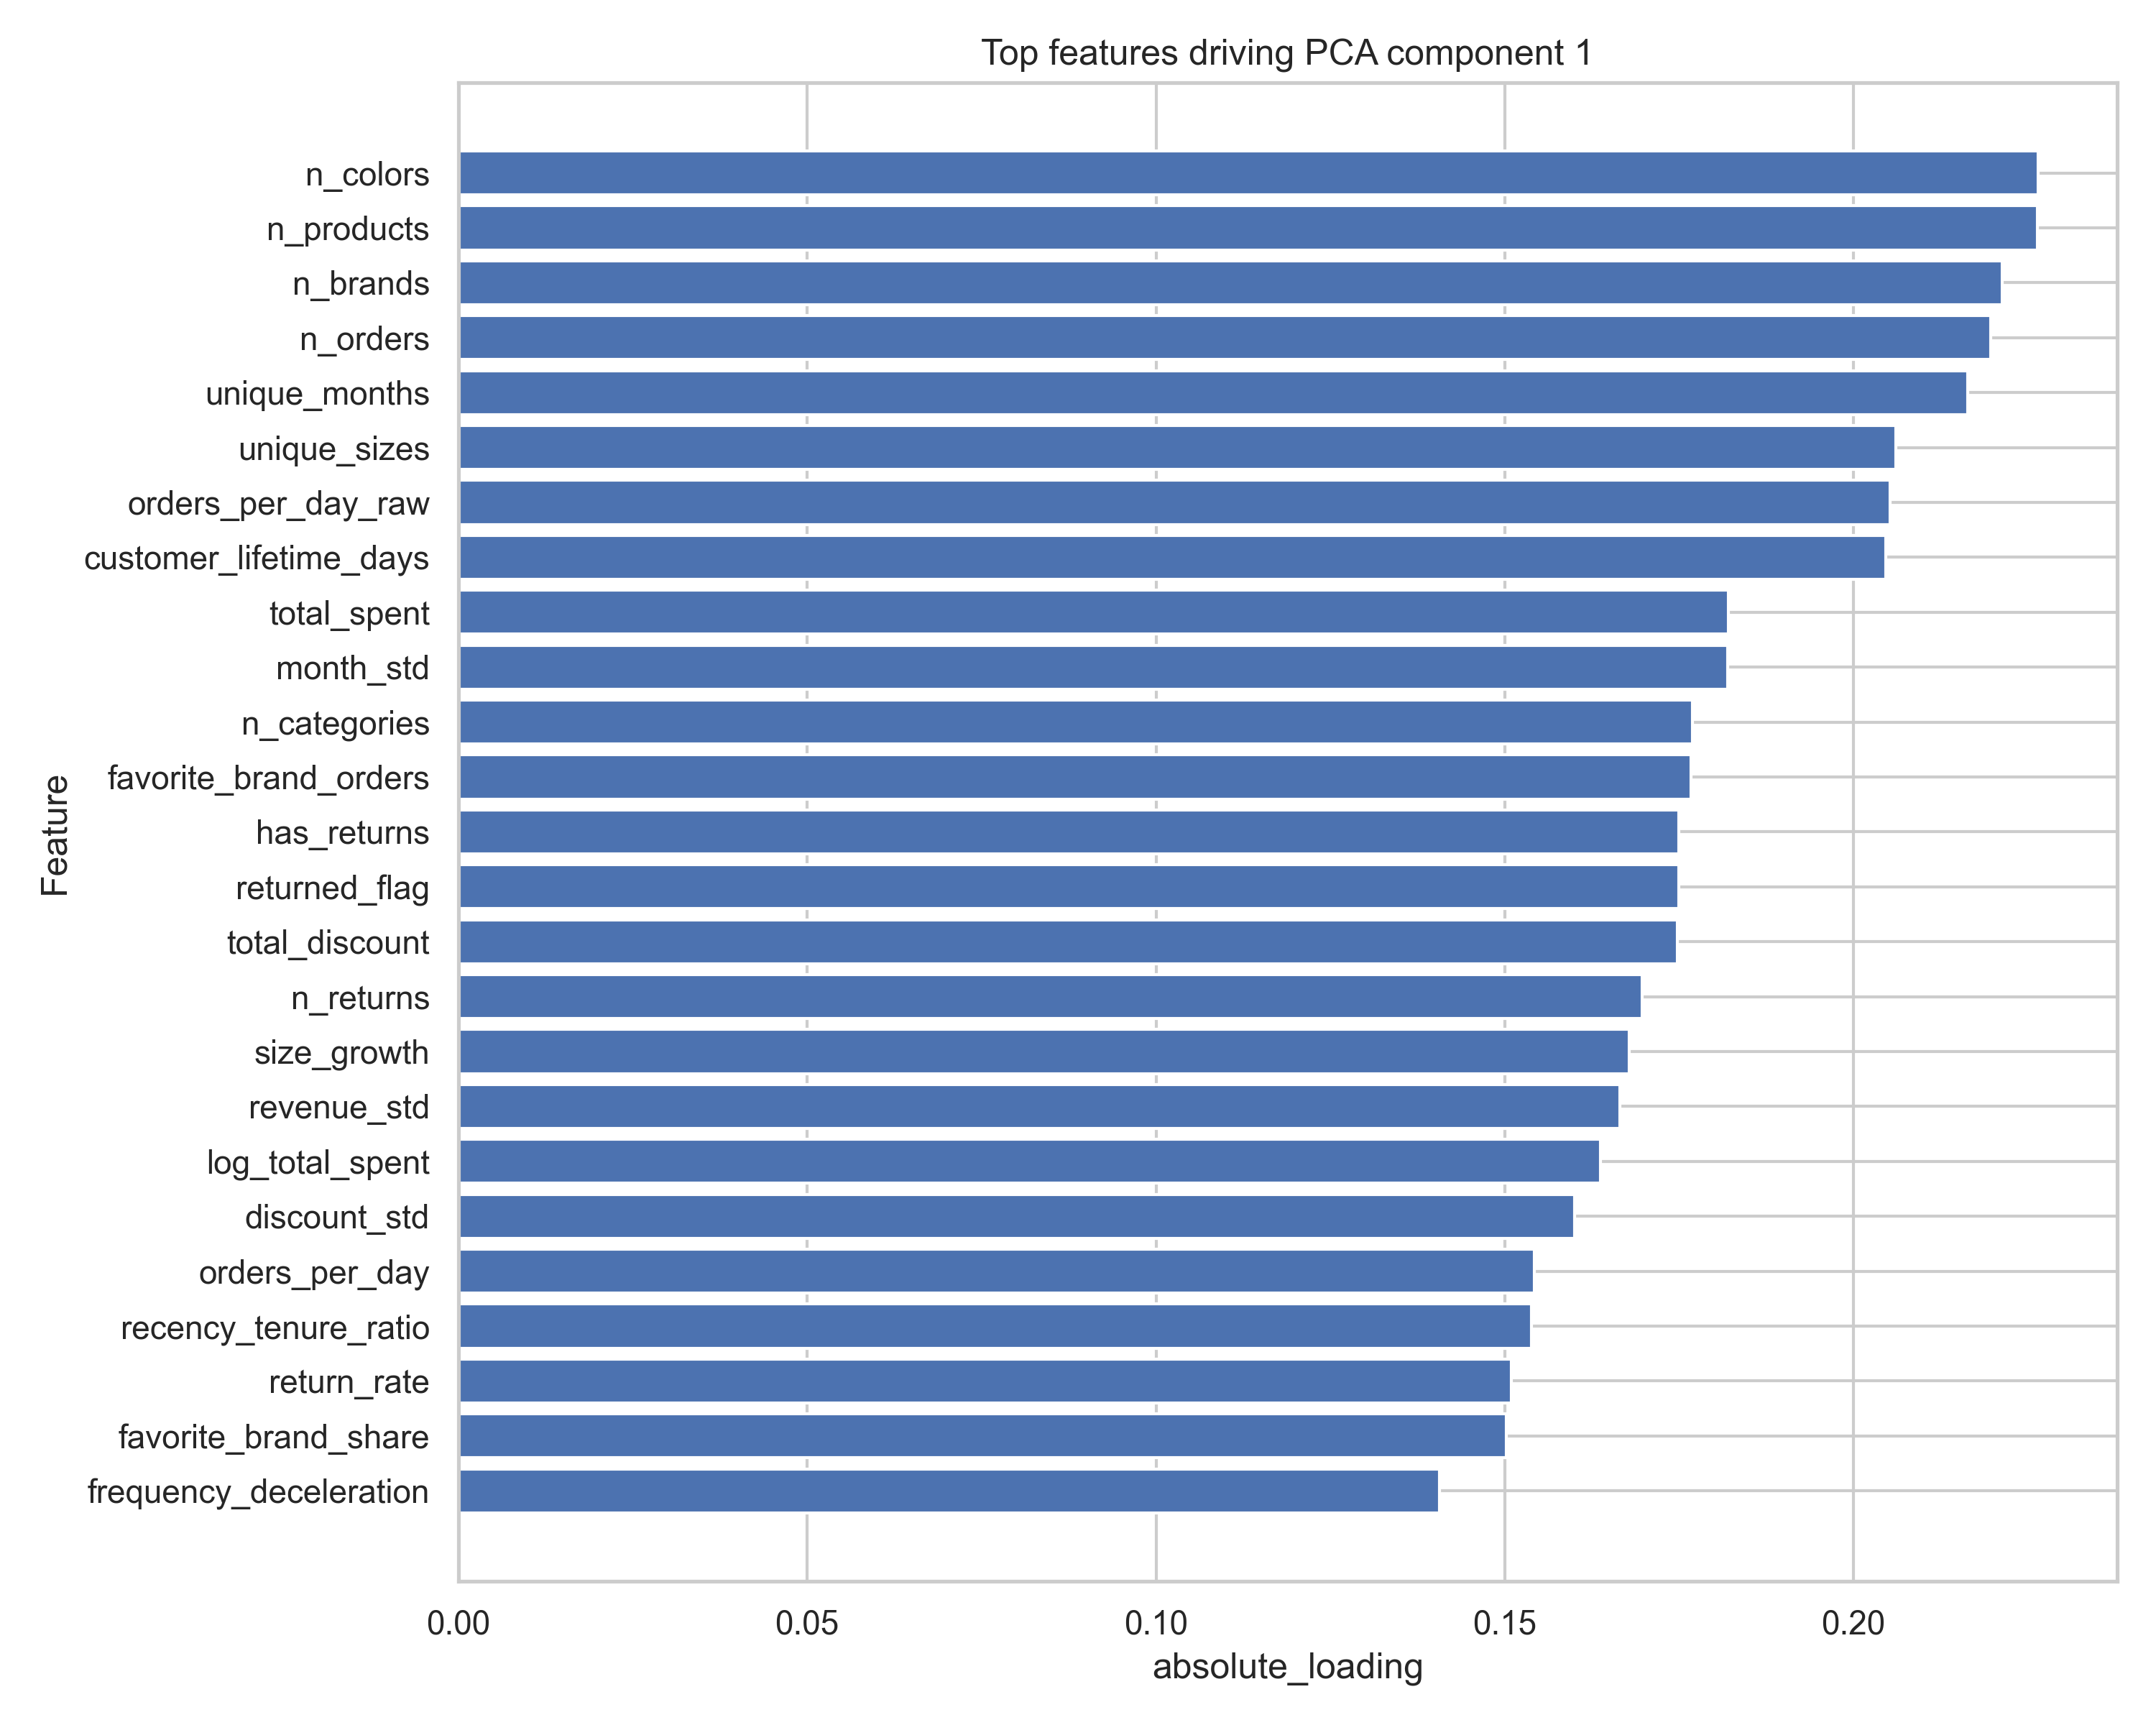
\includegraphics[width=0.7\textwidth]{figures/17.1 pca_pc1_top_loadings.png}
    \caption{PC1 top loadings.}
    \vspace{0.3cm}
    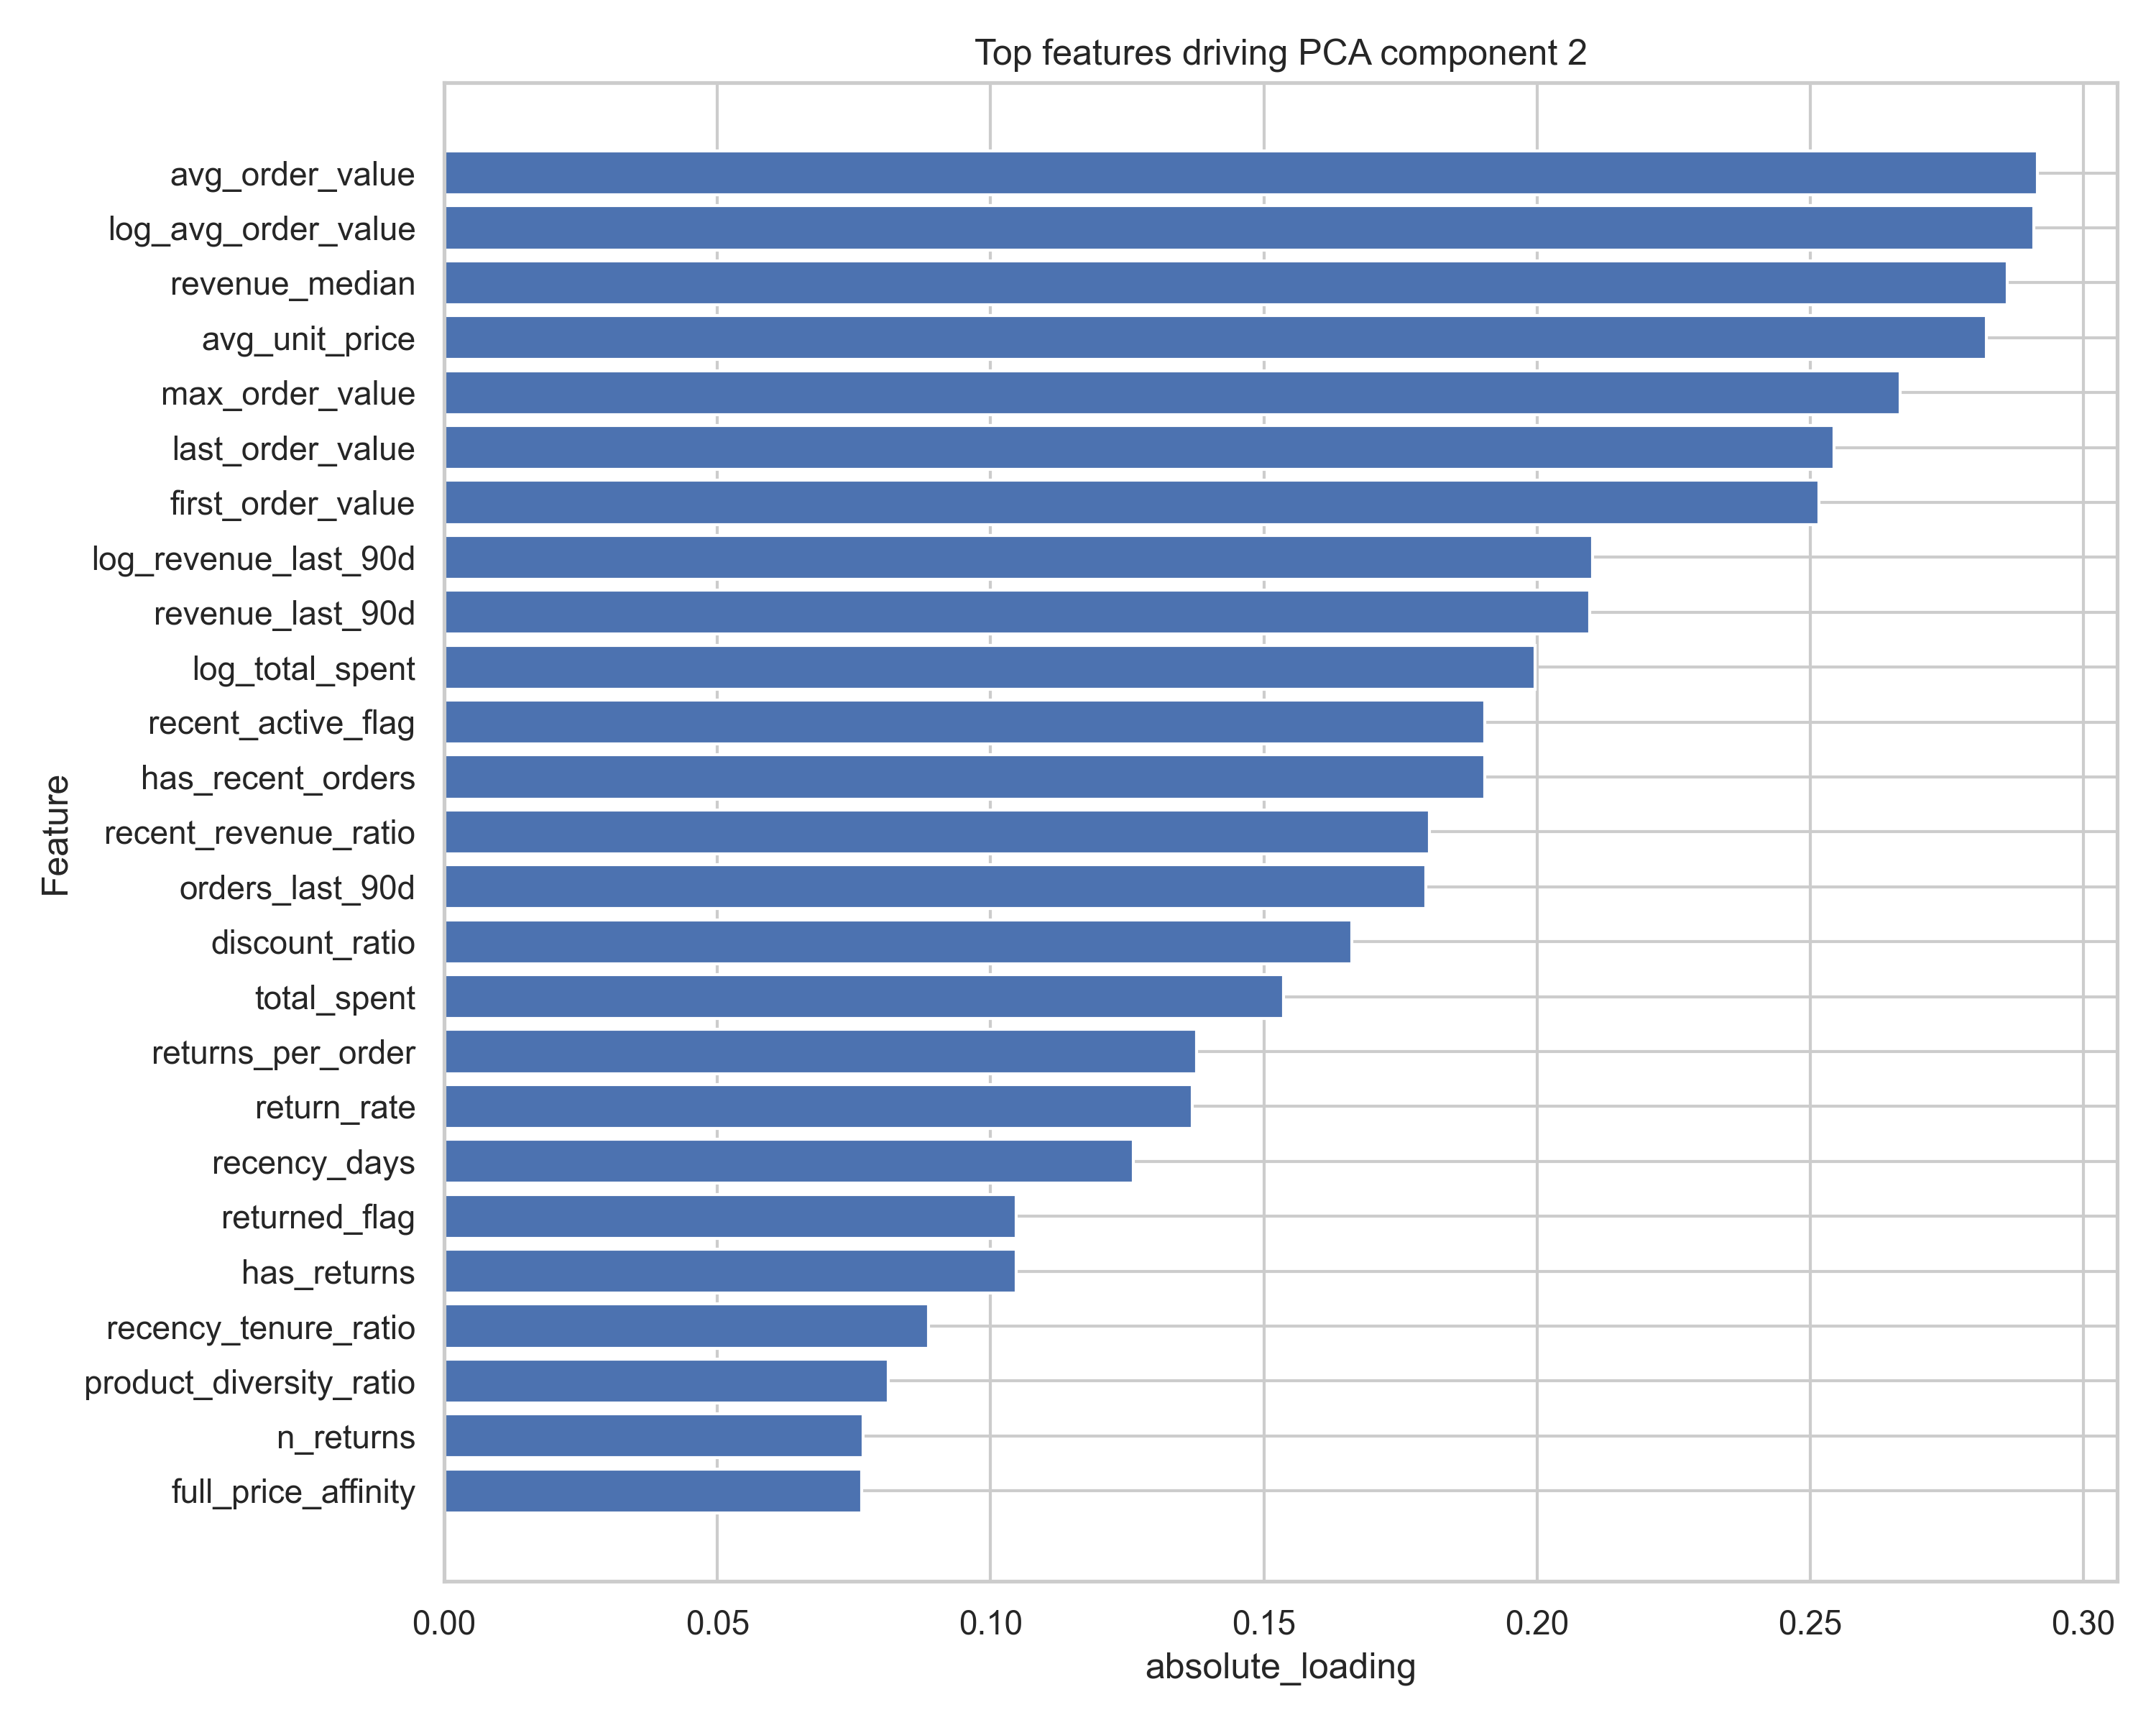
\includegraphics[width=0.7\textwidth]{figures/17.2 pca_pc2_top_loadings.png}
    \caption{PC2 top loadings.}
\end{figure}

\subsection{T-sne customer segmentation}
t-SNE was used as a non-linear dimensionality reduction technique to study local customer clustering structure. The axes of the t-SNE plot are not directly interpretable variables; rather, they are artificial coordinates produced by the algorithm to place customers with similar feature profiles close together. Customers positioned close together in the plot have similar historical behaviour, while those far apart are behaviourally more distinct.

The first t-SNE plot coloured customers by log-transformed future revenue revealed several distinct clusters, but high-revenue and zero-revenue customers still overlapped substantially, confirming that future revenue is difficult to predict perfectly even in the behavioural feature space. To interpret the clusters further, the same t-SNE coordinates were coloured by individual model features. The variable customer\_lifetime\_days showed a clear pattern, with long-lifetime customers concentrated in specific clusters in the central-right part of the map. The variables recency\_days and recency\_tenure\_ratio also showed strong structure, indicating that inactive customers occupied different regions from recently active ones. The variables n\_orders and total\_spent highlighted smaller groups of highly active or high-value customers, while unique\_months and revenue\_std varied across clusters, suggesting that seasonality and spending volatility help distinguish customer types. The variable favorite\_brand\_freq showed that some clusters were partly related to brand-popularity patterns, though this structure was less directly linked to future revenue than activity and recency features.

Overall, the t-SNE analysis indicated that the engineered features capture meaningful behavioural segments mainly driven by activity level, recency, customer lifetime, spending scale, and brand preference. However, because revenue values still overlapped within many clusters, these segments were informative but not perfectly separable.

\begin{figure}[H]
    \centering
    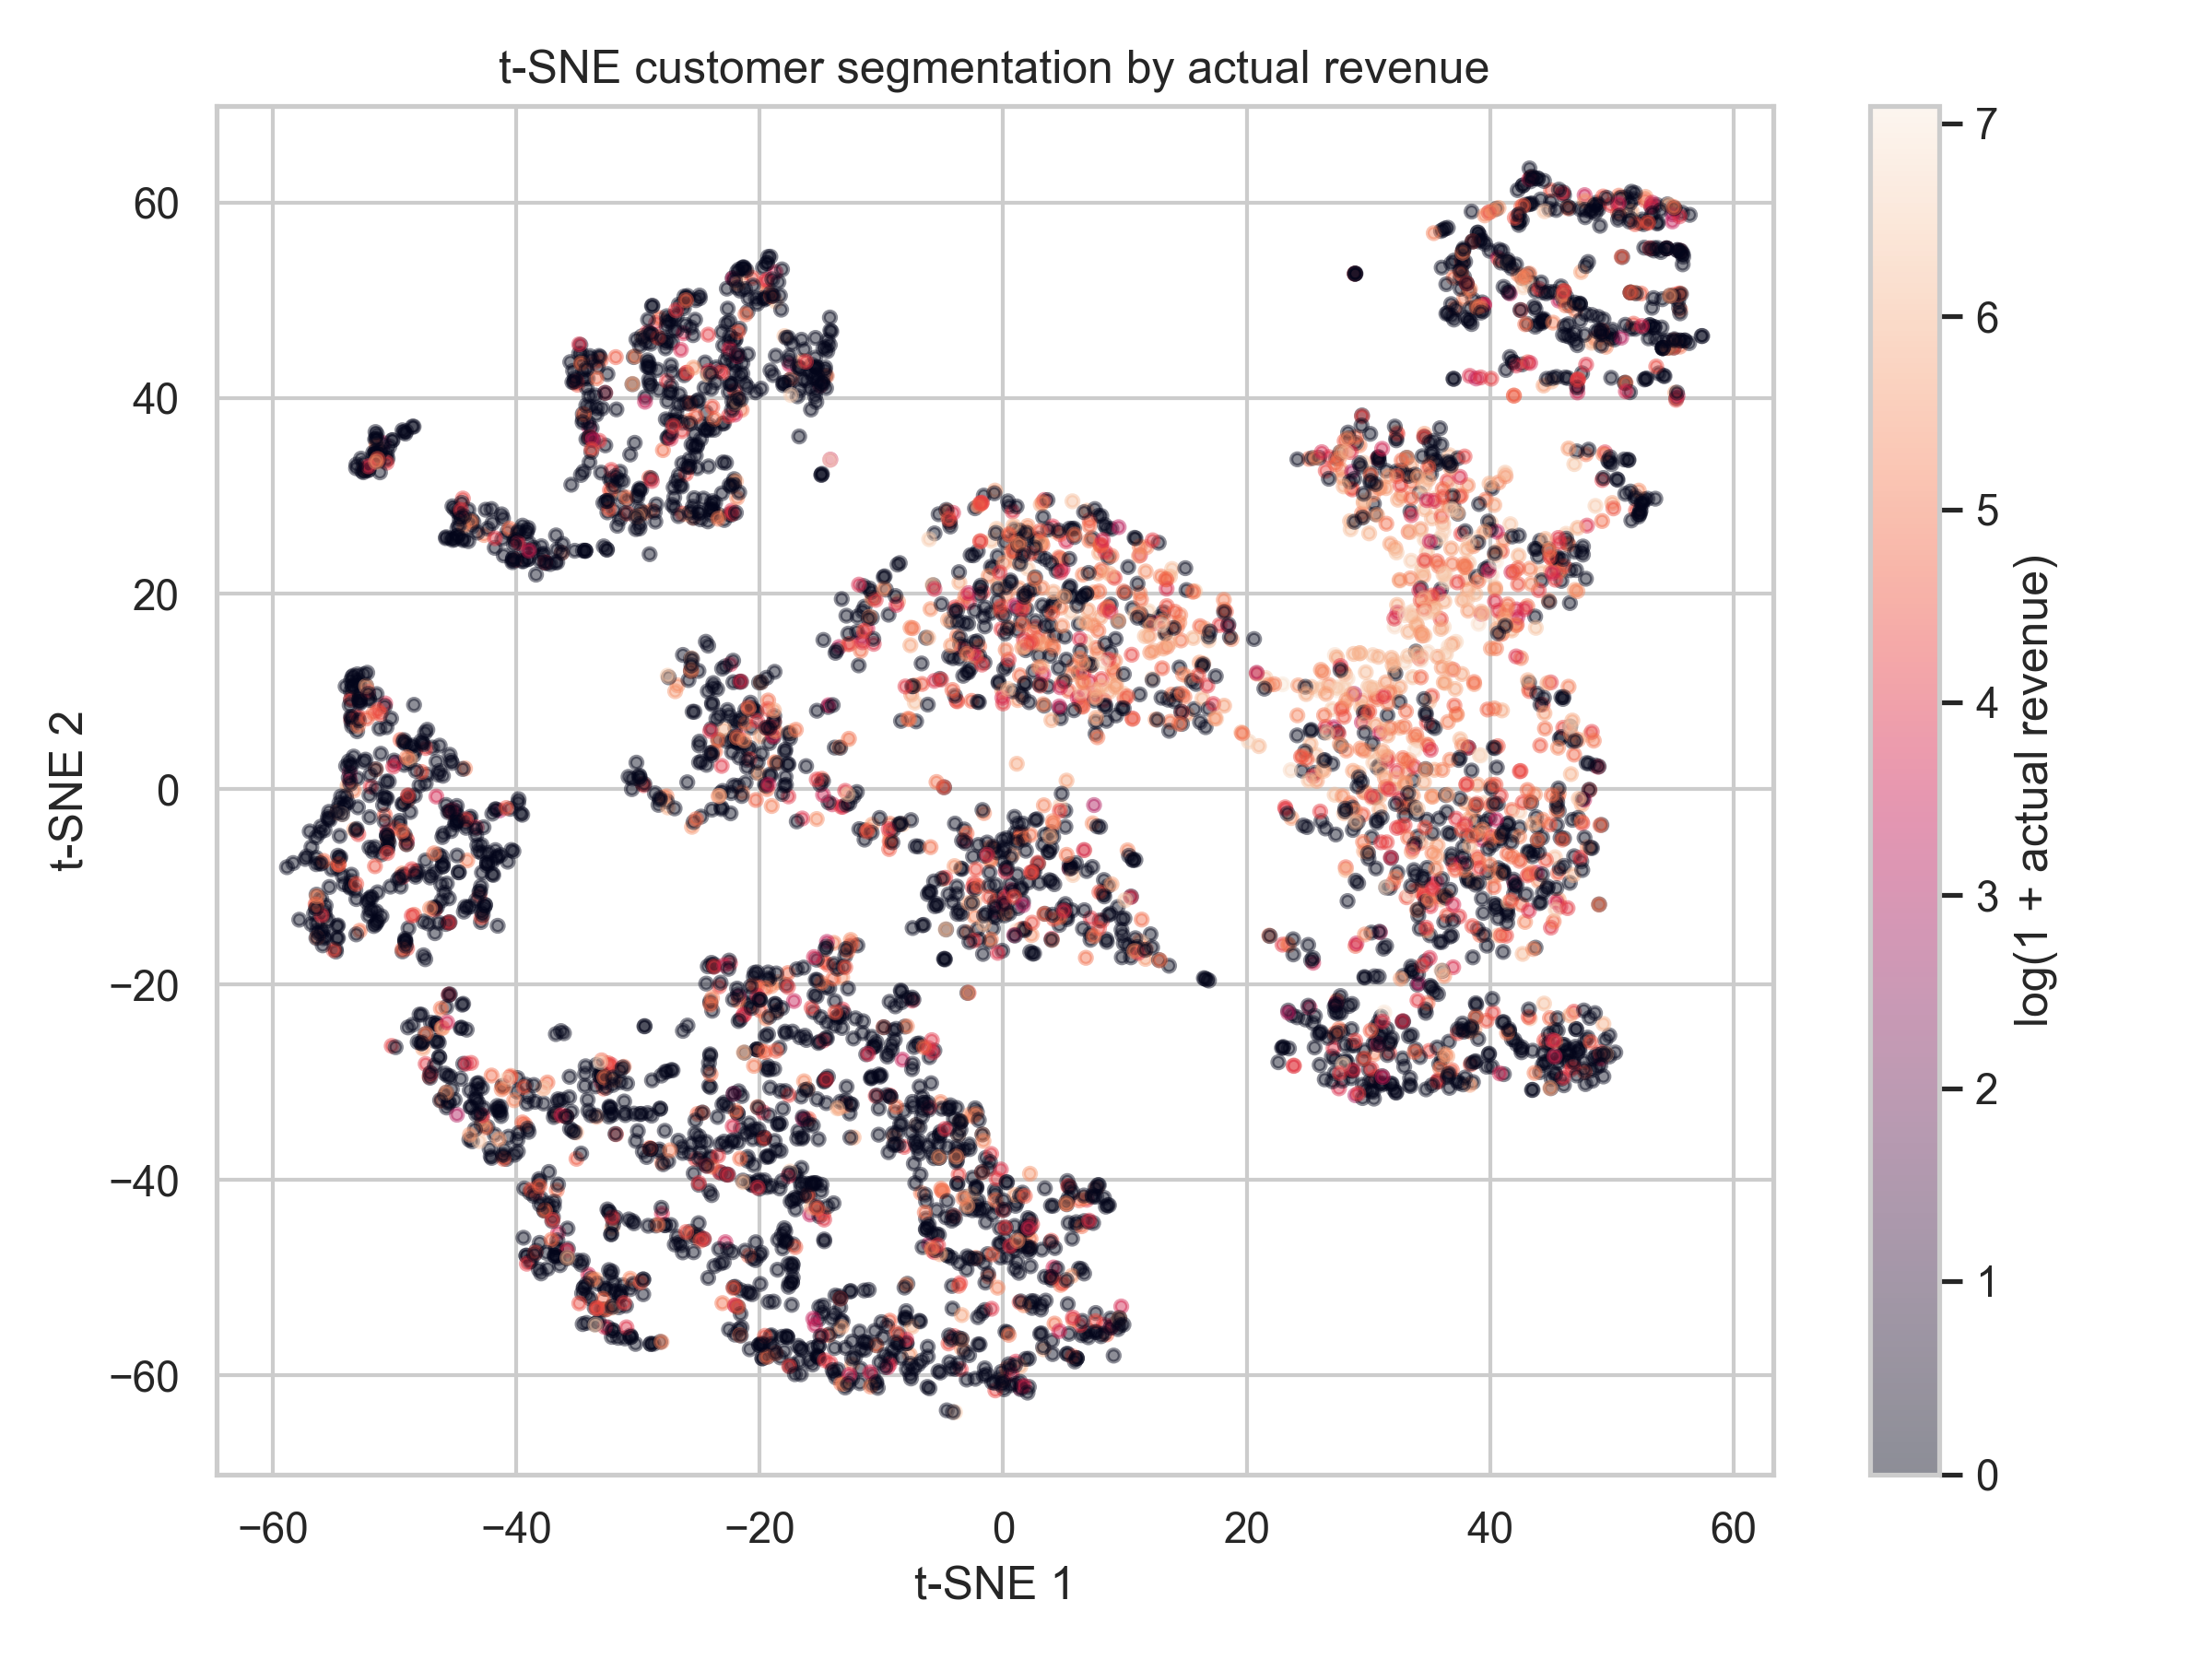
\includegraphics[width=0.9\textwidth]{figures/18 tsne_customer_segments.png}
    \caption{t-SNE customer segmentation.}
\end{figure}

\begin{figure}[H]
    \centering
    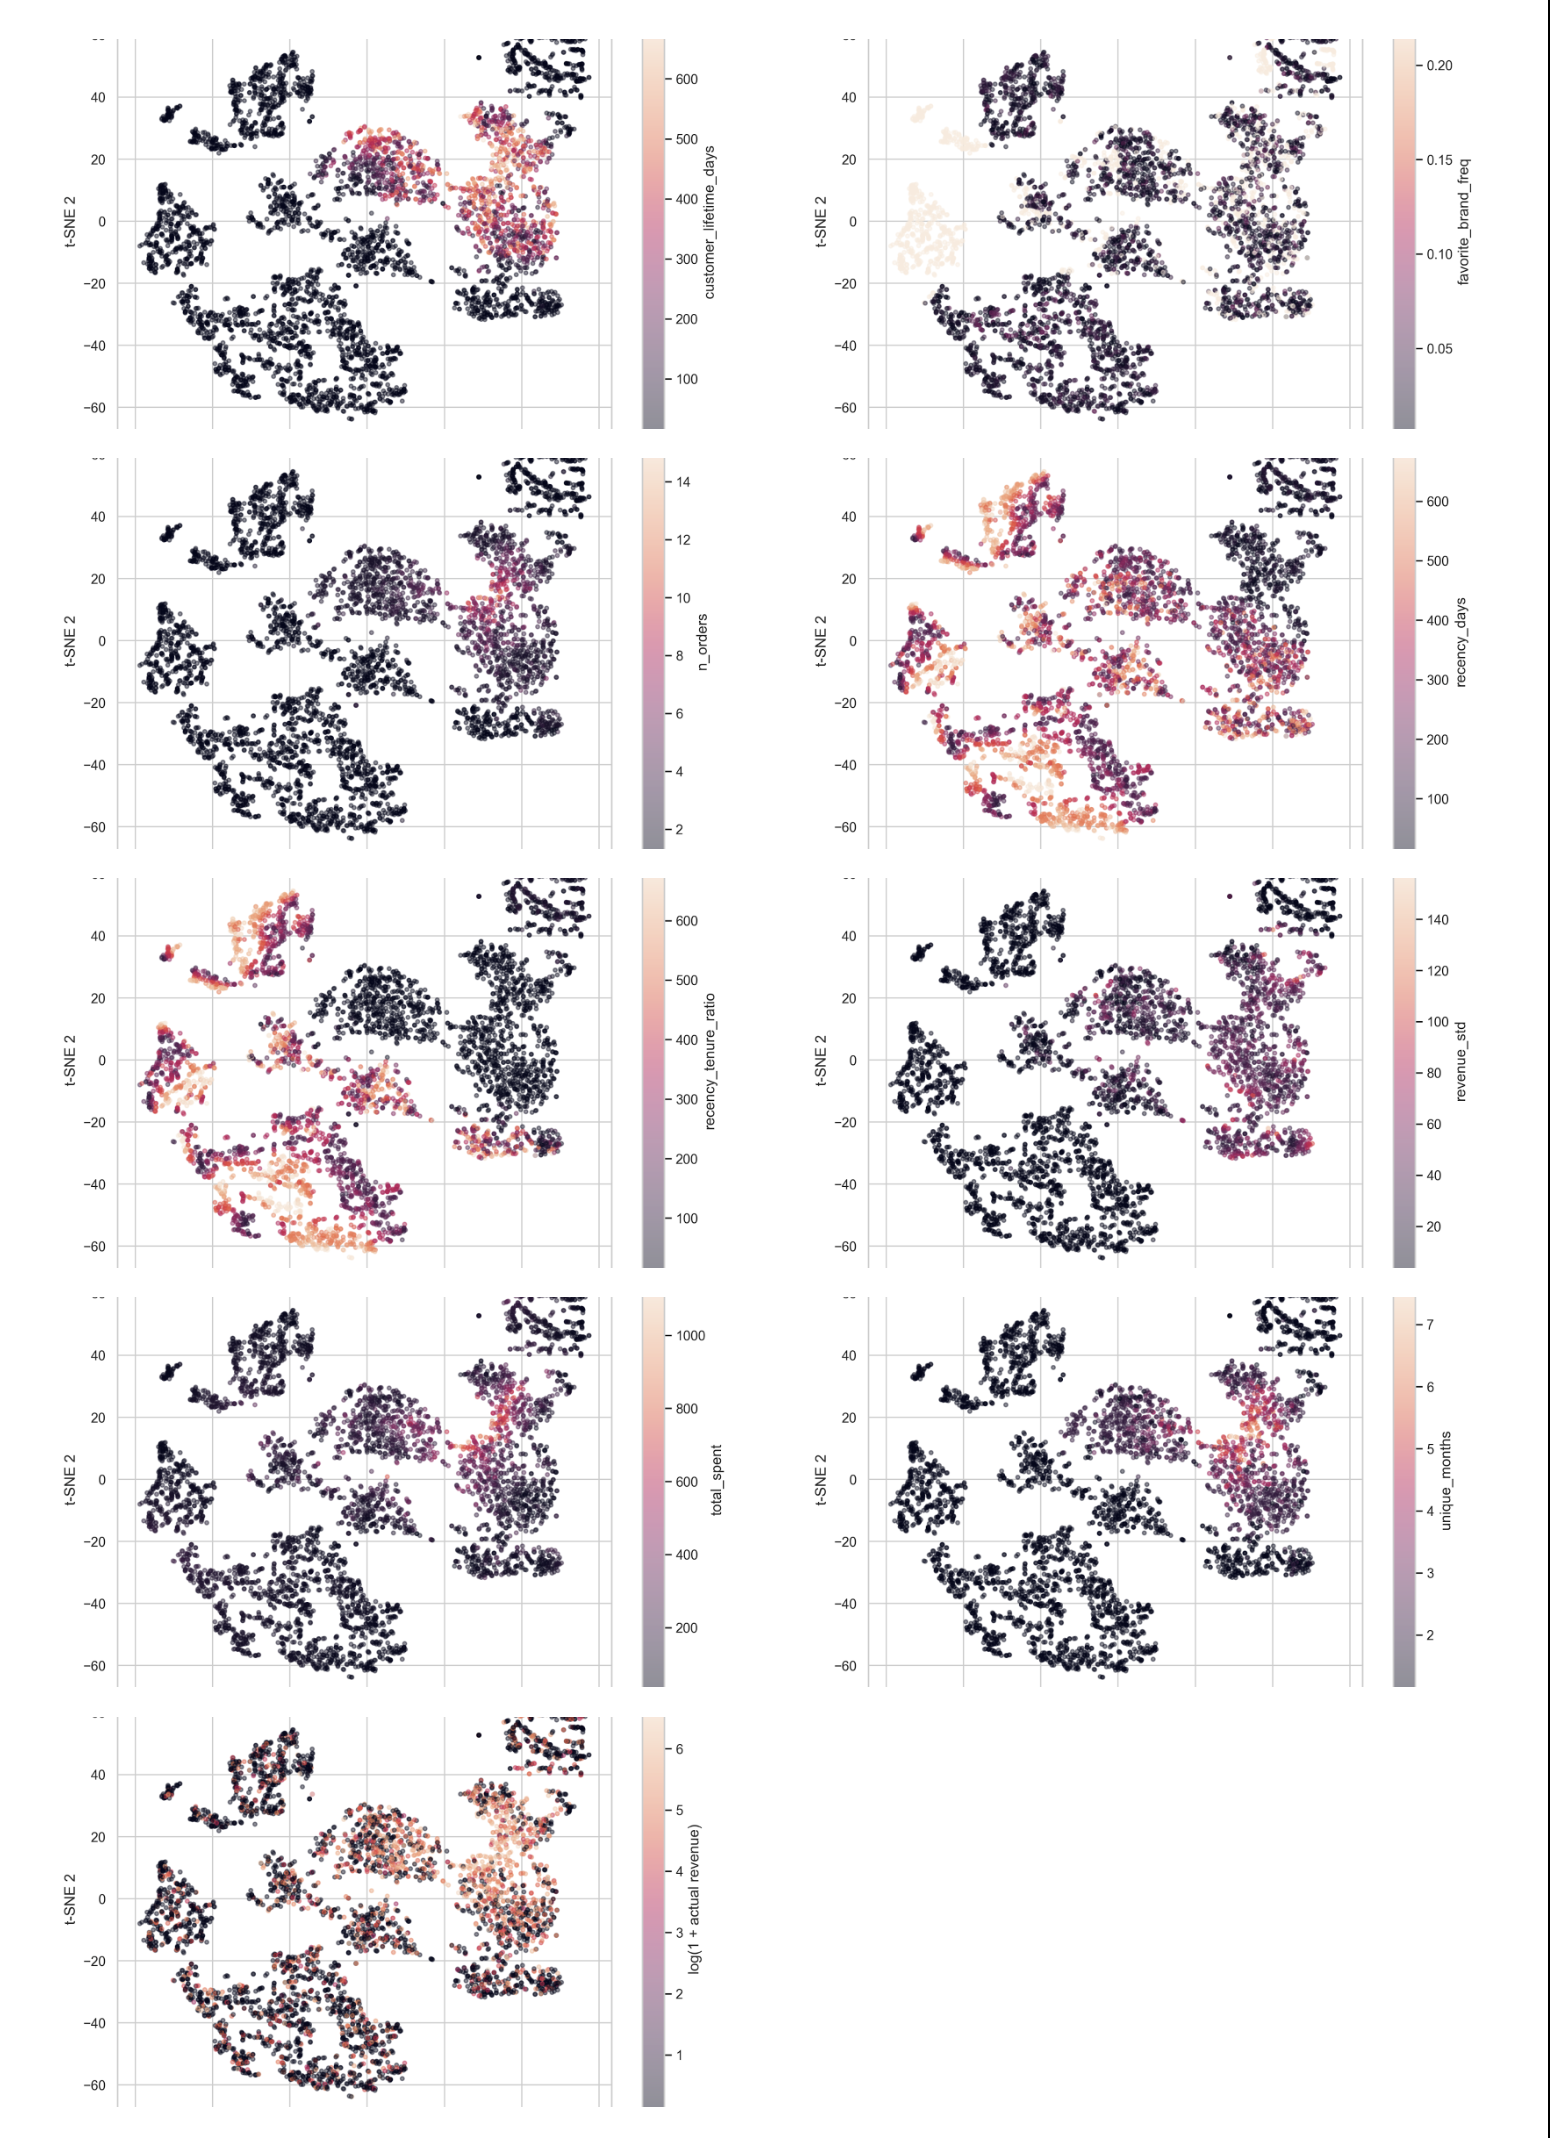
\includegraphics[width=0.9\textwidth]{figures/18.1 tsne_all.png}
    \caption{t-SNE components.}
\end{figure}

\subsection{Conclusion and business insights}
The interpretation analysis provides several business insights for customer relationship management and revenue optimisation. Recency consistently emerged as one of the strongest predictive variables, suggesting that recently active customers should be prioritised in retention and remarketing campaigns. Purchase frequency and long-term activity were also highly important, indicating that repeat customers generate more predictable future revenue than occasional buyers.
Customers with broad purchasing behaviour across multiple brands, products and shopping periods tended to have higher predicted future value. This suggests that behavioural diversity is an indicator of long-term engagement and loyalty. Brand-related variables were among the strongest model features, implying that brand preference contains valuable behavioural information beyond spending history and that some brands may attract more loyal or higher-value segments.
The importance of spending variability and transaction intensity shows that the model captures not only how much customers spend, but also how consistently and actively they interact with the retailer. PCA and t-SNE revealed meaningful segmentation structure, with groups such as highly active loyal customers, recently inactive customers, discount-sensitive customers and premium high-spending customers. These findings can support targeted marketing, loyalty programmes and retention campaigns. Overall, future customer revenue is driven mainly by long-term engagement, recent activity, behavioural consistency and loyalty patterns rather than isolated high-value purchases.


\section{Results and leaderboard performance}
\subsection{Submission results}
The final submission achieved a public leaderboard MAE of 61.537 and a Spearman correlation of 0.419. Following the reveal of the hidden leaderboard, the final results were as follows: a hidden leaderboard MAE of 62.628 (compared to a public score of 61.537), a secondary hidden score (Spearman correlation) of 0.405 (compared to a public score of 0.419), and a total of 123 submissions.

\begin{table}[H]
    \centering
    \begin{tabular}{l c c c c}
        \toprule
        Score & Public Score & Secondary score & Secondary Public Score & Entries \\
        \midrule
        62.628 & 61.537 & 0.405 & 0.419 & 123 \\
        \bottomrule
    \end{tabular}
    \caption{Final leaderboard submission results.}
    \label{tab:leaderboard_results}
\end{table}



\subsection{Analysis}
The transition from the public leaderboard to the hidden leaderboard provided important diagnostics about model behaviour under blind conditions. The primary MAE increased from 61.537 on the public split to 62.628 on the hidden split, indicating a minor generalisation gap. Because the hidden test set is an independent market slice, it may have contained a slightly higher concentration of volatile high-value buyers or unpredictable spending magnitudes, which naturally increased the L1 error.
Major data leakage is unlikely because the public-to-hidden difference was controlled and relatively small. If substantial leakage had occurred, the public score would probably have been unrealistically strong and the hidden deterioration much larger. The delta of 1.091 suggests that the feature engineering pipeline preserved the temporal separation between 2016-2017 historical inputs and 2018-2019 target values.
The architecture also helped stabilise the hidden score. Recency-based churn heuristics forced 6,579 customers inactive for more than 500 days to zero and scaled down 8,710 customers past the 400-day mark, reducing low-level baseline prediction noise and strengthening the handling of the zero-inflation matrix. The use of L1 loss further protected the model from destabilisation by unpredictable hidden high-value outliers. If the model had been optimised for MSE, these outliers would have been penalised quadratically and could have produced a much larger public-to-hidden performance collapse.


\section{Discussion}
The project showed that gradient boosting trees, especially LightGBM, were highly effective for predicting customer lifetime value from historical transaction behaviour. These models handled non-linear relationships between behaviour and future revenue better than simpler approaches. LightGBM was the strongest standalone model when combined with MAE optimisation and conservative regularisation. Extensive feature engineering was also highly successful: recency, spending stability, customer activity and behavioural diversity produced larger performance gains than minor hyperparameter adjustments.
MAE-based training was useful because it provided resilience against high-value, unpredictable spending outliers. Conservative recency-based post-processing, including churn hard-floor rules, reduced low-confidence prediction noise and stabilised zero-inflated predictions. However, not all theoretically attractive methods worked well. Hurdle and Tweedie models did not outperform direct MAE-based boosting, ensemble modelling added robustness but did not surpass the best LightGBM model, and aggressive zero-forcing often removed useful positive-revenue signal. All models also tended to underpredict the highest-value customers because MAE training is inherently conservative.
The main challenges were missing data, feature engineering complexity and zero-inflation. Missing values required careful domain-specific treatment, such as interpreting missing return identifiers as no return. Feature engineering required transforming 274,311 transaction-level events into a high-signal customer-level matrix without leakage. Zero-inflation made the problem a difficult mixed classification-regression task, requiring careful optimisation and post-processing.
The approach also has limitations. A minor generalisation gap was observed when moving from the public to the hidden leaderboard. The model remains conservative for large spenders, creating high positive residuals for extreme high-value customers. Although t-SNE revealed meaningful behavioural segments, substantial overlap between high-revenue and zero-revenue customers remained, preventing perfect separation.
\section{Conclusion}
This project framed customer lifetime value prediction as a supervised regression problem and applied a complete data science pipeline. Transaction-level purchase histories were aggregated into customer-level behavioural features, and the best performance came from an advanced LightGBM model trained with MAE/L1 optimisation, conservative regularisation and behavioural post-processing.
The final pipeline achieved a strong balance of prediction accuracy, calibration and ranking ability. The advanced LightGBM model achieved an approximate MAE of 62.39 and a Spearman correlation of 0.412 in validation experiments, while the final hidden leaderboard MAE was 62.628. These results show that the model was robust and competitive despite the skewed and zero-inflated nature of the target.
The key insights are that recency, long-term customer activity, behavioural consistency and brand loyalty are the primary drivers of future customer revenue. Volume features such as total\_spent and n\_orders were among the strongest predictors, while per-order value was minimally informative. The engineered feature space naturally separated customers into behavioural groups such as loyal customers, inactive customers, discount-sensitive customers and premium high-spending customers.
